\documentclass[]{book}
\usepackage{lmodern}
\usepackage{amssymb,amsmath}
\usepackage{ifxetex,ifluatex}
\usepackage{fixltx2e} % provides \textsubscript
\ifnum 0\ifxetex 1\fi\ifluatex 1\fi=0 % if pdftex
  \usepackage[T1]{fontenc}
  \usepackage[utf8]{inputenc}
\else % if luatex or xelatex
  \ifxetex
    \usepackage{mathspec}
  \else
    \usepackage{fontspec}
  \fi
  \defaultfontfeatures{Ligatures=TeX,Scale=MatchLowercase}
\fi
% use upquote if available, for straight quotes in verbatim environments
\IfFileExists{upquote.sty}{\usepackage{upquote}}{}
% use microtype if available
\IfFileExists{microtype.sty}{%
\usepackage{microtype}
\UseMicrotypeSet[protrusion]{basicmath} % disable protrusion for tt fonts
}{}
\usepackage[margin=1in]{geometry}
\usepackage{hyperref}
\hypersetup{unicode=true,
            pdftitle={R 语言入门,给一心只有学习的你},
            pdfauthor={Chris Qi from Data Maniac},
            pdfborder={0 0 0},
            breaklinks=true}
\urlstyle{same}  % don't use monospace font for urls
\usepackage{natbib}
\bibliographystyle{apalike}
\usepackage{color}
\usepackage{fancyvrb}
\newcommand{\VerbBar}{|}
\newcommand{\VERB}{\Verb[commandchars=\\\{\}]}
\DefineVerbatimEnvironment{Highlighting}{Verbatim}{commandchars=\\\{\}}
% Add ',fontsize=\small' for more characters per line
\usepackage{framed}
\definecolor{shadecolor}{RGB}{248,248,248}
\newenvironment{Shaded}{\begin{snugshade}}{\end{snugshade}}
\newcommand{\AlertTok}[1]{\textcolor[rgb]{0.94,0.16,0.16}{#1}}
\newcommand{\AnnotationTok}[1]{\textcolor[rgb]{0.56,0.35,0.01}{\textbf{\textit{#1}}}}
\newcommand{\AttributeTok}[1]{\textcolor[rgb]{0.77,0.63,0.00}{#1}}
\newcommand{\BaseNTok}[1]{\textcolor[rgb]{0.00,0.00,0.81}{#1}}
\newcommand{\BuiltInTok}[1]{#1}
\newcommand{\CharTok}[1]{\textcolor[rgb]{0.31,0.60,0.02}{#1}}
\newcommand{\CommentTok}[1]{\textcolor[rgb]{0.56,0.35,0.01}{\textit{#1}}}
\newcommand{\CommentVarTok}[1]{\textcolor[rgb]{0.56,0.35,0.01}{\textbf{\textit{#1}}}}
\newcommand{\ConstantTok}[1]{\textcolor[rgb]{0.00,0.00,0.00}{#1}}
\newcommand{\ControlFlowTok}[1]{\textcolor[rgb]{0.13,0.29,0.53}{\textbf{#1}}}
\newcommand{\DataTypeTok}[1]{\textcolor[rgb]{0.13,0.29,0.53}{#1}}
\newcommand{\DecValTok}[1]{\textcolor[rgb]{0.00,0.00,0.81}{#1}}
\newcommand{\DocumentationTok}[1]{\textcolor[rgb]{0.56,0.35,0.01}{\textbf{\textit{#1}}}}
\newcommand{\ErrorTok}[1]{\textcolor[rgb]{0.64,0.00,0.00}{\textbf{#1}}}
\newcommand{\ExtensionTok}[1]{#1}
\newcommand{\FloatTok}[1]{\textcolor[rgb]{0.00,0.00,0.81}{#1}}
\newcommand{\FunctionTok}[1]{\textcolor[rgb]{0.00,0.00,0.00}{#1}}
\newcommand{\ImportTok}[1]{#1}
\newcommand{\InformationTok}[1]{\textcolor[rgb]{0.56,0.35,0.01}{\textbf{\textit{#1}}}}
\newcommand{\KeywordTok}[1]{\textcolor[rgb]{0.13,0.29,0.53}{\textbf{#1}}}
\newcommand{\NormalTok}[1]{#1}
\newcommand{\OperatorTok}[1]{\textcolor[rgb]{0.81,0.36,0.00}{\textbf{#1}}}
\newcommand{\OtherTok}[1]{\textcolor[rgb]{0.56,0.35,0.01}{#1}}
\newcommand{\PreprocessorTok}[1]{\textcolor[rgb]{0.56,0.35,0.01}{\textit{#1}}}
\newcommand{\RegionMarkerTok}[1]{#1}
\newcommand{\SpecialCharTok}[1]{\textcolor[rgb]{0.00,0.00,0.00}{#1}}
\newcommand{\SpecialStringTok}[1]{\textcolor[rgb]{0.31,0.60,0.02}{#1}}
\newcommand{\StringTok}[1]{\textcolor[rgb]{0.31,0.60,0.02}{#1}}
\newcommand{\VariableTok}[1]{\textcolor[rgb]{0.00,0.00,0.00}{#1}}
\newcommand{\VerbatimStringTok}[1]{\textcolor[rgb]{0.31,0.60,0.02}{#1}}
\newcommand{\WarningTok}[1]{\textcolor[rgb]{0.56,0.35,0.01}{\textbf{\textit{#1}}}}
\usepackage{longtable,booktabs}
\usepackage{graphicx,grffile}
\makeatletter
\def\maxwidth{\ifdim\Gin@nat@width>\linewidth\linewidth\else\Gin@nat@width\fi}
\def\maxheight{\ifdim\Gin@nat@height>\textheight\textheight\else\Gin@nat@height\fi}
\makeatother
% Scale images if necessary, so that they will not overflow the page
% margins by default, and it is still possible to overwrite the defaults
% using explicit options in \includegraphics[width, height, ...]{}
\setkeys{Gin}{width=\maxwidth,height=\maxheight,keepaspectratio}
\IfFileExists{parskip.sty}{%
\usepackage{parskip}
}{% else
\setlength{\parindent}{0pt}
\setlength{\parskip}{6pt plus 2pt minus 1pt}
}
\setlength{\emergencystretch}{3em}  % prevent overfull lines
\providecommand{\tightlist}{%
  \setlength{\itemsep}{0pt}\setlength{\parskip}{0pt}}
\setcounter{secnumdepth}{5}
% Redefines (sub)paragraphs to behave more like sections
\ifx\paragraph\undefined\else
\let\oldparagraph\paragraph
\renewcommand{\paragraph}[1]{\oldparagraph{#1}\mbox{}}
\fi
\ifx\subparagraph\undefined\else
\let\oldsubparagraph\subparagraph
\renewcommand{\subparagraph}[1]{\oldsubparagraph{#1}\mbox{}}
\fi

%%% Use protect on footnotes to avoid problems with footnotes in titles
\let\rmarkdownfootnote\footnote%
\def\footnote{\protect\rmarkdownfootnote}

%%% Change title format to be more compact
\usepackage{titling}

% Create subtitle command for use in maketitle
\newcommand{\subtitle}[1]{
  \posttitle{
    \begin{center}\large#1\end{center}
    }
}

\setlength{\droptitle}{-2em}

  \title{R 语言入门,给一心只有学习的你}
    \pretitle{\vspace{\droptitle}\centering\huge}
  \posttitle{\par}
    \author{Chris Qi from Data Maniac}
    \preauthor{\centering\large\emph}
  \postauthor{\par}
      \predate{\centering\large\emph}
  \postdate{\par}
    \date{2018-09-11}

\usepackage{booktabs}
\usepackage{amsthm}
\makeatletter
\def\thm@space@setup{%
  \thm@preskip=8pt plus 2pt minus 4pt
  \thm@postskip=\thm@preskip
}
\makeatother

\begin{document}
\maketitle

{
\setcounter{tocdepth}{1}
\tableofcontents
}
\chapter{前言}

数据是21世纪的新能源,用可靠的数据,可靠的方法,讲可靠的故事,下可靠的结论

R语言作为统计学一门语言,一直在小众领域闪耀着光芒。直到大数据的爆发,R语言变成了一门炙手可热的数据分析的利器。随着越来越多的工程背景的人的加入,R语言的社区在迅速扩大成长。现在已不仅仅是统计领域,教育,银行,电商,互联网\ldots{}.都在使用R语言。(\url{http://blog.fens.me/r-apply/})

想直接上手的同学,可以跳过这一部分,从安装软件开始。如果软件已经安装了,可以跳到第二章。对于喜欢把书从头读到未的同学,欢迎从这里开始。

\hypertarget{r-}{%
\section{R 的前世今生}\label{r-}}

看到这个题目,你以为我会跟你絮絮叨叨讲一个软件的发展史?这种东西听一耳朵就可以了,写出来都浪费纸墨,噢,这是电子书,不用纸也不用墨,但是打字也费劲儿呀。所以在这里,我就做个大概介绍吧:

R是一门用于统计计算和作图的语言,由S语言发展而来,以统计分析功能见长。

\begin{itemize}
\item
  S语言由贝尔实验室1976年开发,是一个内部使用的统计分析工具。
\item
  R 是新西兰的罗斯.伊哈卡 (Ross Ihaka)和罗伯特.金特尔曼(Robert
  Gentleman)基于S语言开发,1993年面世。1995年采用通用公共许可协议,使之成为免费软件。
\item
  在国外高校的统计系,R几乎是一门必修的语言,具有统治性的地位。事实上,统计系的师生是R开发更新的主力。其中不少中国人的身影,例如\href{https://yihui.name/}{谢益辉},编写了一系列的功能包,tnitr,
  rmarkdown,
  bookdown等等。我这本书就是在用谢益辉编写的这几个功能包写就的。
\item
  什么是R功能包?
  包就是R函数、数据、预编译代码以一种定义完善的格式组成的集合。用人话说,就是一堆有用的函数打包起来给你用。R自带了一系列默认包(包括'base、datasets、utils、grDevices、graphics、stats'等),它们提供了种类繁多的默认函数和数据集。非默认的包需要安装后调用。在R的综合档案网络CRAN中,提供了大量的第三方功能包,无所不包,包治百病。
  Google首席经济学家Hal
  Varian说:R的最让人惊艳之处在于你可以通过修改它来做所有的事情,而你已经拥有大量可用的工具包,这无疑让你是站在巨人的肩膀上工作。
\item
  最大特点:免费,开源。免费,开源。免费,开源。说三遍!
  所以它极具生命力,每一天都有无数颗聪明的大脑在为R燃烧贡献智慧,开发更新各种包,然后免费给所有人用。
\end{itemize}

\hypertarget{r-}{%
\section{R 的安装}\label{r-}}

要愉快地使用R, 我们需要走两步:

\begin{itemize}
\item
  到这个网站 CRAN(Comprehensive R Archive
  Network)\url{http://www.r-project.org/} ,下载R程序。Linux、Mac OS
  X和Windows都有相应的版本,根据你的电脑系统,选择对应的安装包,下载安装即可。如果你找不到程序位置,那么请看这里\url{http://ftp.ctex.org/mirrors/CRAN/}
\item
  到Rstudio官网\url{http://www.rstudio.com/ide/download/},下载Rstudio程序,选择desktop那种,免费的就够用了。
\end{itemize}

一般来说,我们不在R里面直接操作,在安装R以后,我们在安装Rstudio,在Rstudio里完成我们所有的工作。R
与 RStudio 是什么关系呢?你可以简单的理解为,RStudio 是话筒,而 R
则是沟通所用的语言。

\hypertarget{rstudio}{%
\section{RStudio界面}\label{rstudio}}

\url{https://www.dropbox.com/s/cy1ls5p6f4qqcya/rstudio.png?dl=0}

/Users/yuandong/Dropbox/Public/rstudio.png

knitr::include\_graphics(rep(``images/knit-logo.png'', 3))

\hypertarget{-r-basics-1}{%
\chapter{新手上路 R Basics 1}\label{-r-basics-1}}

R是一种区分大小写的解释型语言。你可以在命令提示符(\textgreater{})后每次输入并执行一条命令,或者一次性执行写在脚本文件中的一组命令。R中有多种数据类型,包括向量、矩阵、数据框(与数据集类似)以及列表(各种对象的集合)。

\hypertarget{r}{%
\section{R的数学运算:}\label{r}}

可以当作最基本的计算器来使用。 * 加: + * 减: - * 乘: \emph{ } 除: / *
乘方: \^{} * 取余数: \%\%

\begin{Shaded}
\begin{Highlighting}[]
\CommentTok{# An addition}
\DecValTok{5} \OperatorTok{+}\StringTok{ }\DecValTok{5}
\end{Highlighting}
\end{Shaded}

\begin{verbatim}
## [1] 10
\end{verbatim}

\begin{Shaded}
\begin{Highlighting}[]
\CommentTok{# A subtraction}
\DecValTok{5} \OperatorTok{-}\StringTok{ }\DecValTok{5} 
\end{Highlighting}
\end{Shaded}

\begin{verbatim}
## [1] 0
\end{verbatim}

\begin{Shaded}
\begin{Highlighting}[]
\CommentTok{# A multiplication}
\DecValTok{3} \OperatorTok{*}\StringTok{ }\DecValTok{5}
\end{Highlighting}
\end{Shaded}

\begin{verbatim}
## [1] 15
\end{verbatim}

\begin{Shaded}
\begin{Highlighting}[]
 \CommentTok{# A division}
\NormalTok{(}\DecValTok{5} \OperatorTok{+}\StringTok{ }\DecValTok{5}\NormalTok{) }\OperatorTok{/}\StringTok{ }\DecValTok{2} 
\end{Highlighting}
\end{Shaded}

\begin{verbatim}
## [1] 5
\end{verbatim}

\begin{Shaded}
\begin{Highlighting}[]
\CommentTok{# Exponentiation}
\DecValTok{2}\OperatorTok{^}\DecValTok{5}
\end{Highlighting}
\end{Shaded}

\begin{verbatim}
## [1] 32
\end{verbatim}

\begin{Shaded}
\begin{Highlighting}[]
\CommentTok{# Modulo}
\DecValTok{28}\OperatorTok\DecValTok{6}
\end{Highlighting}
\end{Shaded}

\begin{verbatim}
## [1] 4
\end{verbatim}

上面这些被称作表达式expression。

\section{赋值}

R使用\textless{}-作为赋值符号。
简单说来,赋值就是给一些东西取个名字,这样以后方便叫它。

是这么操作的:

\begin{Shaded}
\begin{Highlighting}[]
\NormalTok{my_var<-}\DecValTok{42}
\end{Highlighting}
\end{Shaded}

咿呀,屏幕上没有显示任何输出?
不用惊讶,我们刚刚只是赋值把my\_var存起来了,不信看RStudio右上角的``environment''。
my\_var可在稍后被显示和继续使用。

然后你只需要输入my\_var,R Console就将42输出来:

\begin{Shaded}
\begin{Highlighting}[]
\NormalTok{my_var}
\end{Highlighting}
\end{Shaded}

\begin{verbatim}
## [1] 42
\end{verbatim}

上面我们提到了对象,对象是什么呢?
一个对象可以是任何能被赋值的东西。对于R来说,对象可以是任何东西(数据、函数、图形、分析结果,等等),我们后面会详细讲解不同对象。

我们也可以使用c() 這個函数 function(c 意指是
combine)来赋值,它把多个对象放到一起,组成向量。

\begin{Shaded}
\begin{Highlighting}[]
\CommentTok{#我是注释}
\NormalTok{lucky_numbers <-}\StringTok{ }\KeywordTok{c}\NormalTok{(}\DecValTok{7}\NormalTok{, }\DecValTok{77}\NormalTok{)}
\NormalTok{lucky_numbers}
\end{Highlighting}
\end{Shaded}

\begin{verbatim}
## [1]  7 77
\end{verbatim}

注释由符号\#开头。在\#之后出现的任何文本都会被R忽略而不运行。

\hypertarget{-or-help-}{%
\section{使用 ? or help() 查询}\label{-or-help-}}

输入?c 或者help(c),在RStudio 右下角的介面 召唤出帮助文件 Help。

\section{功能包}

上面的c()是我们遇到的第一个函数,我们以后还会遇到许许多多的函数。而功能包则是函数的有机组合,以实现更丰富的功能。

R自带了一系列默认包(包括base、datasets、utils、grDevices、graphics、stats以及methods),它们提供了种类繁多的默认函数和数据集。其他包可通过下载来进行安装。安装好以后,它们必须被载入到会话中才能使用。命令search()可以告诉你哪些包已加载并可使用。

第一次安装一个包,使用命令install.packages()即可,例如:

\begin{Shaded}
\begin{Highlighting}[]
\KeywordTok{install.packages}\NormalTok{(}\StringTok{"dplyr"}\NormalTok{)}
\end{Highlighting}
\end{Shaded}

一个包仅需安装一次。但和其他软件类似,包经常被其作者更新。使用命令update.packages()可以更新已经安装的包。

要在R会话中使用包,还需要使用library()命令载入这个包:

\begin{Shaded}
\begin{Highlighting}[]
\KeywordTok{library}\NormalTok{(dplyr)}
\end{Highlighting}
\end{Shaded}

当然,载入前,一定要先下载,确保有包可以调用才行。

然后我们就可以愉快的使用包了,具体来说里面的各种函数和数据。包中往往提供了演示性的小型数据集和示例代码,能够让我们尝试这些新功能。

使用
help(package=``package\_name'')可以查看某个包的简短描述以及包中的函数名称和数据集名称的列表。使用函数help()可以查看其中任意函数或数据集的更多细节。

\section{查看路径和设置路径}

路径(工作路径)是我们读取数据和存贮结果的地方。 * getwd() *
setwd(yourpath) *
或者使用RStudio右下方,Files这个tab里的齿轮来查看和更改。

\section{数据类型}

主要有这几种:

\begin{itemize}
\tightlist
\item
  数值型 numerics (1, 2.5)
\item
  逻辑判断 logical (TRUE or FALSE)
\item
  字符型 characters
\item
  因子 factors
\end{itemize}

\begin{Shaded}
\begin{Highlighting}[]
\CommentTok{# Change my_numeric to be 42}
\NormalTok{my_numeric <-}\StringTok{ }\DecValTok{42}

\CommentTok{# Change my_character to be "universe"}
\NormalTok{my_character <-}\StringTok{ "universe"}

\CommentTok{# Change my_logical to be FALSE}
\NormalTok{my_logical <-}\StringTok{ }\OtherTok{FALSE}

\CommentTok{# 思考:不同的类型能加减吗?}
\end{Highlighting}
\end{Shaded}

因子 factors复杂一点,也非常有用,单独来讲一下。

\textbf{如何判断数据类型?} 使用 class() 函数。

示例:

\begin{Shaded}
\begin{Highlighting}[]
\CommentTok{# Declare variables of different types:}
\NormalTok{my_numeric <-}\StringTok{ }\DecValTok{42}
\NormalTok{my_character <-}\StringTok{ "universe"}
\NormalTok{my_logical <-}\StringTok{ }\OtherTok{FALSE}

\CommentTok{# Check class of my_numeric}
\KeywordTok{class}\NormalTok{(my_numeric)}
\end{Highlighting}
\end{Shaded}

\begin{verbatim}
## [1] "numeric"
\end{verbatim}

\begin{Shaded}
\begin{Highlighting}[]
\CommentTok{# Check class of my_character}
\KeywordTok{class}\NormalTok{(my_character)}
\end{Highlighting}
\end{Shaded}

\begin{verbatim}
## [1] "character"
\end{verbatim}

\begin{Shaded}
\begin{Highlighting}[]
\CommentTok{# Check class of my_logical}
\KeywordTok{class}\NormalTok{(my_logical)}
\end{Highlighting}
\end{Shaded}

\begin{verbatim}
## [1] "logical"
\end{verbatim}

\section{数据结构}

有这么几个:vector 向量、matrix 矩阵,dataframe 数据集,list 列表。 *
向量可以构成矩阵 * 矩阵是特殊的数据集 * list 是个筐,什么都能装

\hypertarget{vector-}{%
\subsection{vector 向量}\label{vector-}}

向量是用于存储数值型、字符型或逻辑型数据的一维数组。执行组合功能的函数c()可用来创建向量。

\begin{Shaded}
\begin{Highlighting}[]
\NormalTok{a <-}\StringTok{ }\KeywordTok{c}\NormalTok{(}\DecValTok{1}\NormalTok{, }\DecValTok{2}\NormalTok{, }\DecValTok{5}\NormalTok{, }\DecValTok{3}\NormalTok{, }\DecValTok{6}\NormalTok{, }\DecValTok{-2}\NormalTok{, }\DecValTok{4}\NormalTok{)}
\NormalTok{b <-}\StringTok{ }\KeywordTok{c}\NormalTok{(}\StringTok{"apple"}\NormalTok{, }\StringTok{"pear"}\NormalTok{, }\StringTok{"orange"}\NormalTok{)}
\NormalTok{c <-}\StringTok{ }\KeywordTok{c}\NormalTok{(}\OtherTok{TRUE}\NormalTok{, }\OtherTok{FALSE}\NormalTok{, }\OtherTok{TRUE}\NormalTok{, }\OtherTok{FALSE}\NormalTok{, }\OtherTok{TRUE}\NormalTok{, }\OtherTok{FALSE}\NormalTok{)}
\end{Highlighting}
\end{Shaded}

这里,a是数值型向量,b是字符型向量,而c是逻辑型向量。
\textbf{注意},单个向量中的数据必须拥有相同的类型或模式(数值型、字符型或逻辑型)。物以类聚,各从其类,同一向量中无法混杂不同模式的数据。

通过在方括号中给定元素所处位置的数值,我们可以访问向量中的元素。例如'a{[}c(2){]}'用于访问向量a中的第二个元素。

\begin{Shaded}
\begin{Highlighting}[]
\NormalTok{a[}\KeywordTok{c}\NormalTok{(}\DecValTok{2}\NormalTok{)]}
\end{Highlighting}
\end{Shaded}

\begin{verbatim}
## [1] 2
\end{verbatim}

更多示例如下:

\begin{Shaded}
\begin{Highlighting}[]
\NormalTok{b[}\KeywordTok{c}\NormalTok{(}\DecValTok{1}\NormalTok{,}\DecValTok{3}\NormalTok{)]}
\end{Highlighting}
\end{Shaded}

\begin{verbatim}
## [1] "apple"  "orange"
\end{verbatim}

\begin{Shaded}
\begin{Highlighting}[]
\NormalTok{c[}\KeywordTok{c}\NormalTok{(}\DecValTok{2}\OperatorTok{:}\DecValTok{4}\NormalTok{)]}
\end{Highlighting}
\end{Shaded}

\begin{verbatim}
## [1] FALSE  TRUE FALSE
\end{verbatim}

最后一个语句中使用的冒号,意思是取第二个到第三元素。

\hypertarget{matrix-}{%
\subsection{matrix 矩阵}\label{matrix-}}

矩阵是一个二维数组,只是每个元素都拥有相同的模式(数值型、字符型或逻辑型)。可通过函数matrix()创建矩阵。一般使用格式为:

\begin{Shaded}
\begin{Highlighting}[]
\NormalTok{myymatrix <-}\StringTok{ }\KeywordTok{matrix}\NormalTok{(vector, }\DataTypeTok{nrow=}\NormalTok{number_of_rows, }\DataTypeTok{ncol=}\NormalTok{number_of_columns,}
                    \DataTypeTok{byrow=}\NormalTok{logical_value)}
\end{Highlighting}
\end{Shaded}

其中vector包含了矩阵的元素,nrow和ncol用以指定行和列的维数,dimnames包含了可选的、以字符型向量表示的行名和列名。选项byrow则表明矩阵应当按行填充(byrow=TRUE)还是按列填充(byrow=FALSE),默认情况下按列填充。

\begin{Shaded}
\begin{Highlighting}[]
\NormalTok{myMatrix <-}\StringTok{ }\KeywordTok{matrix}\NormalTok{(}\DecValTok{1}\OperatorTok{:}\DecValTok{15}\NormalTok{, }\DataTypeTok{nrow=}\DecValTok{3}\NormalTok{, }\DataTypeTok{ncol=}\DecValTok{5}\NormalTok{)  }
\NormalTok{myMatrix}
\end{Highlighting}
\end{Shaded}

\begin{verbatim}
##      [,1] [,2] [,3] [,4] [,5]
## [1,]    1    4    7   10   13
## [2,]    2    5    8   11   14
## [3,]    3    6    9   12   15
\end{verbatim}

我们可以使用下标和方括号来选择矩阵中的行、列或元素。`r
X{[}i,{]}'指矩阵X中的第i行,'r X{[},j{]}'指第j列,'r X{[}i, j{]}' 指第 i
行第 j 个元素。选择多行或多列时,下标 i 和 j 可为数值型向量。

\begin{Shaded}
\begin{Highlighting}[]
\NormalTok{y <-}\StringTok{ }\KeywordTok{matrix}\NormalTok{(}\DecValTok{1}\OperatorTok{:}\DecValTok{18}\NormalTok{, }\DataTypeTok{nrow=}\DecValTok{2}\NormalTok{)}
\NormalTok{y}
\end{Highlighting}
\end{Shaded}

\begin{verbatim}
##      [,1] [,2] [,3] [,4] [,5] [,6] [,7] [,8] [,9]
## [1,]    1    3    5    7    9   11   13   15   17
## [2,]    2    4    6    8   10   12   14   16   18
\end{verbatim}

\begin{Shaded}
\begin{Highlighting}[]
\NormalTok{y[}\DecValTok{2}\NormalTok{,]}
\end{Highlighting}
\end{Shaded}

\begin{verbatim}
## [1]  2  4  6  8 10 12 14 16 18
\end{verbatim}

\begin{Shaded}
\begin{Highlighting}[]
\NormalTok{y[,}\DecValTok{1}\NormalTok{]}
\end{Highlighting}
\end{Shaded}

\begin{verbatim}
## [1] 1 2
\end{verbatim}

\begin{Shaded}
\begin{Highlighting}[]
\NormalTok{y[}\DecValTok{2}\NormalTok{,}\KeywordTok{c}\NormalTok{(}\DecValTok{3}\OperatorTok{:}\DecValTok{5}\NormalTok{)]}
\end{Highlighting}
\end{Shaded}

\begin{verbatim}
## [1]  6  8 10
\end{verbatim}

矩阵都是二维的,和向量类似,矩阵中也仅能包含一种数据类型。

\hypertarget{dataframe-}{%
\subsection{dataframe 数据框}\label{dataframe-}}

由于不同的列可以包含不同模式(数值型、字符型等)的数据,所以啊,数据框真是是个筐,什么都能装!数据框将是你在R中最常处理的数据结构。

表2-1所示的分数数据集包含了数值型和字符型数据。由于数据有多种模式,无法将此数据集放入一个矩阵。在这种情况下,使用数据框是最佳选择。

\begin{Shaded}
\begin{Highlighting}[]
\NormalTok{students <-}\StringTok{ }\KeywordTok{c}\NormalTok{(}\StringTok{"A"}\NormalTok{, }\StringTok{"B"}\NormalTok{, }\StringTok{"C"}\NormalTok{, }\StringTok{"D"}\NormalTok{)}
\NormalTok{math_score<-}\KeywordTok{c}\NormalTok{(}\DecValTok{100}\NormalTok{, }\DecValTok{80}\NormalTok{, }\DecValTok{70}\NormalTok{, }\DecValTok{95}\NormalTok{)}
\NormalTok{english_score<-}\KeywordTok{c}\NormalTok{(}\DecValTok{96}\NormalTok{, }\DecValTok{86}\NormalTok{, }\DecValTok{77}\NormalTok{, }\DecValTok{99}\NormalTok{)}
\NormalTok{students_scores<-}\KeywordTok{data.frame}\NormalTok{(students, math_score,english_score)}
\end{Highlighting}
\end{Shaded}

\textbf{划重点}: *
列与列之间数据类型可以不一样,但是每一列数据类型必须一直。 *
我们在讨论数据框时将交替使用术语列和变量。 *
选取数据框中元素的方式:可以使用前述(如矩阵中的)下标记号,亦可直接指定列名,例如:

\begin{Shaded}
\begin{Highlighting}[]
\NormalTok{students_scores[,}\DecValTok{2}\NormalTok{]}
\end{Highlighting}
\end{Shaded}

\begin{verbatim}
## [1] 100  80  70  95
\end{verbatim}

\begin{Shaded}
\begin{Highlighting}[]
\NormalTok{students_scores[,}\StringTok{"math_score"}\NormalTok{]}
\end{Highlighting}
\end{Shaded}

\begin{verbatim}
## [1] 100  80  70  95
\end{verbatim}

\begin{Shaded}
\begin{Highlighting}[]
\NormalTok{students_scores}\OperatorTok{$}\NormalTok{math_score}
\end{Highlighting}
\end{Shaded}

\begin{verbatim}
## [1] 100  80  70  95
\end{verbatim}

第三个例子中的记号\$是新出现的,它被用来选取一个给定数据框中的某个特定变量。例如,如果你想生成学生名字变量students和数学成绩变量math的新数据框,使用以下代码即可:

\begin{Shaded}
\begin{Highlighting}[]
\KeywordTok{data.frame}\NormalTok{(students_scores}\OperatorTok{$}\NormalTok{students, students_scores}\OperatorTok{$}\NormalTok{math_score)}
\end{Highlighting}
\end{Shaded}

\begin{verbatim}
##   students_scores.students students_scores.math_score
## 1                        A                        100
## 2                        B                         80
## 3                        C                         70
## 4                        D                         95
\end{verbatim}

\hypertarget{-factor}{%
\subsection{因子 factor}\label{-factor}}

因子 factor又叫分类变量,有两种:名义型、有序型。 *
名义型,例如,学生的名字,它们之间是没有顺序的。 *
有序型,例如,好评,中评,差评,它们之间有顺序关系,但是没有数量关系,得不出来不同级别之间的差异具体是多少。

相对应的,像之前栗子里,分数则是一个连续性变量,呈现为某个范围内的任意值,并同时表示了顺序和数量,例如95分就是比90分要高,并且是高5分。

因子在R中非常重要,因为它决定了数据的分析方式以及如何进行视觉呈现。

函数factor()以一个整数向量的形式存储类别值,整数的取值范围是{[}1\ldots{}k{]}(其中
k
是名义型变量中唯一值的个数),同时一个由字符串(原始值)组成的内部向量将映射到这些整数上。

是不是有点晕,不着急,我们看点例子:

\begin{Shaded}
\begin{Highlighting}[]
\NormalTok{excellence<-}\StringTok{ }\KeywordTok{c}\NormalTok{(}\StringTok{"excellent"}\NormalTok{, }\StringTok{"bad"}\NormalTok{, }\StringTok{"good"}\NormalTok{, }\StringTok{"okay"}\NormalTok{, }\StringTok{"bad"}\NormalTok{)}
\NormalTok{excellence<-}\StringTok{ }\KeywordTok{factor}\NormalTok{(excellence)}
\NormalTok{excellence}
\end{Highlighting}
\end{Shaded}

\begin{verbatim}
## [1] excellent bad       good      okay      bad      
## Levels: bad excellent good okay
\end{verbatim}

\begin{Shaded}
\begin{Highlighting}[]
\NormalTok{excellence <-}\StringTok{ }\KeywordTok{factor}\NormalTok{(excellence, }\DataTypeTok{order=}\OtherTok{TRUE}\NormalTok{,}
                     \DataTypeTok{levels=}\KeywordTok{c}\NormalTok{(}\StringTok{"bad"}\NormalTok{, }\StringTok{"okay"}\NormalTok{,}\StringTok{"good"}\NormalTok{,}\StringTok{"excellent"}\NormalTok{))}
\NormalTok{excellence}
\end{Highlighting}
\end{Shaded}

\begin{verbatim}
## [1] excellent bad       good      okay      bad      
## Levels: bad < okay < good < excellent
\end{verbatim}

这里我们成功的把字符型变量excellence,先转换成了无序因子变量,再转换成了有顺序的因子变量。

数值型变量可以用levels和labels参数来编码成因子。如果男性被编码成1,女性被编码成2,则以下语句:

\begin{Shaded}
\begin{Highlighting}[]
\NormalTok{sex<-}\KeywordTok{c}\NormalTok{(}\DecValTok{1}\NormalTok{,}\DecValTok{2}\NormalTok{,}\DecValTok{2}\NormalTok{,}\DecValTok{1}\NormalTok{,}\DecValTok{2}\NormalTok{,}\DecValTok{1}\NormalTok{,}\DecValTok{1}\NormalTok{,}\DecValTok{3}\NormalTok{) }
\NormalTok{sex}
\end{Highlighting}
\end{Shaded}

\begin{verbatim}
## [1] 1 2 2 1 2 1 1 3
\end{verbatim}

\begin{Shaded}
\begin{Highlighting}[]
\NormalTok{sex <-}\StringTok{ }\KeywordTok{factor}\NormalTok{(sex, }\DataTypeTok{levels=}\KeywordTok{c}\NormalTok{(}\DecValTok{1}\NormalTok{, }\DecValTok{2}\NormalTok{), }\DataTypeTok{labels=}\KeywordTok{c}\NormalTok{(}\StringTok{"Male"}\NormalTok{, }\StringTok{"Female"}\NormalTok{))}
\NormalTok{sex}
\end{Highlighting}
\end{Shaded}

\begin{verbatim}
## [1] Male   Female Female Male   Female Male   Male   <NA>  
## Levels: Male Female
\end{verbatim}

在这个栗子里,性别被当成类别型变量,标签``Male''和``Female''替代了1和2在结果中输出,而且所有不是1或2的性别变量将被设为缺失值。

\hypertarget{list-}{%
\subsection{list 列表}\label{list-}}

列表(list)是R的数据类型中最为复杂的一种。一般来说,列表就是一些对象(或成分,component)的有序集合。列表允许你整合若干(可能无关的)对象到单个对象名下。例如,某个列表中可能是若干向量、矩阵、数据框,甚至其他列表的组合。可以使用函数list()创建列表:

\begin{Shaded}
\begin{Highlighting}[]
\NormalTok{a <-}\StringTok{ "My First List"}
\NormalTok{b <-}\StringTok{ }\KeywordTok{c}\NormalTok{(}\DecValTok{25}\NormalTok{, }\DecValTok{26}\NormalTok{, }\DecValTok{18}\NormalTok{, }\DecValTok{39}\NormalTok{)}
\NormalTok{c <-}\StringTok{ }\KeywordTok{matrix}\NormalTok{(}\DecValTok{1}\OperatorTok{:}\DecValTok{10}\NormalTok{, }\DataTypeTok{nrow=}\DecValTok{5}\NormalTok{)}
\NormalTok{d <-}\StringTok{ }\KeywordTok{c}\NormalTok{(}\StringTok{"one"}\NormalTok{, }\StringTok{"two"}\NormalTok{, }\StringTok{"three"}\NormalTok{)}
\NormalTok{mylist <-}\StringTok{ }\KeywordTok{list}\NormalTok{(}\DataTypeTok{title=}\NormalTok{a ,b,c,d)}
\NormalTok{mylist}
\end{Highlighting}
\end{Shaded}

\begin{verbatim}
## $title
## [1] "My First List"
## 
## [[2]]
## [1] 25 26 18 39
## 
## [[3]]
##      [,1] [,2]
## [1,]    1    6
## [2,]    2    7
## [3,]    3    8
## [4,]    4    9
## [5,]    5   10
## 
## [[4]]
## [1] "one"   "two"   "three"
\end{verbatim}

本例创建了一个列表,其中有四个成分:一个字符串、一个数值型向量、一个矩阵以及一个字符型向量。可以组合任意多的对象,并将它们保存为一个列表。

\section{常用函数}

length(object) :显示对象中元素/成分的数量

\begin{Shaded}
\begin{Highlighting}[]
\KeywordTok{length}\NormalTok{(mtcars)}
\end{Highlighting}
\end{Shaded}

\begin{verbatim}
## [1] 11
\end{verbatim}

\begin{Shaded}
\begin{Highlighting}[]
\KeywordTok{length}\NormalTok{(mtcars}\OperatorTok{$}\NormalTok{mpg)}
\end{Highlighting}
\end{Shaded}

\begin{verbatim}
## [1] 32
\end{verbatim}

dim(object): 显示某个对象的维度

\begin{Shaded}
\begin{Highlighting}[]
\KeywordTok{dim}\NormalTok{(mtcars)}
\end{Highlighting}
\end{Shaded}

\begin{verbatim}
## [1] 32 11
\end{verbatim}

str(object) :显示某个对象的结构

\begin{Shaded}
\begin{Highlighting}[]
\KeywordTok{str}\NormalTok{(mtcars)}
\end{Highlighting}
\end{Shaded}

\begin{verbatim}
## 'data.frame':    32 obs. of  11 variables:
##  $ mpg : num  21 21 22.8 21.4 18.7 18.1 14.3 24.4 22.8 19.2 ...
##  $ cyl : num  6 6 4 6 8 6 8 4 4 6 ...
##  $ disp: num  160 160 108 258 360 ...
##  $ hp  : num  110 110 93 110 175 105 245 62 95 123 ...
##  $ drat: num  3.9 3.9 3.85 3.08 3.15 2.76 3.21 3.69 3.92 3.92 ...
##  $ wt  : num  2.62 2.88 2.32 3.21 3.44 ...
##  $ qsec: num  16.5 17 18.6 19.4 17 ...
##  $ vs  : num  0 0 1 1 0 1 0 1 1 1 ...
##  $ am  : num  1 1 1 0 0 0 0 0 0 0 ...
##  $ gear: num  4 4 4 3 3 3 3 4 4 4 ...
##  $ carb: num  4 4 1 1 2 1 4 2 2 4 ...
\end{verbatim}

class(object): 显示某个对象的类或类型

\begin{Shaded}
\begin{Highlighting}[]
\KeywordTok{class}\NormalTok{(mtcars)}
\end{Highlighting}
\end{Shaded}

\begin{verbatim}
## [1] "data.frame"
\end{verbatim}

names(object):显示某对象中各成分的名称

\begin{Shaded}
\begin{Highlighting}[]
\KeywordTok{names}\NormalTok{(mtcars)}
\end{Highlighting}
\end{Shaded}

\begin{verbatim}
##  [1] "mpg"  "cyl"  "disp" "hp"   "drat" "wt"   "qsec" "vs"   "am"   "gear"
## [11] "carb"
\end{verbatim}

c(object, object,\ldots{}): 将对象合并入一个向量

\begin{Shaded}
\begin{Highlighting}[]
\KeywordTok{c}\NormalTok{(}\DecValTok{2}\NormalTok{, }\DecValTok{20}\NormalTok{)}
\end{Highlighting}
\end{Shaded}

\begin{verbatim}
## [1]  2 20
\end{verbatim}

cbind(object, object, \ldots{}): 按列合并对象

\begin{Shaded}
\begin{Highlighting}[]
\KeywordTok{cbind}\NormalTok{(students, math_score)}
\end{Highlighting}
\end{Shaded}

\begin{verbatim}
##      students math_score
## [1,] "A"      "100"     
## [2,] "B"      "80"      
## [3,] "C"      "70"      
## [4,] "D"      "95"
\end{verbatim}

rbind(object, object, \ldots{}): 按行合并对象

\begin{Shaded}
\begin{Highlighting}[]
\KeywordTok{rbind}\NormalTok{(students, math_score)}
\end{Highlighting}
\end{Shaded}

\begin{verbatim}
##            [,1]  [,2] [,3] [,4]
## students   "A"   "B"  "C"  "D" 
## math_score "100" "80" "70" "95"
\end{verbatim}

head(object):列出某个对象的开始部分

\begin{Shaded}
\begin{Highlighting}[]
\KeywordTok{head}\NormalTok{(mtcars)}
\end{Highlighting}
\end{Shaded}

\begin{verbatim}
##                    mpg cyl disp  hp drat    wt  qsec vs am gear carb
## Mazda RX4         21.0   6  160 110 3.90 2.620 16.46  0  1    4    4
## Mazda RX4 Wag     21.0   6  160 110 3.90 2.875 17.02  0  1    4    4
## Datsun 710        22.8   4  108  93 3.85 2.320 18.61  1  1    4    1
## Hornet 4 Drive    21.4   6  258 110 3.08 3.215 19.44  1  0    3    1
## Hornet Sportabout 18.7   8  360 175 3.15 3.440 17.02  0  0    3    2
## Valiant           18.1   6  225 105 2.76 3.460 20.22  1  0    3    1
\end{verbatim}

tail(object):列出某个对象的最后部分

\begin{Shaded}
\begin{Highlighting}[]
\KeywordTok{tail}\NormalTok{(mtcars)}
\end{Highlighting}
\end{Shaded}

\begin{verbatim}
##                 mpg cyl  disp  hp drat    wt qsec vs am gear carb
## Porsche 914-2  26.0   4 120.3  91 4.43 2.140 16.7  0  1    5    2
## Lotus Europa   30.4   4  95.1 113 3.77 1.513 16.9  1  1    5    2
## Ford Pantera L 15.8   8 351.0 264 4.22 3.170 14.5  0  1    5    4
## Ferrari Dino   19.7   6 145.0 175 3.62 2.770 15.5  0  1    5    6
## Maserati Bora  15.0   8 301.0 335 3.54 3.570 14.6  0  1    5    8
## Volvo 142E     21.4   4 121.0 109 4.11 2.780 18.6  1  1    4    2
\end{verbatim}

ls(): 显示当前的对象列表

\begin{Shaded}
\begin{Highlighting}[]
\KeywordTok{ls}\NormalTok{()}
\end{Highlighting}
\end{Shaded}

\begin{verbatim}
##  [1] "a"               "b"               "c"              
##  [4] "d"               "english_score"   "excellence"     
##  [7] "lucky_numbers"   "math_score"      "my_character"   
## [10] "my_logical"      "my_numeric"      "my_var"         
## [13] "mylist"          "myMatrix"        "sex"            
## [16] "students"        "students_scores" "y"
\end{verbatim}

rm(object, object, \ldots{}): 删除一个或更多个对象。

\begin{Shaded}
\begin{Highlighting}[]
\KeywordTok{rm}\NormalTok{(a, b, c)}
\KeywordTok{ls}\NormalTok{()}
\end{Highlighting}
\end{Shaded}

\begin{verbatim}
##  [1] "d"               "english_score"   "excellence"     
##  [4] "lucky_numbers"   "math_score"      "my_character"   
##  [7] "my_logical"      "my_numeric"      "my_var"         
## [10] "mylist"          "myMatrix"        "sex"            
## [13] "students"        "students_scores" "y"
\end{verbatim}

rm(list = ls()):将删除当前工作环境中的几乎所有对象4

\hypertarget{-r-basics-2}{%
\chapter{新手上路 R Basics 2}\label{-r-basics-2}}

\section{为什么要学统计?}

不管你是谁,不得不承认,我们所生活的世界,复杂,多变,充满随机性与不确定性。

同时,在这纷繁复杂的表象里面,也蕴含着必然的规律,也可以说是``套路''。

发现这些规律,帮助我们更好的理解我们的世界,作出更正确的决定,做更好的自己,哦耶。

这正是统计学干的事情。

不,我们借统计学干的事情。

{[}{]}!(/Users/yuandong/Dropbox/Public/stats.png)

\begin{itemize}
\tightlist
\item
  幸存者偏差,二战盟军统计学家沃尔德
\item
  老物件、双盲实验、成功者的故事(从大学退学的特征)
\item
  不能只看贼吃肉,不看贼挨揍
\end{itemize}

\section{补一点统计知识}

描述性统计:Summary statistics

\hypertarget{-meanmedianmodepercentile}{%
\subsection{集中趋势统计量:
均值(Mean)、中位数(Median)、众数(Mode)、百分位数(percentile)}\label{-meanmedianmodepercentile}}

\begin{itemize}
\tightlist
\item
  均值(Mean): 描述数据取值的平均位置,指一组数据的平均数
\end{itemize}

\begin{Shaded}
\begin{Highlighting}[]
\KeywordTok{mean}\NormalTok{(mtcars}\OperatorTok{$}\NormalTok{mpg)}
\end{Highlighting}
\end{Shaded}

\begin{verbatim}
## [1] 20.09062
\end{verbatim}

\begin{itemize}
\tightlist
\item
  中位数(Median): 定义为数据排序位于中间位置的值
\end{itemize}

\begin{Shaded}
\begin{Highlighting}[]
\KeywordTok{median}\NormalTok{(mtcars}\OperatorTok{$}\NormalTok{mpg)}
\end{Highlighting}
\end{Shaded}

\begin{verbatim}
## [1] 19.2
\end{verbatim}

*众数(Mode): 就是一组数据中占比例最多的那个数, R中未提供直接调用的函数

\begin{Shaded}
\begin{Highlighting}[]
\KeywordTok{names}\NormalTok{(}\KeywordTok{table}\NormalTok{(mtcars}\OperatorTok{$}\NormalTok{mpg))[}\KeywordTok{which.max}\NormalTok{(}\KeywordTok{table}\NormalTok{(mtcars}\OperatorTok{$}\NormalTok{mpg))]}
\end{Highlighting}
\end{Shaded}

\begin{verbatim}
## [1] "10.4"
\end{verbatim}

*百分位数 (percentile)

\begin{Shaded}
\begin{Highlighting}[]
\KeywordTok{quantile}\NormalTok{(mtcars}\OperatorTok{$}\NormalTok{mpg)}
\end{Highlighting}
\end{Shaded}

\begin{verbatim}
##     0%    25%    50%    75%   100% 
## 10.400 15.425 19.200 22.800 33.900
\end{verbatim}

\hypertarget{varrange}{%
\subsection{离散趋势统计量:方差(var)、极差(range)}\label{varrange}}

\begin{itemize}
\tightlist
\item
  方差(Variance): 是描述数据取值分散性的一个度量.样本方差(sample
  variance)是样本相对于均值的偏差平方和的平均,记为s2:
\end{itemize}

\[s2=\frac{1}{n-1}\sum ^n _{i=1} (x_i-\bar{x})^2\] *
标准差就是方差开方:

\[s=\sqrt{\frac{1}{n-1}\sum ^n _{i=1} (x_i-\bar{x})^2}\]

\begin{Shaded}
\begin{Highlighting}[]
\KeywordTok{var}\NormalTok{(mtcars}\OperatorTok{$}\NormalTok{mpg)}
\end{Highlighting}
\end{Shaded}

\begin{verbatim}
## [1] 36.3241
\end{verbatim}

\begin{itemize}
\tightlist
\item
  极差(Range): 描述样本分散性的数字特征.当数据越分散,其极差越大
\end{itemize}

\begin{Shaded}
\begin{Highlighting}[]
\KeywordTok{range}\NormalTok{(mtcars}\OperatorTok{$}\NormalTok{mpg)}
\end{Highlighting}
\end{Shaded}

\begin{verbatim}
## [1] 10.4 33.9
\end{verbatim}

\begin{Shaded}
\begin{Highlighting}[]
\KeywordTok{summary}\NormalTok{(mtcars}\OperatorTok{$}\NormalTok{mpg)}
\end{Highlighting}
\end{Shaded}

\begin{verbatim}
##    Min. 1st Qu.  Median    Mean 3rd Qu.    Max. 
##   10.40   15.43   19.20   20.09   22.80   33.90
\end{verbatim}

\begin{Shaded}
\begin{Highlighting}[]
\KeywordTok{summary}\NormalTok{(mtcars)}
\end{Highlighting}
\end{Shaded}

\begin{verbatim}
##       mpg             cyl             disp             hp       
##  Min.   :10.40   Min.   :4.000   Min.   : 71.1   Min.   : 52.0  
##  1st Qu.:15.43   1st Qu.:4.000   1st Qu.:120.8   1st Qu.: 96.5  
##  Median :19.20   Median :6.000   Median :196.3   Median :123.0  
##  Mean   :20.09   Mean   :6.188   Mean   :230.7   Mean   :146.7  
##  3rd Qu.:22.80   3rd Qu.:8.000   3rd Qu.:326.0   3rd Qu.:180.0  
##  Max.   :33.90   Max.   :8.000   Max.   :472.0   Max.   :335.0  
##       drat             wt             qsec             vs        
##  Min.   :2.760   Min.   :1.513   Min.   :14.50   Min.   :0.0000  
##  1st Qu.:3.080   1st Qu.:2.581   1st Qu.:16.89   1st Qu.:0.0000  
##  Median :3.695   Median :3.325   Median :17.71   Median :0.0000  
##  Mean   :3.597   Mean   :3.217   Mean   :17.85   Mean   :0.4375  
##  3rd Qu.:3.920   3rd Qu.:3.610   3rd Qu.:18.90   3rd Qu.:1.0000  
##  Max.   :4.930   Max.   :5.424   Max.   :22.90   Max.   :1.0000  
##        am              gear            carb      
##  Min.   :0.0000   Min.   :3.000   Min.   :1.000  
##  1st Qu.:0.0000   1st Qu.:3.000   1st Qu.:2.000  
##  Median :0.0000   Median :4.000   Median :2.000  
##  Mean   :0.4062   Mean   :3.688   Mean   :2.812  
##  3rd Qu.:1.0000   3rd Qu.:4.000   3rd Qu.:4.000  
##  Max.   :1.0000   Max.   :5.000   Max.   :8.000
\end{verbatim}

\section{基本作图}

一图胜千言

人类非常善于从视觉呈现中洞察关系。一幅精心绘制的图形能够帮助你在数以千计的零散信
息中做出有意义的比较,提炼出使用其他方法时不那么容易发现的模式。这也是统计图形领域的
进展能够对数据分析产生重大影响的原因之一。数据分析师需要观察他们的数据,而R在该领域
表现出众。(Actions in R)

R是一个惊艳的图形构建平台。在通常的交互式会话中,我们可
以通过逐条输入语句构建图形,逐渐完善图形特征,直至得到想要的效果。

plot()是R中为对象作图的一个泛型函数(它的输出将根据所绘制对象类型的不同而变化)。

\begin{Shaded}
\begin{Highlighting}[]
\KeywordTok{plot}\NormalTok{(x, y, }\DataTypeTok{type=}\StringTok{"b"}\NormalTok{)}
\end{Highlighting}
\end{Shaded}

将x置于横轴,将y置于纵轴,绘制点集(x,
y),散点图。使用help(plot)可以查看其他选项。

\begin{Shaded}
\begin{Highlighting}[]
\KeywordTok{plot}\NormalTok{(mtcars}\OperatorTok{$}\NormalTok{wt, mtcars}\OperatorTok{$}\NormalTok{mpg)}
\KeywordTok{abline}\NormalTok{(}\KeywordTok{lm}\NormalTok{(mtcars}\OperatorTok{$}\NormalTok{mpg}\OperatorTok{~}\NormalTok{mtcars}\OperatorTok{$}\NormalTok{wt))}
\KeywordTok{title}\NormalTok{(}\StringTok{"Regression of MPG on Weight"}\NormalTok{)}
\end{Highlighting}
\end{Shaded}

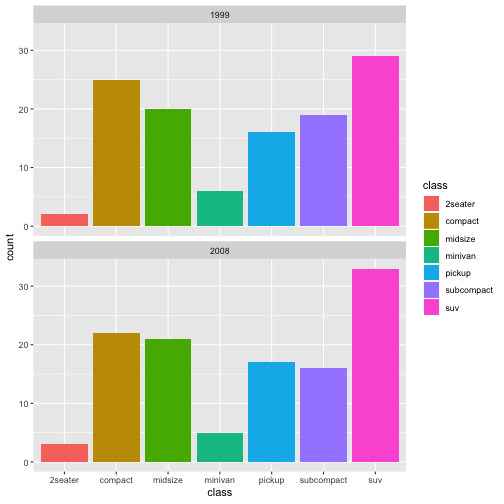
\includegraphics{bookdown-demo_files/figure-latex/unnamed-chunk-42-1.pdf}

\begin{Shaded}
\begin{Highlighting}[]
\KeywordTok{plot}\NormalTok{(mtcars}\OperatorTok{$}\NormalTok{wt, mtcars}\OperatorTok{$}\NormalTok{mpg,}
         \DataTypeTok{xlab=}\StringTok{"Miles Per Gallon"}\NormalTok{,}
         \DataTypeTok{ylab=}\StringTok{"Car Weight"}\NormalTok{)}
\KeywordTok{abline}\NormalTok{(}\KeywordTok{lm}\NormalTok{(mtcars}\OperatorTok{$}\NormalTok{mpg}\OperatorTok{~}\NormalTok{mtcars}\OperatorTok{$}\NormalTok{wt))}
\KeywordTok{title}\NormalTok{(}\StringTok{"Regression of MPG on Weight"}\NormalTok{)}
\end{Highlighting}
\end{Shaded}

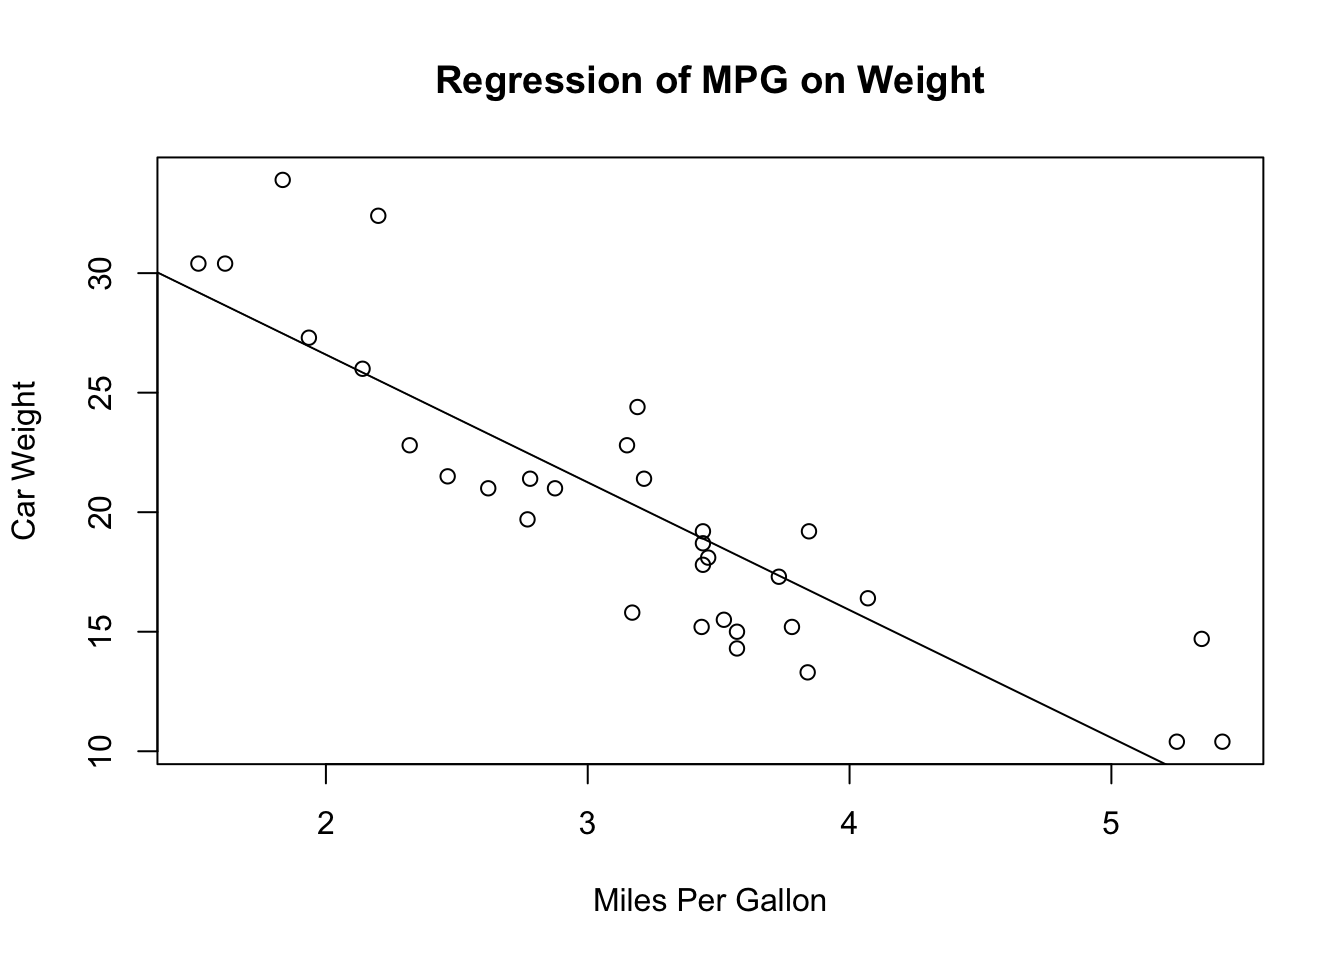
\includegraphics{bookdown-demo_files/figure-latex/unnamed-chunk-43-1.pdf}

第一条语句打开了一个图形窗口并生成了一幅散点图,横轴表
示车身重量,纵轴为每加仑汽油行驶的英里数。第二句向图形添加了一条最优拟合曲线。第三句
添加了标题。

\begin{Shaded}
\begin{Highlighting}[]
\KeywordTok{plot}\NormalTok{(mtcars}\OperatorTok{$}\NormalTok{wt, mtcars}\OperatorTok{$}\NormalTok{mpg,}
         \DataTypeTok{xlab=}\StringTok{"Miles Per Gallon"}\NormalTok{,}
         \DataTypeTok{ylab=}\StringTok{"Car Weight"}\NormalTok{,}
     \DataTypeTok{col=}\DecValTok{4}\NormalTok{)}
\KeywordTok{abline}\NormalTok{(}\KeywordTok{lm}\NormalTok{(mtcars}\OperatorTok{$}\NormalTok{mpg}\OperatorTok{~}\NormalTok{mtcars}\OperatorTok{$}\NormalTok{wt))}
\KeywordTok{title}\NormalTok{(}\StringTok{"Regression of MPG on Weight"}\NormalTok{)}
\end{Highlighting}
\end{Shaded}

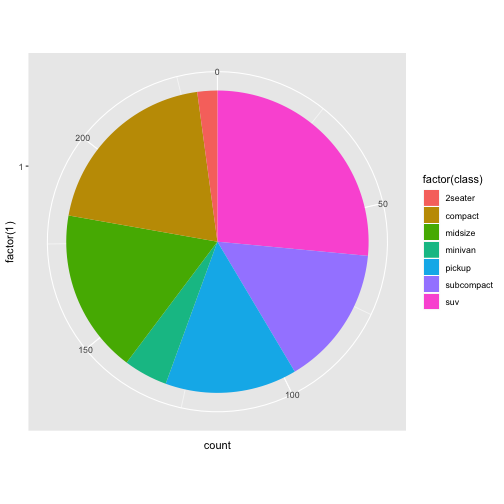
\includegraphics{bookdown-demo_files/figure-latex/unnamed-chunk-44-1.pdf}

\begin{Shaded}
\begin{Highlighting}[]
\KeywordTok{plot}\NormalTok{(mtcars}\OperatorTok{$}\NormalTok{wt, mtcars}\OperatorTok{$}\NormalTok{mpg,}
         \DataTypeTok{xlab=}\StringTok{"Miles Per Gallon"}\NormalTok{,}
         \DataTypeTok{ylab=}\StringTok{"Car Weight"}\NormalTok{,}
     \DataTypeTok{col=}\DecValTok{4}\NormalTok{,}
     \DataTypeTok{pch=}\DecValTok{16}\NormalTok{)}
\KeywordTok{abline}\NormalTok{(}\KeywordTok{lm}\NormalTok{(mtcars}\OperatorTok{$}\NormalTok{mpg}\OperatorTok{~}\NormalTok{mtcars}\OperatorTok{$}\NormalTok{wt))}
\KeywordTok{title}\NormalTok{(}\StringTok{"Regression of MPG on Weight"}\NormalTok{)}
\end{Highlighting}
\end{Shaded}

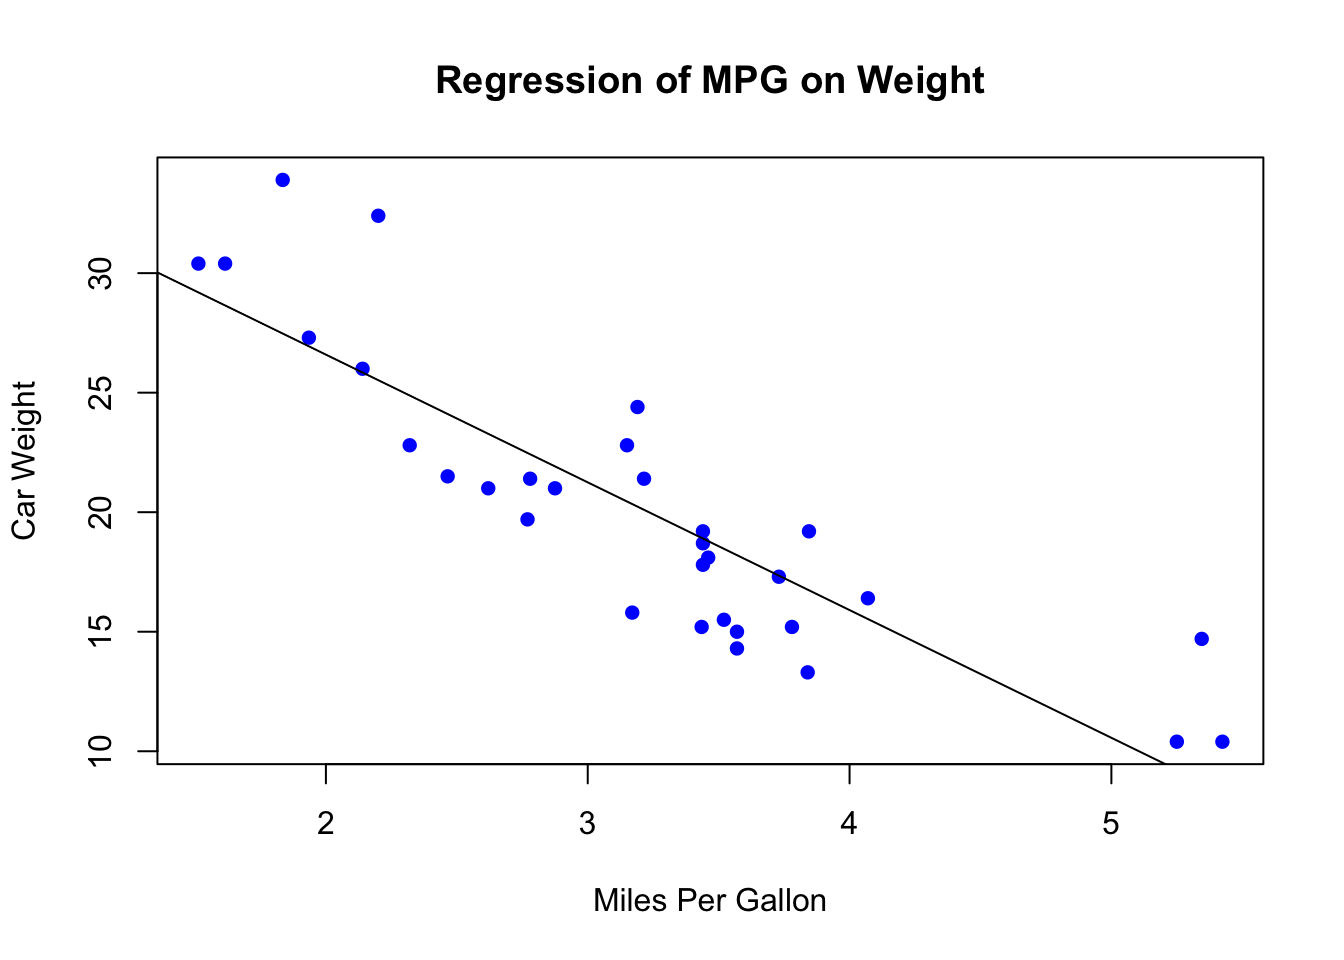
\includegraphics{bookdown-demo_files/figure-latex/unnamed-chunk-45-1.pdf}

总是用美元符号,是不是太麻烦?换一种方式:

\begin{Shaded}
\begin{Highlighting}[]
\KeywordTok{with}\NormalTok{(mtcars,\{}
\KeywordTok{plot}\NormalTok{(wt, mpg)}
\KeywordTok{abline}\NormalTok{(}\KeywordTok{lm}\NormalTok{(mpg}\OperatorTok{~}\NormalTok{wt))}
\KeywordTok{title}\NormalTok{(}\StringTok{"Regression of MPG on Weight"}\NormalTok{)}
\NormalTok{\}}
\NormalTok{)}
\end{Highlighting}
\end{Shaded}

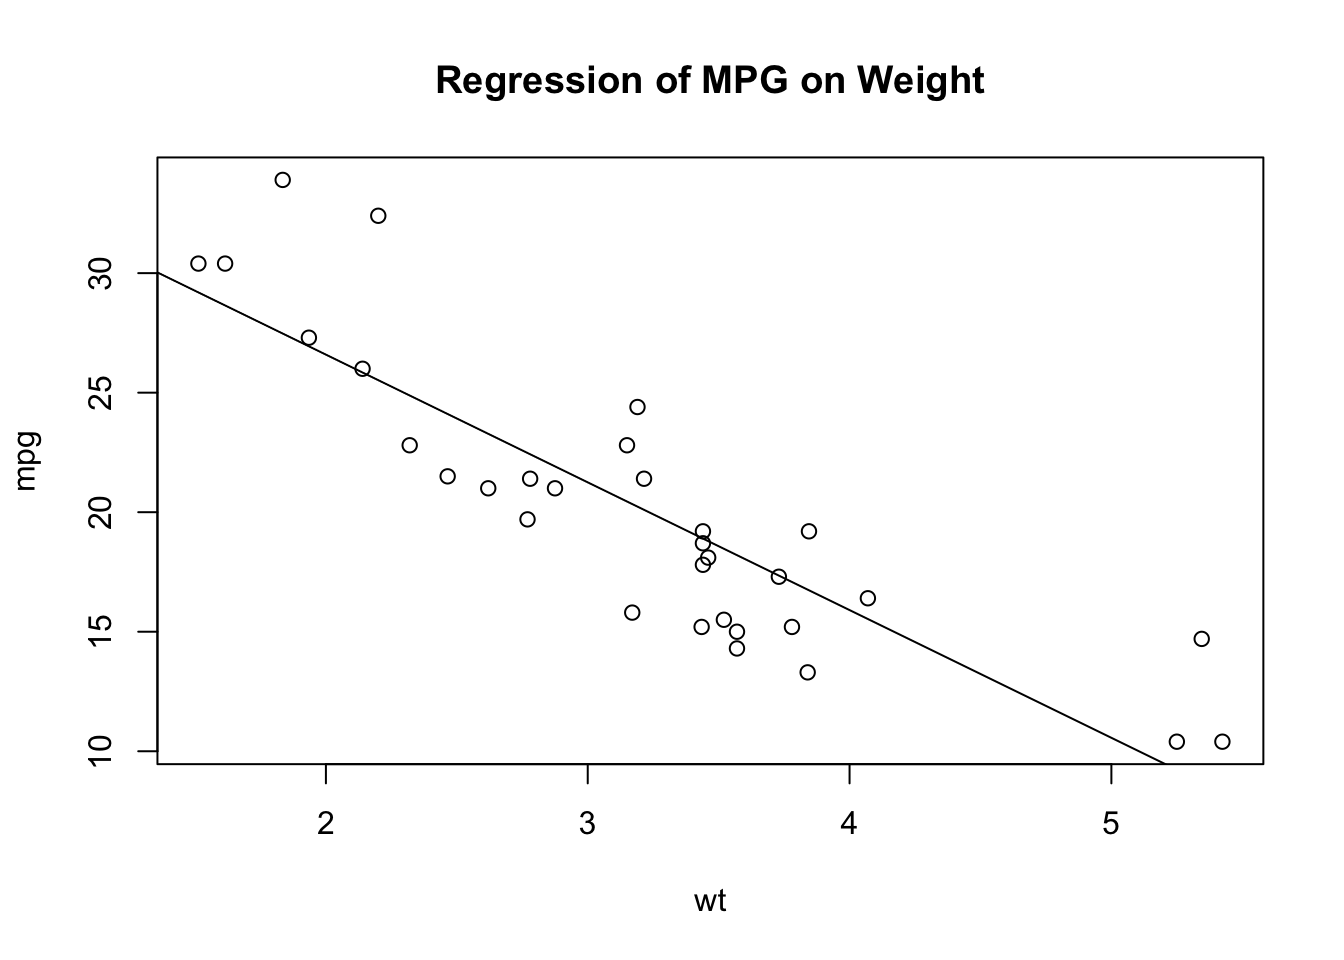
\includegraphics{bookdown-demo_files/figure-latex/unnamed-chunk-46-1.pdf}

全局参数设定,多图同列, 例如设置2列2行:

\begin{Shaded}
\begin{Highlighting}[]
\KeywordTok{par}\NormalTok{(}\DataTypeTok{mfrow=}\KeywordTok{c}\NormalTok{(}\DecValTok{3}\NormalTok{,}\DecValTok{1}\NormalTok{))}
\end{Highlighting}
\end{Shaded}

四个直方图:

\begin{Shaded}
\begin{Highlighting}[]
\KeywordTok{with}\NormalTok{(mtcars,\{}
  \KeywordTok{par}\NormalTok{(}\DataTypeTok{mfrow=}\KeywordTok{c}\NormalTok{(}\DecValTok{2}\NormalTok{,}\DecValTok{2}\NormalTok{))}
  \KeywordTok{hist}\NormalTok{(wt)}
  \KeywordTok{hist}\NormalTok{(mpg)}
  \KeywordTok{hist}\NormalTok{(disp)}
  \KeywordTok{hist}\NormalTok{(hp)}
\NormalTok{\})}
\end{Highlighting}
\end{Shaded}

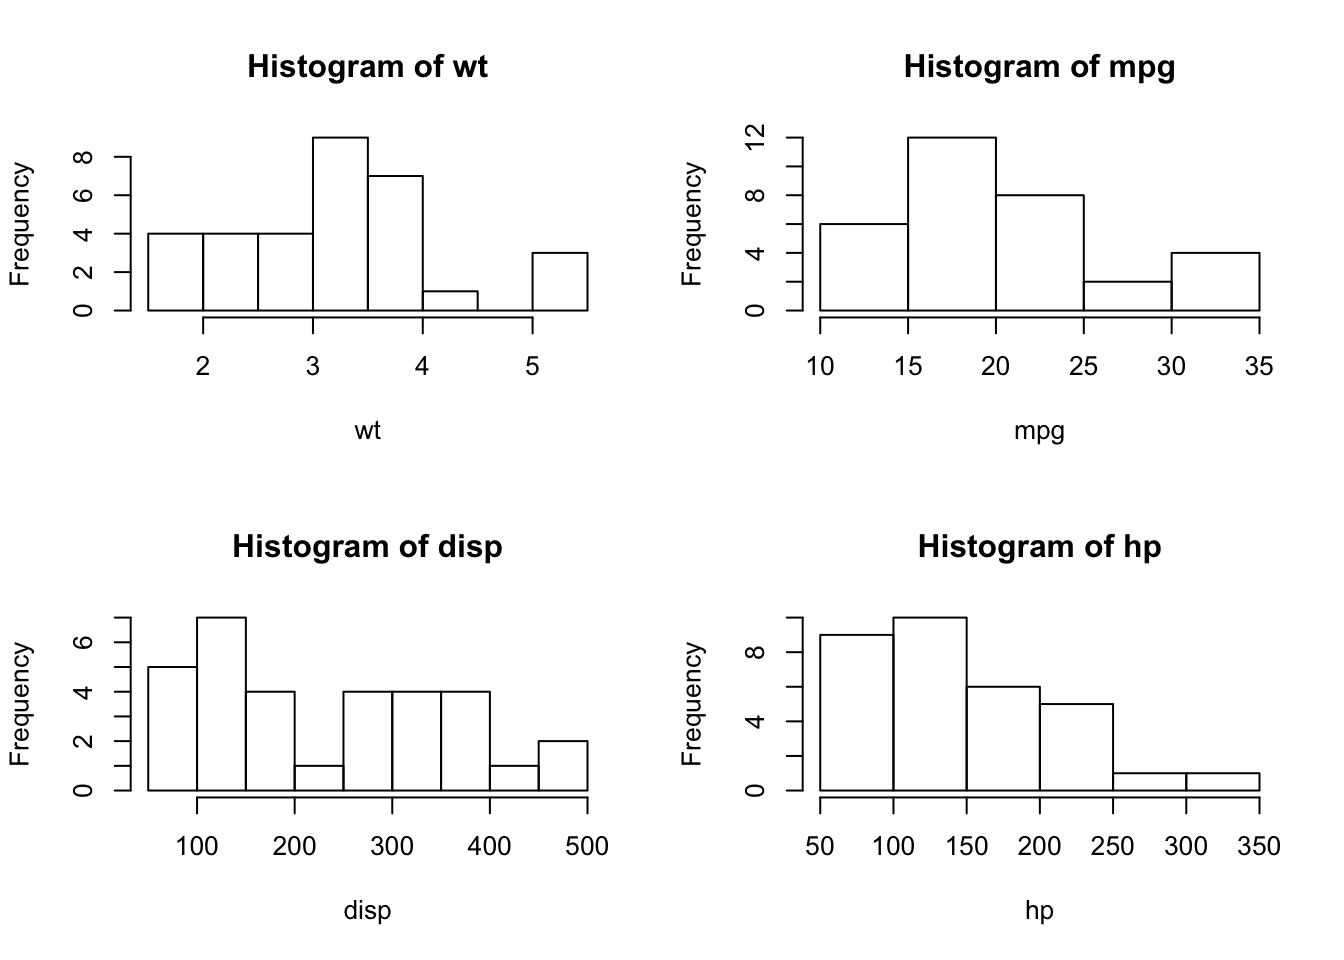
\includegraphics{bookdown-demo_files/figure-latex/unnamed-chunk-48-1.pdf}

箱图

\begin{Shaded}
\begin{Highlighting}[]
\KeywordTok{boxplot}\NormalTok{(mtcars}\OperatorTok{$}\NormalTok{mpg)}
\end{Highlighting}
\end{Shaded}

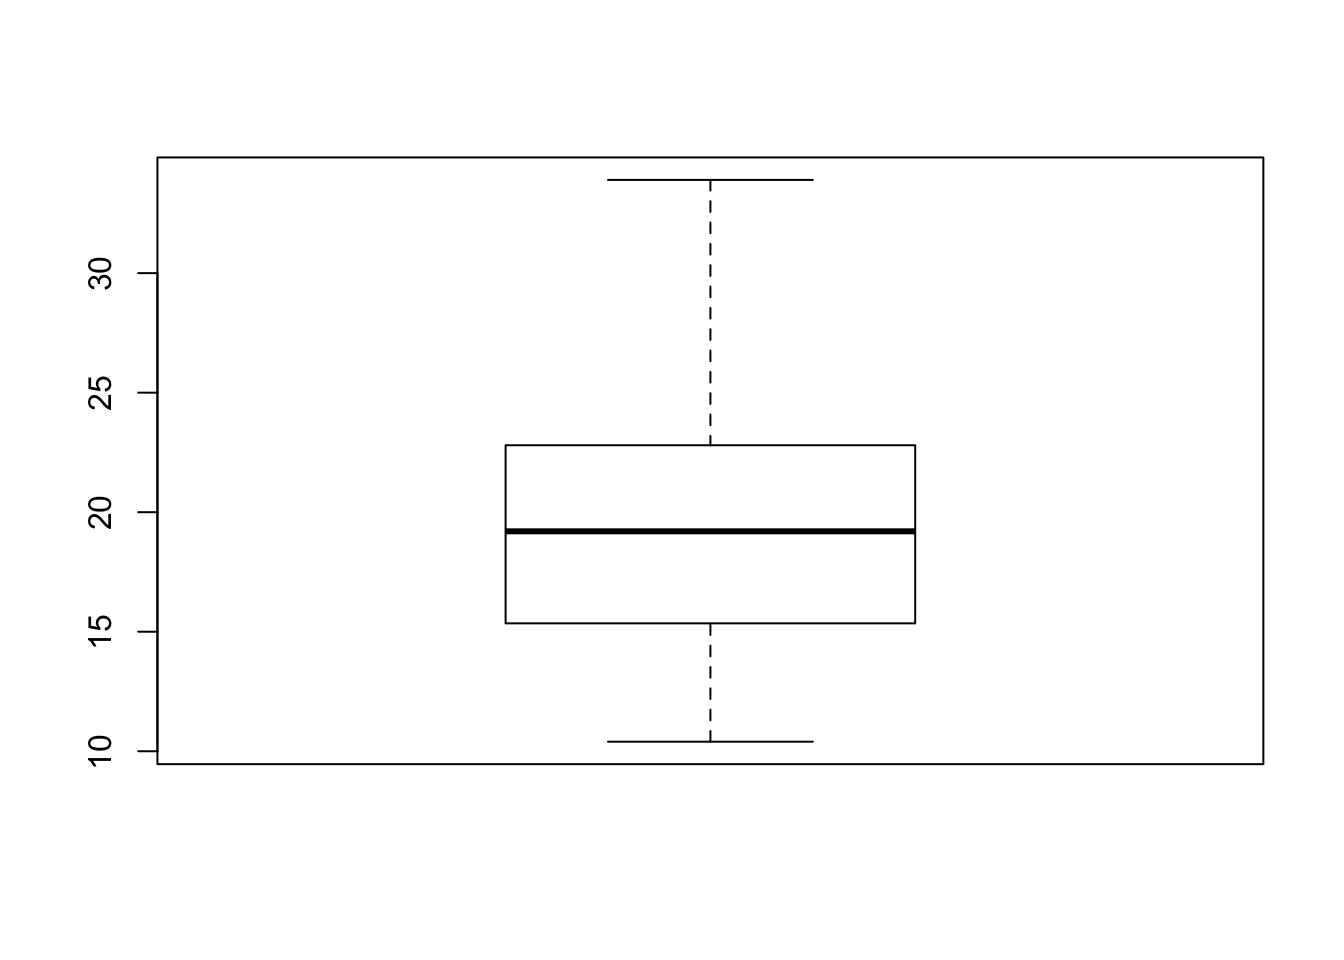
\includegraphics{bookdown-demo_files/figure-latex/unnamed-chunk-49-1.pdf}

可以通过代码或图形用户界面来保存图形。

要通过代码保存图形,将绘图语句夹在开启目标
图形设备的语句和关闭目标图形设备的语句之间即可。例如,以下代码会将图形保存到当前工作
目录中名为mygraph.pdf的PDF文件中(R in Action):

\begin{Shaded}
\begin{Highlighting}[]
\KeywordTok{pdf}\NormalTok{(}\StringTok{"mygraph.pdf"}\NormalTok{)}
      \KeywordTok{attach}\NormalTok{(mtcars)}
\end{Highlighting}
\end{Shaded}

\begin{verbatim}
## The following object is masked from package:ggplot2:
## 
##     mpg
\end{verbatim}

\begin{Shaded}
\begin{Highlighting}[]
      \KeywordTok{plot}\NormalTok{(wt, mpg)}
      \KeywordTok{abline}\NormalTok{(}\KeywordTok{lm}\NormalTok{(mpg}\OperatorTok{~}\NormalTok{wt))}
      \KeywordTok{title}\NormalTok{(}\StringTok{"Regression of MPG on Weight"}\NormalTok{)}
      \KeywordTok{detach}\NormalTok{(mtcars)}
\KeywordTok{dev.off}\NormalTok{()}
\end{Highlighting}
\end{Shaded}

\begin{verbatim}
## pdf 
##   2
\end{verbatim}

除了pdf(),还可以使用函数win.metafile()、png()、jpeg()、bmp()等将图形保存为其他格式。

通过图形用户界面保存图形,在RStudio的右下角,``Export''即可。

\chapter{数据管理}

\section{添加变量}

\section{缺失值处理}

\section{导入输入}

\section{脚本}

\hypertarget{rapply}{%
\chapter{掌握R语言中的apply函数族}\label{rapply}}

\url{http://blog.fens.me/r-apply/}

刚开始接触R语言时,会听到各种的R语言使用技巧,其中最重要的一条就是不要用循环,效率特别低,要用向量计算代替循环计算。

那么,这是为什么呢?原因在于R的循环操作for和while,都是基于R语言本身来实现的,而向量操作是基于底层的C语言函数实现的,从性能上来看,就会有比较明显的差距了。那么如何使用C的函数来实现向量计算呢,就是要用到apply的家族函数,包括apply,
sapply, tapply, mapply, lapply, rapply, vapply, eapply等。

\hypertarget{apply}{%
\section{apply的家族函数}\label{apply}}

apply函数族是R语言中数据处理的一组核心函数,通过使用apply函数,我们可以实现对数据的循环、分组、过滤、类型控制等操作。但是,由于在R语言中apply函数与其他语言循环体的处理思路是完全不一样的,所以apply函数族一直是使用者玩不转一类核心函数。

很多R语言新手,写了很多的for循环代码,也不愿意多花点时间把apply函数的使用方法了解清楚,最后把R代码写的跟C似得,我严重鄙视只会写for的R程序员。

apply函数本身就是解决数据循环处理的问题,为了面向不同的数据类型,不同的返回值,apply函数组成了一个函数族,包括了8个功能类似的函数。这其中有些函数很相似,有些也不是太一样的。

最常用的函数为apply和sapply,下面将分别介绍这8个函数的定义和使用方法。

\hypertarget{apply}{%
\section{apply函数}\label{apply}}

apply函数是最常用的代替for循环的函数。apply函数可以对矩阵、数据框、数组(二维、多维),按行或列进行循环计算,对子元素进行迭代,并把子元素以参数传递的形式给自定义的FUN函数中,并以返回计算结果。

函数定义:

\begin{Shaded}
\begin{Highlighting}[]
\KeywordTok{apply}\NormalTok{(X, MARGIN, FUN, ...)}
\end{Highlighting}
\end{Shaded}

参数列表:

\begin{itemize}
\tightlist
\item
  X:数组、矩阵、数据框
\item
  MARGIN: 按行计算或按按列计算,1表示按行,2表示按列
\item
  FUN: 自定义的调用函数
\item
  \ldots{}: 更多参数,可选
\end{itemize}

比如,对一个矩阵的每一行求和,下面就要用到apply做循环了。

\begin{Shaded}
\begin{Highlighting}[]
\NormalTok{x<-}\KeywordTok{matrix}\NormalTok{(}\DecValTok{1}\OperatorTok{:}\DecValTok{12}\NormalTok{,}\DataTypeTok{ncol=}\DecValTok{3}\NormalTok{)}
\KeywordTok{apply}\NormalTok{(x,}\DecValTok{1}\NormalTok{,sum)}
\end{Highlighting}
\end{Shaded}

\begin{verbatim}
## [1] 15 18 21 24
\end{verbatim}

下面计算一个稍微复杂点的例子,按行循环,让数据框的x1列加1,并计算出x1,x2列的均值。

生成data.frame

\begin{Shaded}
\begin{Highlighting}[]
\NormalTok{x <-}\StringTok{ }\KeywordTok{cbind}\NormalTok{(}\DataTypeTok{x1 =} \DecValTok{3}\NormalTok{, }\DataTypeTok{x2 =} \KeywordTok{c}\NormalTok{(}\DecValTok{4}\OperatorTok{:}\DecValTok{1}\NormalTok{, }\DecValTok{2}\OperatorTok{:}\DecValTok{5}\NormalTok{))}
\NormalTok{x}
\end{Highlighting}
\end{Shaded}

\begin{verbatim}
##      x1 x2
## [1,]  3  4
## [2,]  3  3
## [3,]  3  2
## [4,]  3  1
## [5,]  3  2
## [6,]  3  3
## [7,]  3  4
## [8,]  3  5
\end{verbatim}

\begin{Shaded}
\begin{Highlighting}[]
\CommentTok{# 自定义函数myFUN,第一个参数x为数据}
\CommentTok{# 第二、三个参数为自定义参数,可以通过apply的'...'进行传入。}
\NormalTok{myFUN<-}\StringTok{ }\ControlFlowTok{function}\NormalTok{(x, c1, c2) \{}
\KeywordTok{c}\NormalTok{(}\KeywordTok{sum}\NormalTok{(x[c1],}\DecValTok{1}\NormalTok{), }\KeywordTok{mean}\NormalTok{(x[c2])) }
\NormalTok{\}}

\CommentTok{# 把数据框按行做循环,每行分别传递给myFUN函数,设置c1,c2对应myFUN的第二、三个参数}
\KeywordTok{apply}\NormalTok{(x,}\DecValTok{1}\NormalTok{,myFUN,}\DataTypeTok{c1=}\StringTok{'x1'}\NormalTok{,}\DataTypeTok{c2=}\KeywordTok{c}\NormalTok{(}\StringTok{'x1'}\NormalTok{,}\StringTok{'x2'}\NormalTok{))}
\end{Highlighting}
\end{Shaded}

\begin{verbatim}
##      [,1] [,2] [,3] [,4] [,5] [,6] [,7] [,8]
## [1,]  4.0    4  4.0    4  4.0    4  4.0    4
## [2,]  3.5    3  2.5    2  2.5    3  3.5    4
\end{verbatim}

通过这个上面的自定义函数myFUN就实现了,一个常用的循环计算。

如果直接用for循环来实现,那么代码如下:

\begin{Shaded}
\begin{Highlighting}[]
\CommentTok{# 定义一个结果的数据框}
\NormalTok{df<-}\KeywordTok{data.frame}\NormalTok{()}

\CommentTok{# 定义for循环}
\ControlFlowTok{for}\NormalTok{(i }\ControlFlowTok{in} \DecValTok{1}\OperatorTok{:}\KeywordTok{nrow}\NormalTok{(x))\{}
\NormalTok{  row<-x[i,]                                         }\CommentTok{# 每行的值}
\NormalTok{  df<-}\KeywordTok{rbind}\NormalTok{(df,}\KeywordTok{rbind}\NormalTok{(}\KeywordTok{c}\NormalTok{(}\KeywordTok{sum}\NormalTok{(row[}\DecValTok{1}\NormalTok{],}\DecValTok{1}\NormalTok{), }\KeywordTok{mean}\NormalTok{(row))))    }\CommentTok{#计算,并赋值到结果数据框}
\NormalTok{  \}}

\CommentTok{# 打印结果数据框}
\NormalTok{df}
\end{Highlighting}
\end{Shaded}

通过for循环的方式,也可以很容易的实现上面计算过程,但是这里还有一些额外的操作需要自己处理,比如构建循环体、定义结果数据集、并合每次循环的结果到结果数据集。

对于上面的需求,还有第三种实现方法,那就是完成利用了R的特性,通过向量化计算来完成的。

\begin{Shaded}
\begin{Highlighting}[]
\KeywordTok{data.frame}\NormalTok{(}\DataTypeTok{x1=}\NormalTok{x[,}\DecValTok{1}\NormalTok{] }\DecValTok{1}\NormalTok{,}\DataTypeTok{x2=}\KeywordTok{rowMeans}\NormalTok{(x))}
\end{Highlighting}
\end{Shaded}

那么,一行就可以完成整个计算过程了。

接下来,我们需要再比较一下3种操作上面性能上的消耗。

\begin{Shaded}
\begin{Highlighting}[]
\CommentTok{# 清空环境变量}
 \KeywordTok{rm}\NormalTok{(}\DataTypeTok{list=}\KeywordTok{ls}\NormalTok{())}

\CommentTok{# 封装fun1}
\NormalTok{ fun1<-}\ControlFlowTok{function}\NormalTok{(x)\{}
\NormalTok{   myFUN<-}\StringTok{ }\ControlFlowTok{function}\NormalTok{(x, c1, c2) \{}
     \KeywordTok{c}\NormalTok{(}\KeywordTok{sum}\NormalTok{(x[c1],}\DecValTok{1}\NormalTok{), }\KeywordTok{mean}\NormalTok{(x[c2])) }
\NormalTok{   \}}
   \KeywordTok{apply}\NormalTok{(x,}\DecValTok{1}\NormalTok{,myFUN,}\DataTypeTok{c1=}\StringTok{'x1'}\NormalTok{,}\DataTypeTok{c2=}\KeywordTok{c}\NormalTok{(}\StringTok{'x1'}\NormalTok{,}\StringTok{'x2'}\NormalTok{))}
\NormalTok{ \}}

\CommentTok{# 封装fun2}
\NormalTok{ fun2<-}\ControlFlowTok{function}\NormalTok{(x)\{}
\NormalTok{   df<-}\KeywordTok{data.frame}\NormalTok{()}
   \ControlFlowTok{for}\NormalTok{(i }\ControlFlowTok{in} \DecValTok{1}\OperatorTok{:}\KeywordTok{nrow}\NormalTok{(x))\{}
\NormalTok{     row<-x[i,]}
\NormalTok{     df<-}\KeywordTok{rbind}\NormalTok{(df,}\KeywordTok{rbind}\NormalTok{(}\KeywordTok{c}\NormalTok{(}\KeywordTok{sum}\NormalTok{(row[}\DecValTok{1}\NormalTok{],}\DecValTok{1}\NormalTok{), }\KeywordTok{mean}\NormalTok{(row))))}
\NormalTok{   \}}
\NormalTok{ \}}

\CommentTok{# 封装fun3}
\NormalTok{ fun3<-}\ControlFlowTok{function}\NormalTok{(x)\{}
   \KeywordTok{data.frame}\NormalTok{(}\DataTypeTok{x1=}\NormalTok{x[,}\DecValTok{1}\NormalTok{]}\OperatorTok{+}\DecValTok{1}\NormalTok{,}\DataTypeTok{x2=}\KeywordTok{rowMeans}\NormalTok{(x))}
\NormalTok{ \}}

\CommentTok{# 生成数据集}
\NormalTok{x <-}\StringTok{ }\KeywordTok{cbind}\NormalTok{(}\DataTypeTok{x1=}\DecValTok{3}\NormalTok{, }\DataTypeTok{x2 =} \KeywordTok{c}\NormalTok{(}\DecValTok{400}\OperatorTok{:}\DecValTok{1}\NormalTok{, }\DecValTok{2}\OperatorTok{:}\DecValTok{500}\NormalTok{))}

\CommentTok{# 分别统计3种方法的CPU耗时。}
 \KeywordTok{system.time}\NormalTok{(}\KeywordTok{fun1}\NormalTok{(x))}
\end{Highlighting}
\end{Shaded}

\begin{verbatim}
##    user  system elapsed 
##   0.010   0.000   0.011
\end{verbatim}

\begin{Shaded}
\begin{Highlighting}[]
\KeywordTok{system.time}\NormalTok{(}\KeywordTok{fun2}\NormalTok{(x))}
\end{Highlighting}
\end{Shaded}

\begin{verbatim}
##    user  system elapsed 
##   0.163   0.008   0.171
\end{verbatim}

\begin{Shaded}
\begin{Highlighting}[]
\KeywordTok{system.time}\NormalTok{(}\KeywordTok{fun3}\NormalTok{(x))}
\end{Highlighting}
\end{Shaded}

\begin{verbatim}
##    user  system elapsed 
##       0       0       0
\end{verbatim}

从CPU的耗时来看,用for循环实现的计算是耗时最长的,apply实现的循环耗时很短,而直接使用R语言内置的向量计算的操作几乎不耗时。通过上面的测试,对同一个计算来说,优先考虑R语言内置的向量计算,必须要用到循环时则使用apply函数,应该尽量避免显示的使用for,while等操作方法。

\hypertarget{lapply}{%
\section{lapply函数}\label{lapply}}

lapply函数是一个最基础循环操作函数之一,用来对list、data.frame数据集进行循环,并返回和X长度同样的list结构作为结果集,通过lapply的开头的第一个字母'l'就可以判断返回结果集的类型。

函数定义:

\begin{Shaded}
\begin{Highlighting}[]
\KeywordTok{lapply}\NormalTok{(X, FUN, ...)}
\end{Highlighting}
\end{Shaded}

\hypertarget{dplyr-package}{%
\section{dplyr package}\label{dplyr-package}}

\hypertarget{r--base-graphics-in-r}{%
\chapter{R 基础作图快速入门 base graphics in
R}\label{r--base-graphics-in-r}}

导语:用数据说话的今天,随着数据量的不断增加,数据可视化成为将数字变成可用的信息的一个重要方式。

\begin{itemize}
\item
  Base graphics: 最容易上手, 同时也非常有用的绘图技巧,
  是这一节课的主要内容。
\item
  Grid graphics: 开发其它作图工具的强大工具
\item
  Lattice graphics: 基于 grid graphics的一般作图系统
\item
  ggplot2: 有语法,用写作的方式作图,非常炫酷,可视化必备
\end{itemize}

Base graphics:

\begin{Shaded}
\begin{Highlighting}[]
 \KeywordTok{library}\NormalTok{(MASS)}
\KeywordTok{plot}\NormalTok{(UScereal}\OperatorTok{$}\NormalTok{sugars, UScereal}\OperatorTok{$}\NormalTok{Calories)}
\KeywordTok{title}\NormalTok{(}\StringTok{"plot(UScereal$sugars, UScereal$calories)"}\NormalTok{)}
\end{Highlighting}
\end{Shaded}

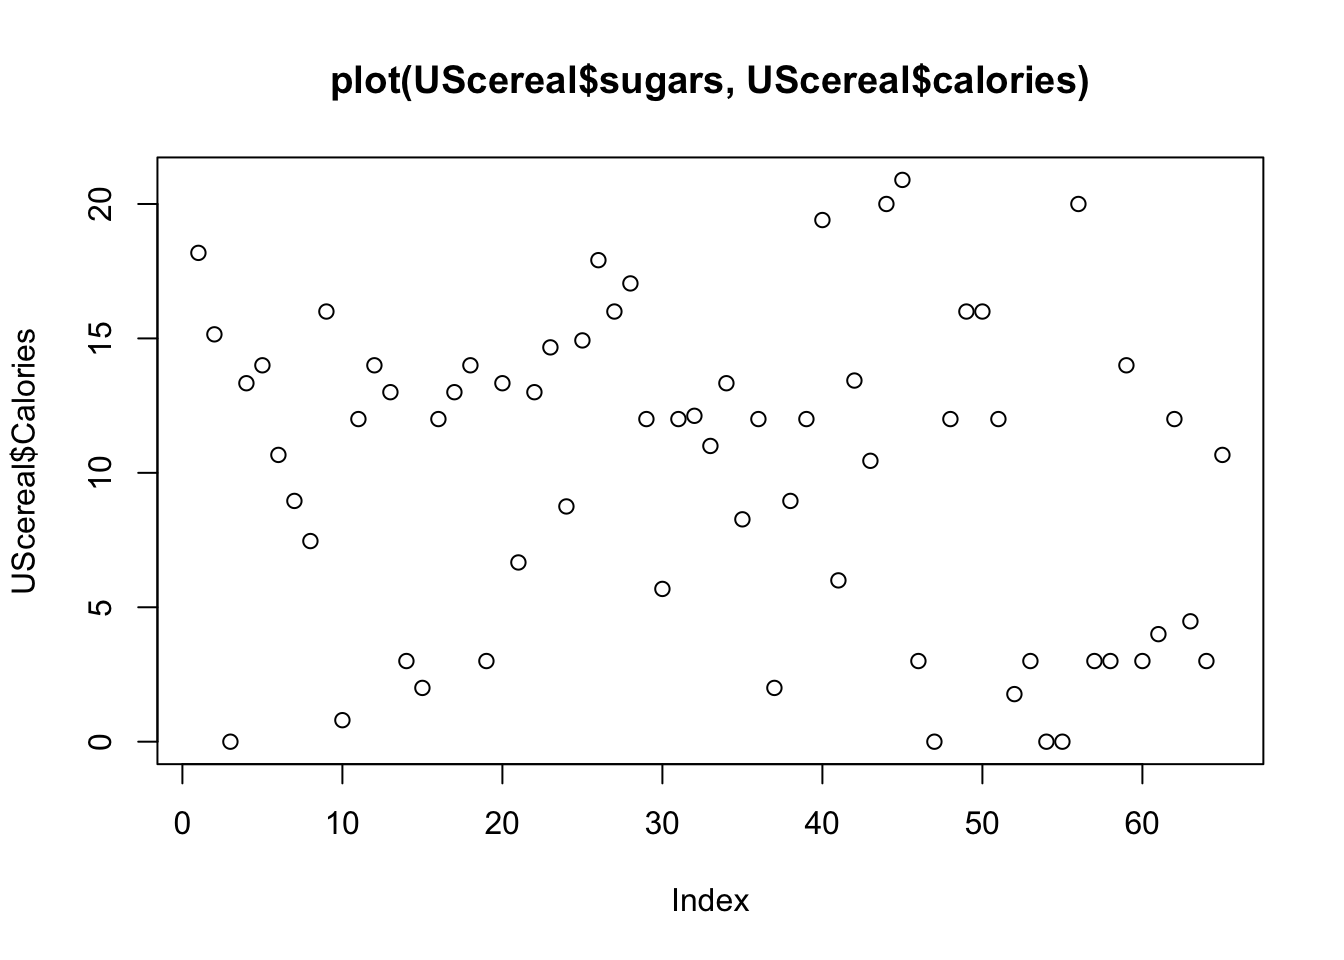
\includegraphics{bookdown-demo_files/figure-latex/unnamed-chunk-60-1.pdf}

Grid graphics,非人类的语言,不适用于一般的数据可视化:

\begin{Shaded}
\begin{Highlighting}[]
\CommentTok{# Get the data and load the grid package}
\KeywordTok{library}\NormalTok{(MASS)}
\NormalTok{x <-}\StringTok{ }\NormalTok{UScereal}\OperatorTok{$}\NormalTok{sugars}
\NormalTok{y <-}\StringTok{ }\NormalTok{UScereal}\OperatorTok{$}\NormalTok{calories}
\KeywordTok{library}\NormalTok{(grid)}
\CommentTok{# This is the grid code required to generate the plot}
\KeywordTok{pushViewport}\NormalTok{(}\KeywordTok{plotViewport}\NormalTok{())}
\KeywordTok{pushViewport}\NormalTok{(}\KeywordTok{dataViewport}\NormalTok{(x, y))}
\KeywordTok{grid.rect}\NormalTok{()}
\KeywordTok{grid.xaxis}\NormalTok{()}
\KeywordTok{grid.yaxis}\NormalTok{()}
\KeywordTok{grid.points}\NormalTok{(x, y)}
\KeywordTok{grid.text}\NormalTok{(}\StringTok{"UScereal$calories"}\NormalTok{, }\DataTypeTok{x =} \KeywordTok{unit}\NormalTok{(}\OperatorTok{-}\DecValTok{3}\NormalTok{, }\StringTok{"lines"}\NormalTok{), }\DataTypeTok{rot =} \DecValTok{90}\NormalTok{)}
\KeywordTok{grid.text}\NormalTok{(}\StringTok{"UScereal$sugars"}\NormalTok{, }\DataTypeTok{y =} \KeywordTok{unit}\NormalTok{(}\OperatorTok{-}\DecValTok{3}\NormalTok{, }\StringTok{"lines"}\NormalTok{), }\DataTypeTok{rot =} \DecValTok{0}\NormalTok{)}
\KeywordTok{popViewport}\NormalTok{(}\DecValTok{2}\NormalTok{)}
\end{Highlighting}
\end{Shaded}

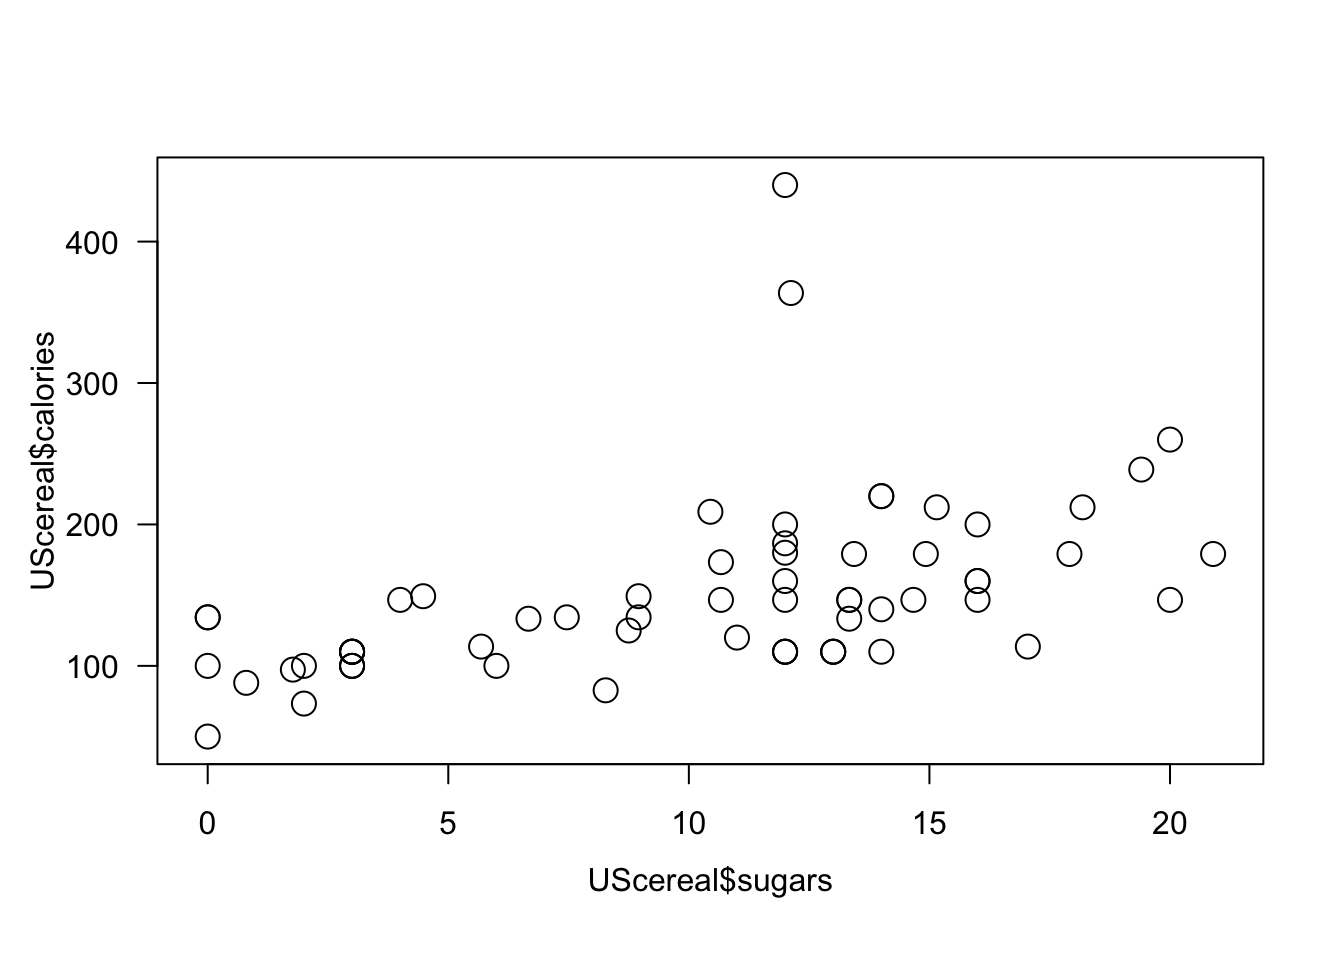
\includegraphics{bookdown-demo_files/figure-latex/unnamed-chunk-61-1.pdf}

Lattice graphics:

\begin{Shaded}
\begin{Highlighting}[]
\KeywordTok{library}\NormalTok{(MASS)}
\KeywordTok{library}\NormalTok{(lattice)}
\KeywordTok{xyplot}\NormalTok{(MPG.city }\OperatorTok{~}\StringTok{ }\NormalTok{Horsepower }\OperatorTok{|}\StringTok{ }\NormalTok{Cylinders, }\DataTypeTok{data =}\NormalTok{ Cars93)}
\end{Highlighting}
\end{Shaded}

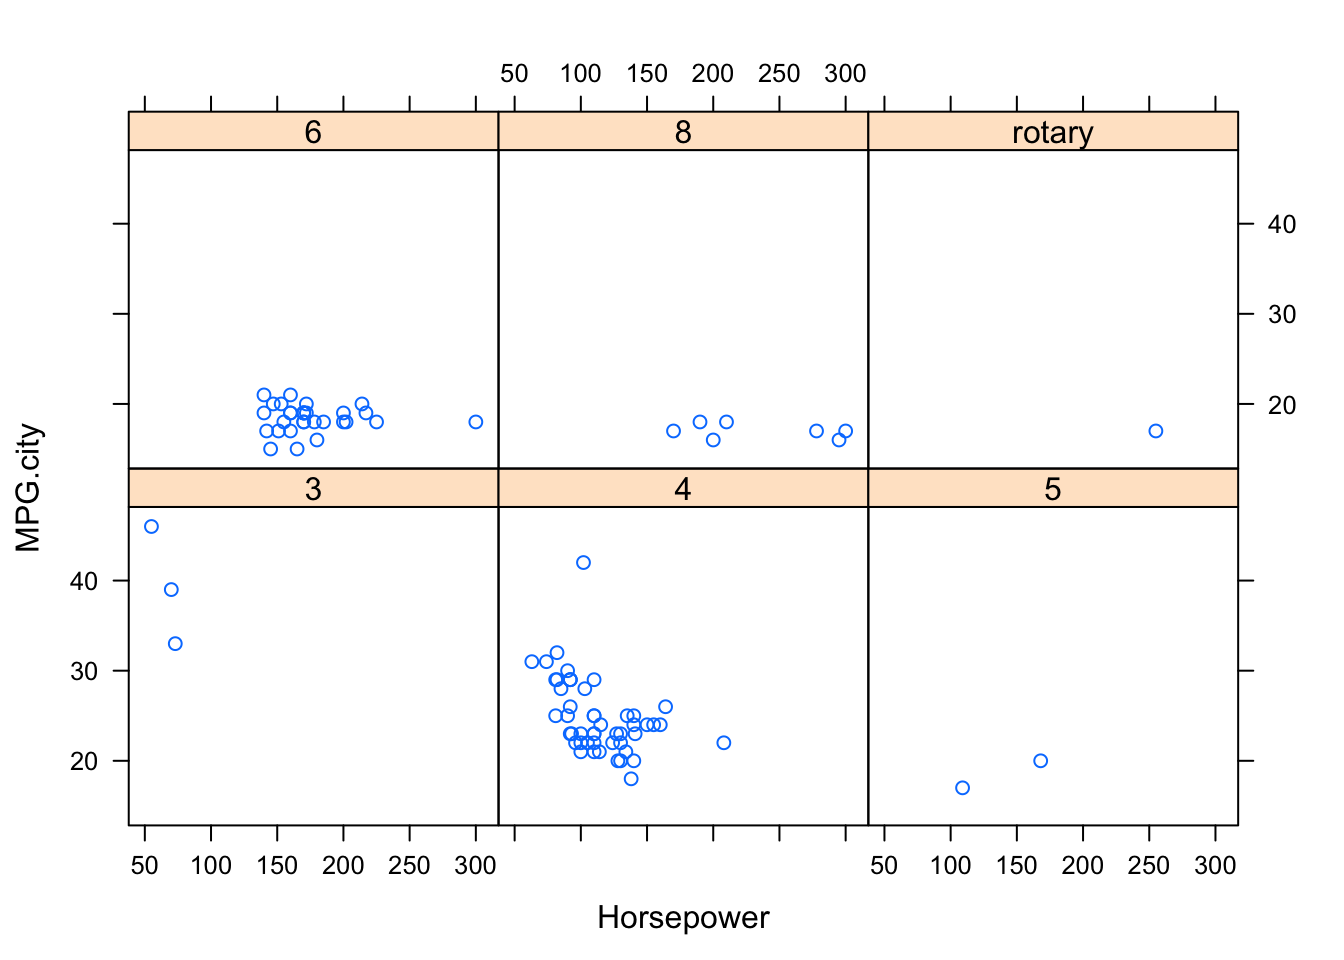
\includegraphics{bookdown-demo_files/figure-latex/unnamed-chunk-62-1.pdf}

ggplot2:

\begin{Shaded}
\begin{Highlighting}[]
\KeywordTok{library}\NormalTok{(MASS)}
\KeywordTok{library}\NormalTok{(ggplot2)}
\NormalTok{title <-}
\StringTok{ "ggplot2 plot of }\CharTok{\textbackslash{}n}\StringTok{ UScereal$calories vs. }\CharTok{\textbackslash{}n}\StringTok{ UScereal$sugars"}
\NormalTok{basePlot <-}\StringTok{ }\KeywordTok{ggplot}\NormalTok{(UScereal, }\KeywordTok{aes}\NormalTok{(}\DataTypeTok{x =}\NormalTok{ sugars, }\DataTypeTok{y =}\NormalTok{ calories))}
\NormalTok{basePlot }\OperatorTok{+}
\StringTok{ }\KeywordTok{geom_point}\NormalTok{(}\DataTypeTok{shape =} \KeywordTok{as.character}\NormalTok{(UScereal}\OperatorTok{$}\NormalTok{shelf), }\DataTypeTok{size =} \DecValTok{3}\NormalTok{) }\OperatorTok{+}
\StringTok{ }\KeywordTok{annotate}\NormalTok{(}\StringTok{"text"}\NormalTok{, }\DataTypeTok{label =}\NormalTok{ title, }\DataTypeTok{x =} \DecValTok{3}\NormalTok{, }\DataTypeTok{y =} \DecValTok{400}\NormalTok{,}
 \DataTypeTok{colour =} \StringTok{"red"}\NormalTok{)}
\end{Highlighting}
\end{Shaded}

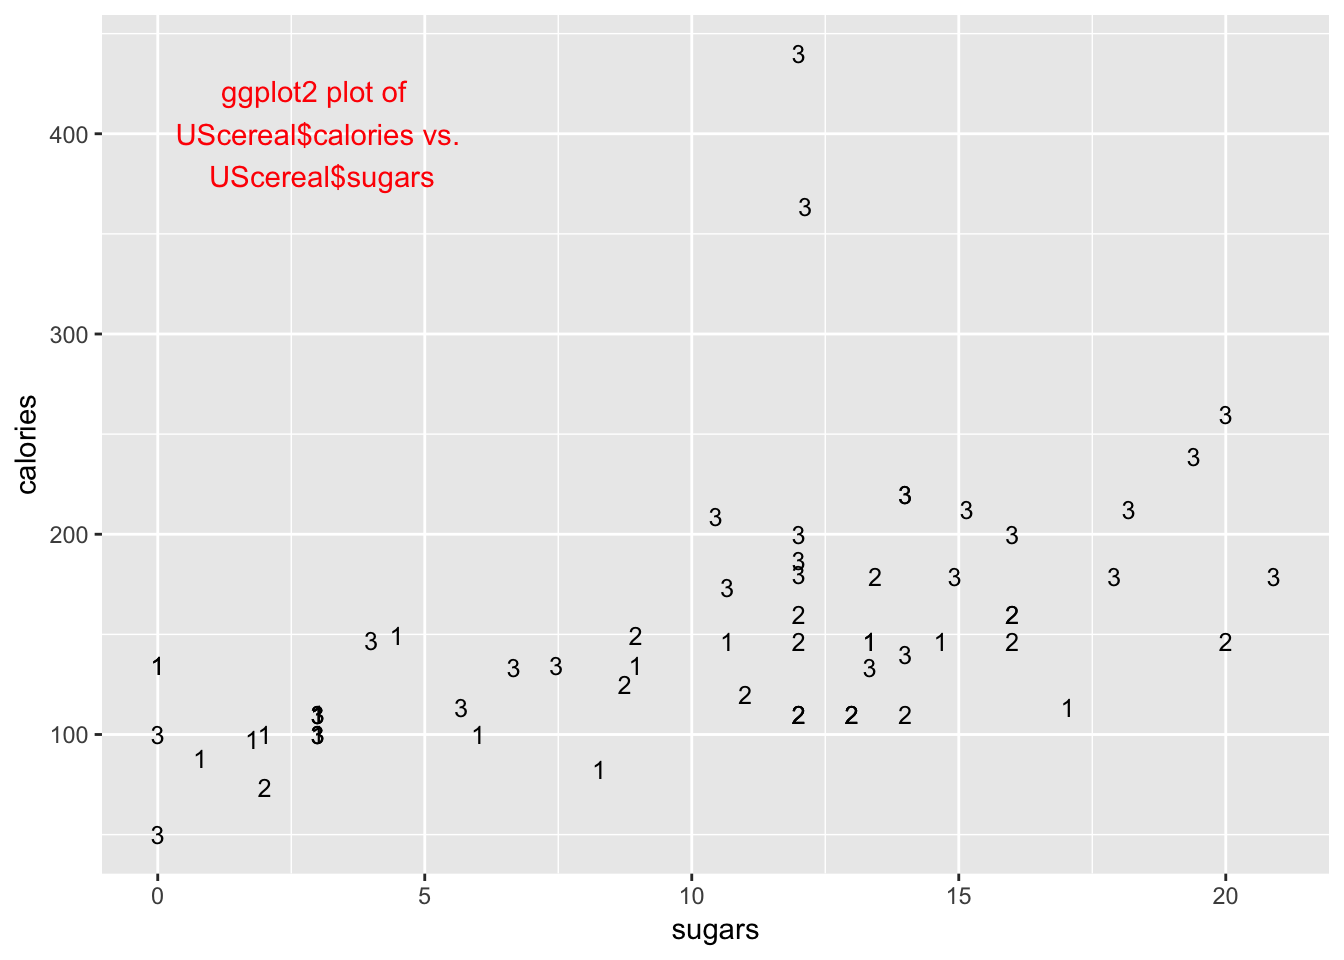
\includegraphics{bookdown-demo_files/figure-latex/unnamed-chunk-63-1.pdf}

\begin{itemize}
\tightlist
\item
  探索性数据可视化:
  帮助你看一看数据里都有什么,注意尽量多地保留细节,便于进一步分析
\end{itemize}

探索小鸡的成长之路:ChickWeight数据集

\begin{Shaded}
\begin{Highlighting}[]
\KeywordTok{plot}\NormalTok{(ChickWeight)}
\end{Highlighting}
\end{Shaded}

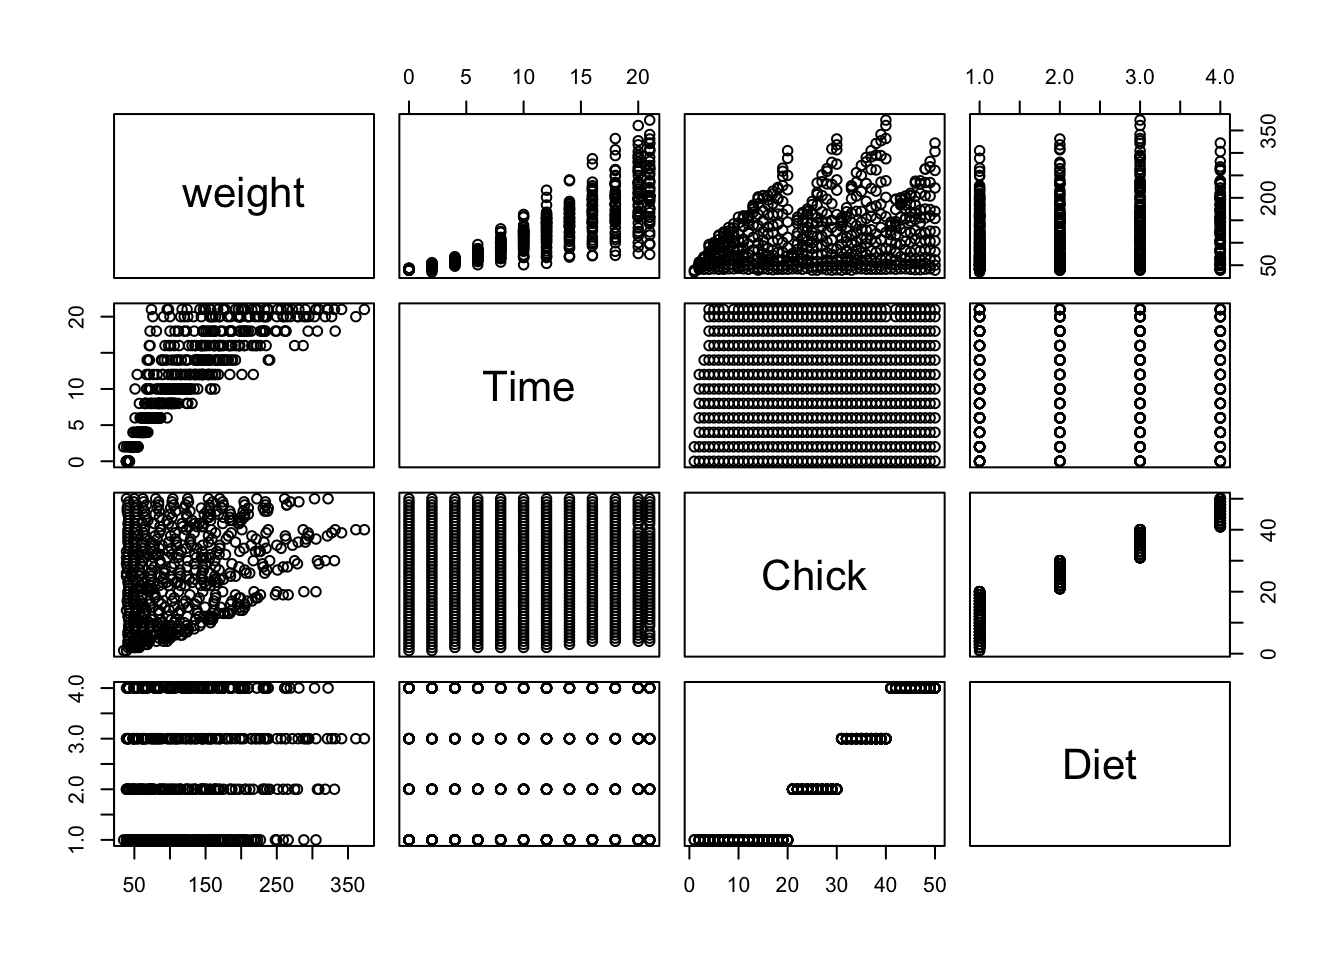
\includegraphics{bookdown-demo_files/figure-latex/unnamed-chunk-64-1.pdf}

\begin{itemize}
\tightlist
\item
  解释性数据可视化:让别人明白数据,便于交流信息,呈现你的数据发现
\end{itemize}

请在下面的练习开始前,下载并安装下面这些包:

\begin{Shaded}
\begin{Highlighting}[]
\KeywordTok{install.packages}\NormalTok{(}\StringTok{"insuranceData"}\NormalTok{)}
\KeywordTok{install.packages}\NormalTok{(}\StringTok{"MASS"}\NormalTok{)}
\KeywordTok{install.packages}\NormalTok{(}\StringTok{"robustbase"}\NormalTok{)}
\KeywordTok{install.packages}\NormalTok{(}\StringTok{"car"}\NormalTok{)}
\KeywordTok{install.packages}\NormalTok{(}\StringTok{"aplpack"}\NormalTok{)}
\KeywordTok{install.packages}\NormalTok{(}\StringTok{"corrplot"}\NormalTok{)}
\KeywordTok{install.packages}\NormalTok{(}\StringTok{"rpart"}\NormalTok{)}
\end{Highlighting}
\end{Shaded}

\begin{Shaded}
\begin{Highlighting}[]
\CommentTok{# Load MASS package}
\KeywordTok{library}\NormalTok{(dplyr)}
\KeywordTok{library}\NormalTok{(MASS)}
\KeywordTok{library}\NormalTok{(robustbase)}
\KeywordTok{library}\NormalTok{(insuranceData)}
\KeywordTok{library}\NormalTok{(car)}
\end{Highlighting}
\end{Shaded}

我们用一个简单的冬季取暖数据来建构一个简单的分析图: Temp:
一周的室外气温 Gas: 该周的天然气用量 Insul:
有两个值的分类变量,分别代表房子升级改造前后

简单绘图看一下:

\begin{Shaded}
\begin{Highlighting}[]
\CommentTok{# Plot whiteside data}
\KeywordTok{plot}\NormalTok{(whiteside)}
\end{Highlighting}
\end{Shaded}

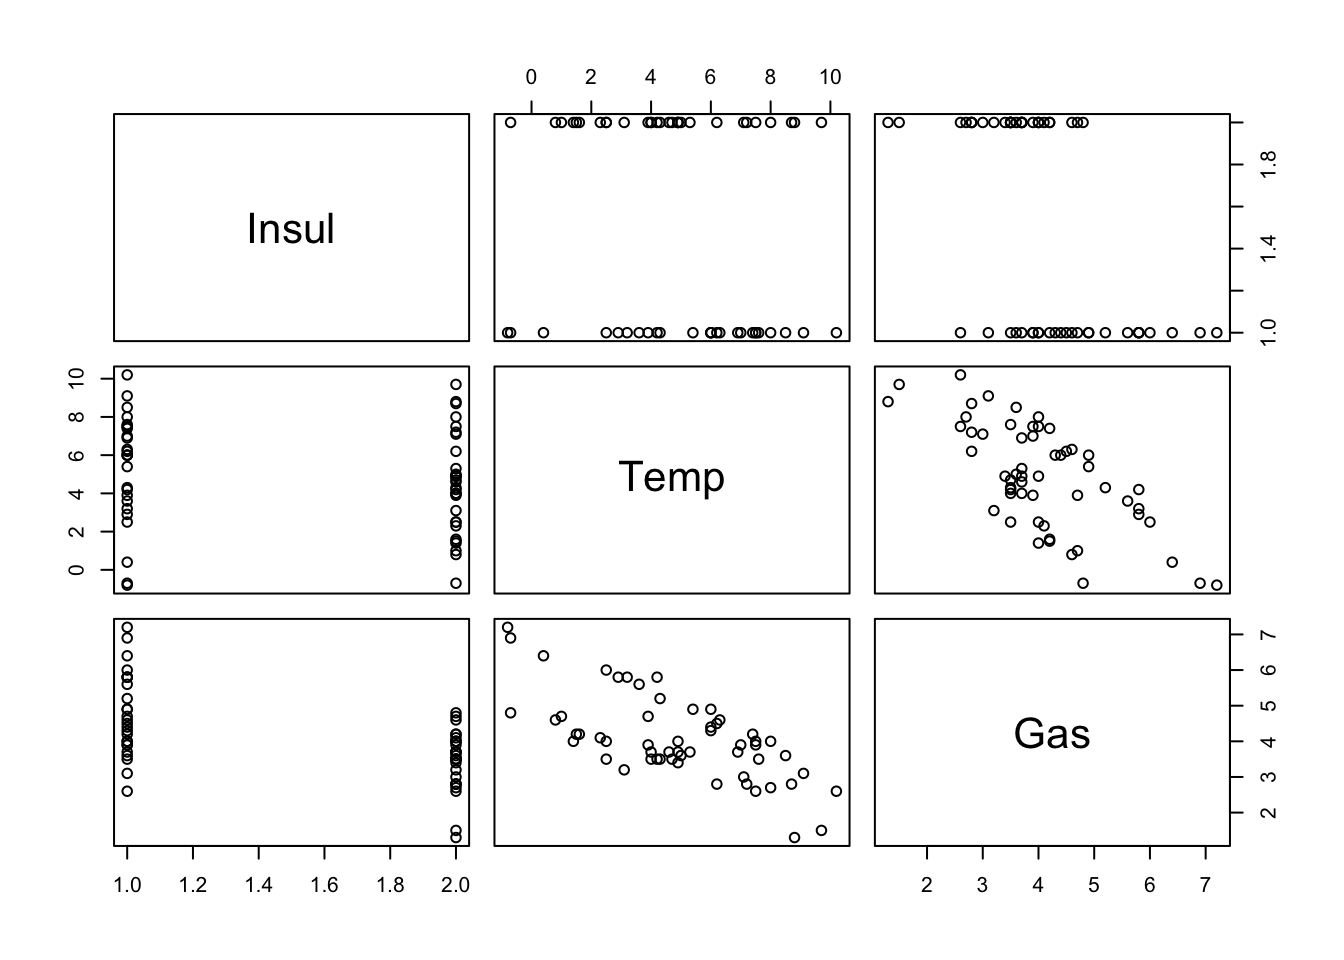
\includegraphics{bookdown-demo_files/figure-latex/unnamed-chunk-67-1.pdf}

简单的探索性散点图:
不要完全依赖默认设置,适当修改,让图更有意义容易理解
做一个气温与天然气用量的散点图,加上轴标签:

\begin{Shaded}
\begin{Highlighting}[]
\KeywordTok{plot}\NormalTok{(whiteside}\OperatorTok{$}\NormalTok{Temp,whiteside}\OperatorTok{$}\NormalTok{Gas,}
     \DataTypeTok{xlab=}\StringTok{"Outside temperature"}\NormalTok{,}
     \DataTypeTok{ylab=} \StringTok{"Heating gas consumption"}\NormalTok{)}
\end{Highlighting}
\end{Shaded}

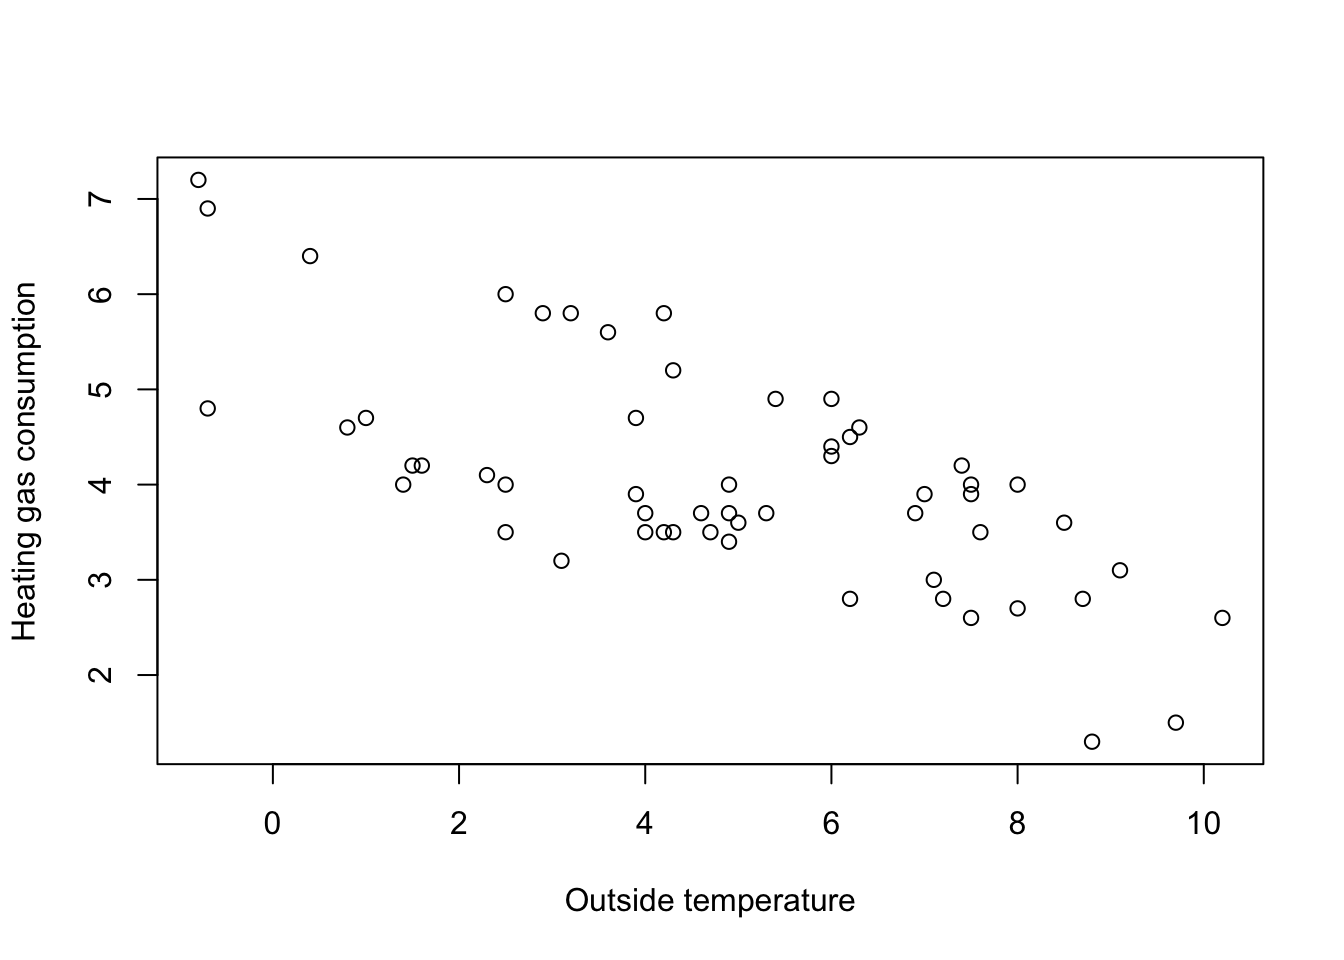
\includegraphics{bookdown-demo_files/figure-latex/unnamed-chunk-68-1.pdf}

\texttt{plot()}是一个一般性的函数,会根据数据类型的不同而作出不同的图,例如下面,我们把它用在\texttt{whiteside\$Insul}上,得到一个完全不一样的图

\begin{Shaded}
\begin{Highlighting}[]
\KeywordTok{plot}\NormalTok{(whiteside}\OperatorTok{$}\NormalTok{Insul)}
\end{Highlighting}
\end{Shaded}

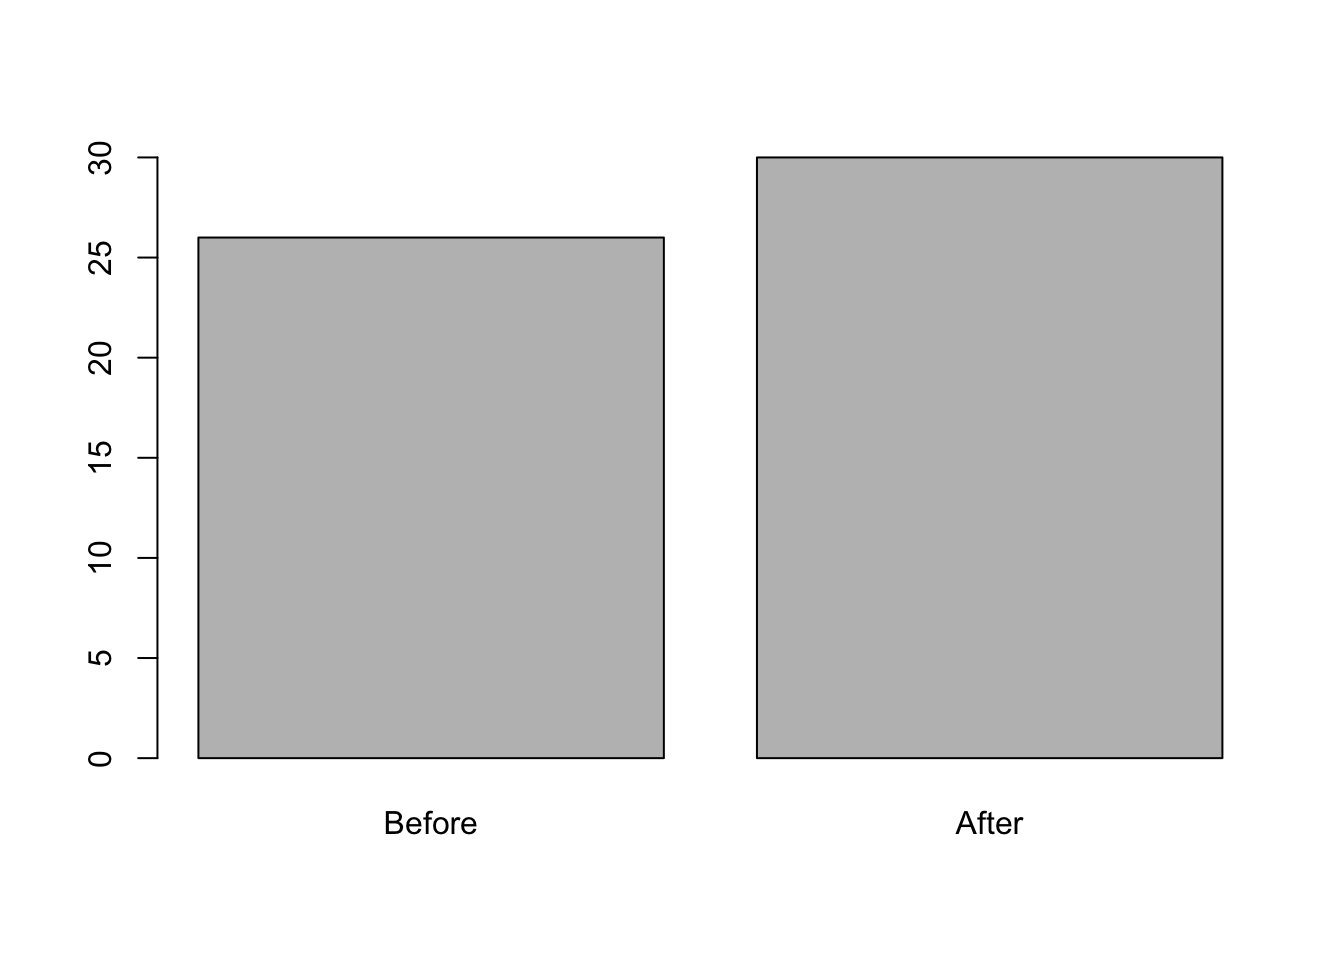
\includegraphics{bookdown-demo_files/figure-latex/unnamed-chunk-69-1.pdf}

使用形状,颜色和参考线来增加细节,我们用Cars93这个数据集来做一个高级一点的图来展示三个变量间的关系:

Price: 某款车的平均售价 Max.Price: 该款车的最高售价 Min.Price:
该款车的最低售价

使用 \texttt{glimpse()} 来看看这个Cars93 都有什么变量

\begin{Shaded}
\begin{Highlighting}[]
\KeywordTok{glimpse}\NormalTok{(Cars93)}
\end{Highlighting}
\end{Shaded}

\begin{verbatim}
## Observations: 93
## Variables: 27
## $ Manufacturer       <fct> Acura, Acura, Audi, Audi, BMW, Buick, Buick...
## $ Model              <fct> Integra, Legend, 90, 100, 535i, Century, Le...
## $ Type               <fct> Small, Midsize, Compact, Midsize, Midsize, ...
## $ Min.Price          <dbl> 12.9, 29.2, 25.9, 30.8, 23.7, 14.2, 19.9, 2...
## $ Price              <dbl> 15.9, 33.9, 29.1, 37.7, 30.0, 15.7, 20.8, 2...
## $ Max.Price          <dbl> 18.8, 38.7, 32.3, 44.6, 36.2, 17.3, 21.7, 2...
## $ MPG.city           <int> 25, 18, 20, 19, 22, 22, 19, 16, 19, 16, 16,...
## $ MPG.highway        <int> 31, 25, 26, 26, 30, 31, 28, 25, 27, 25, 25,...
## $ AirBags            <fct> None, Driver & Passenger, Driver only, Driv...
## $ DriveTrain         <fct> Front, Front, Front, Front, Rear, Front, Fr...
## $ Cylinders          <fct> 4, 6, 6, 6, 4, 4, 6, 6, 6, 8, 8, 4, 4, 6, 4...
## $ EngineSize         <dbl> 1.8, 3.2, 2.8, 2.8, 3.5, 2.2, 3.8, 5.7, 3.8...
## $ Horsepower         <int> 140, 200, 172, 172, 208, 110, 170, 180, 170...
## $ RPM                <int> 6300, 5500, 5500, 5500, 5700, 5200, 4800, 4...
## $ Rev.per.mile       <int> 2890, 2335, 2280, 2535, 2545, 2565, 1570, 1...
## $ Man.trans.avail    <fct> Yes, Yes, Yes, Yes, Yes, No, No, No, No, No...
## $ Fuel.tank.capacity <dbl> 13.2, 18.0, 16.9, 21.1, 21.1, 16.4, 18.0, 2...
## $ Passengers         <int> 5, 5, 5, 6, 4, 6, 6, 6, 5, 6, 5, 5, 5, 4, 6...
## $ Length             <int> 177, 195, 180, 193, 186, 189, 200, 216, 198...
## $ Wheelbase          <int> 102, 115, 102, 106, 109, 105, 111, 116, 108...
## $ Width              <int> 68, 71, 67, 70, 69, 69, 74, 78, 73, 73, 74,...
## $ Turn.circle        <int> 37, 38, 37, 37, 39, 41, 42, 45, 41, 43, 44,...
## $ Rear.seat.room     <dbl> 26.5, 30.0, 28.0, 31.0, 27.0, 28.0, 30.5, 3...
## $ Luggage.room       <int> 11, 15, 14, 17, 13, 16, 17, 21, 14, 18, 14,...
## $ Weight             <int> 2705, 3560, 3375, 3405, 3640, 2880, 3470, 4...
## $ Origin             <fct> non-USA, non-USA, non-USA, non-USA, non-USA...
## $ Make               <fct> Acura Integra, Acura Legend, Audi 90, Audi ...
\end{verbatim}

最高价vs.平均价,红色三角

\begin{Shaded}
\begin{Highlighting}[]
\KeywordTok{plot}\NormalTok{(Cars93}\OperatorTok{$}\NormalTok{Max.Price, Cars93}\OperatorTok{$}\NormalTok{Price,}\DataTypeTok{col=}\StringTok{"red"}\NormalTok{,}\DataTypeTok{pch=}\DecValTok{17}\NormalTok{)}
\end{Highlighting}
\end{Shaded}

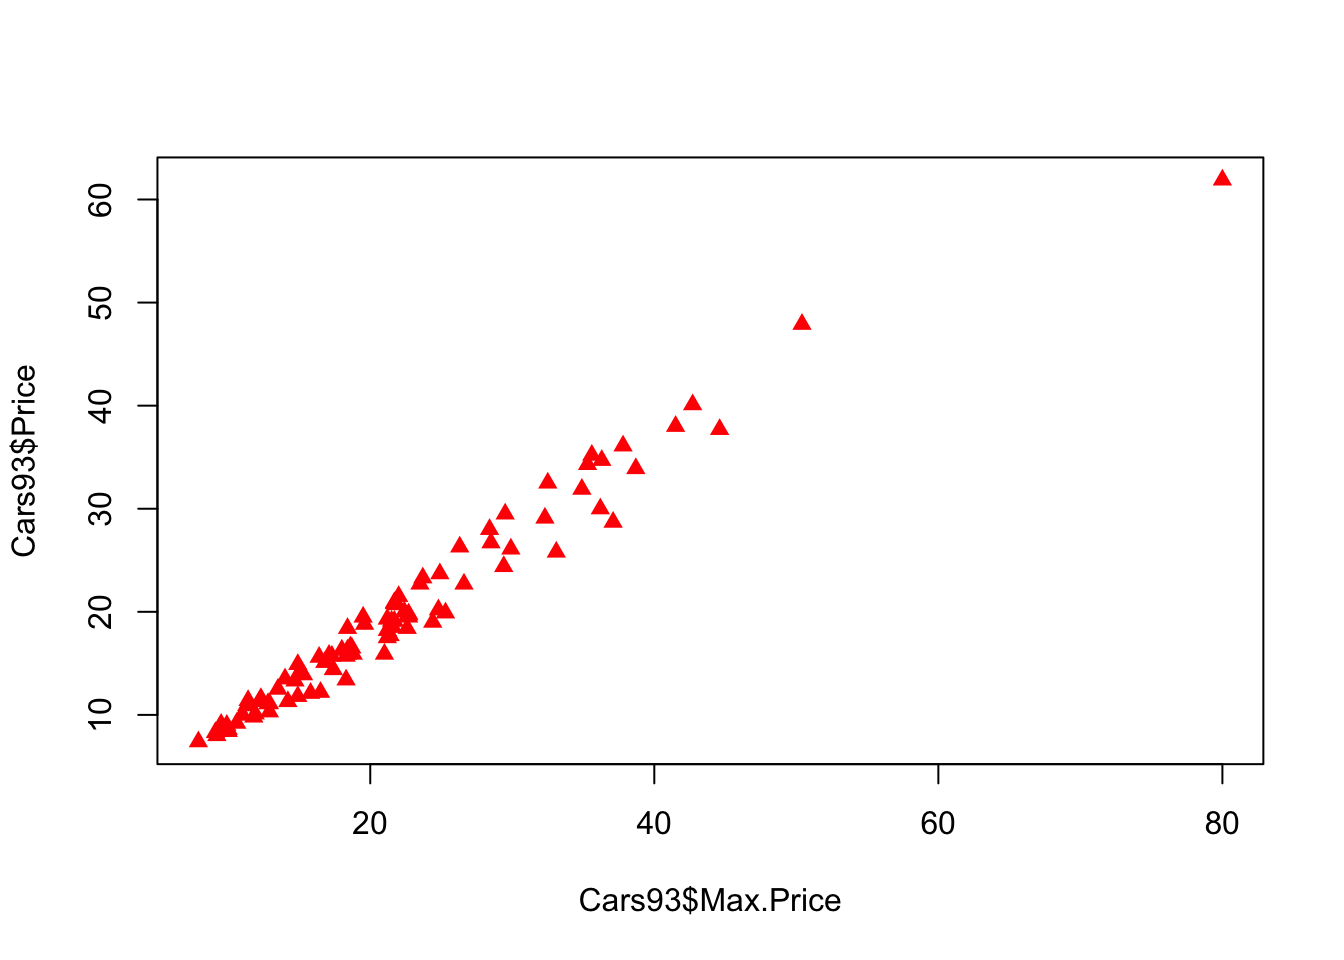
\includegraphics{bookdown-demo_files/figure-latex/unnamed-chunk-71-1.pdf}

添加最高价vs. 平均价,蓝色,圆点

\begin{Shaded}
\begin{Highlighting}[]
\KeywordTok{plot}\NormalTok{(Cars93}\OperatorTok{$}\NormalTok{Max.Price, Cars93}\OperatorTok{$}\NormalTok{Price,}\DataTypeTok{col=}\StringTok{"red"}\NormalTok{,}\DataTypeTok{pch=}\DecValTok{17}\NormalTok{)}
\KeywordTok{points}\NormalTok{(Cars93}\OperatorTok{$}\NormalTok{Min.Price,Cars93}\OperatorTok{$}\NormalTok{Price,}\DataTypeTok{col=}\StringTok{"blue"}\NormalTok{,}\DataTypeTok{pch=}\DecValTok{16}\NormalTok{)}
\end{Highlighting}
\end{Shaded}

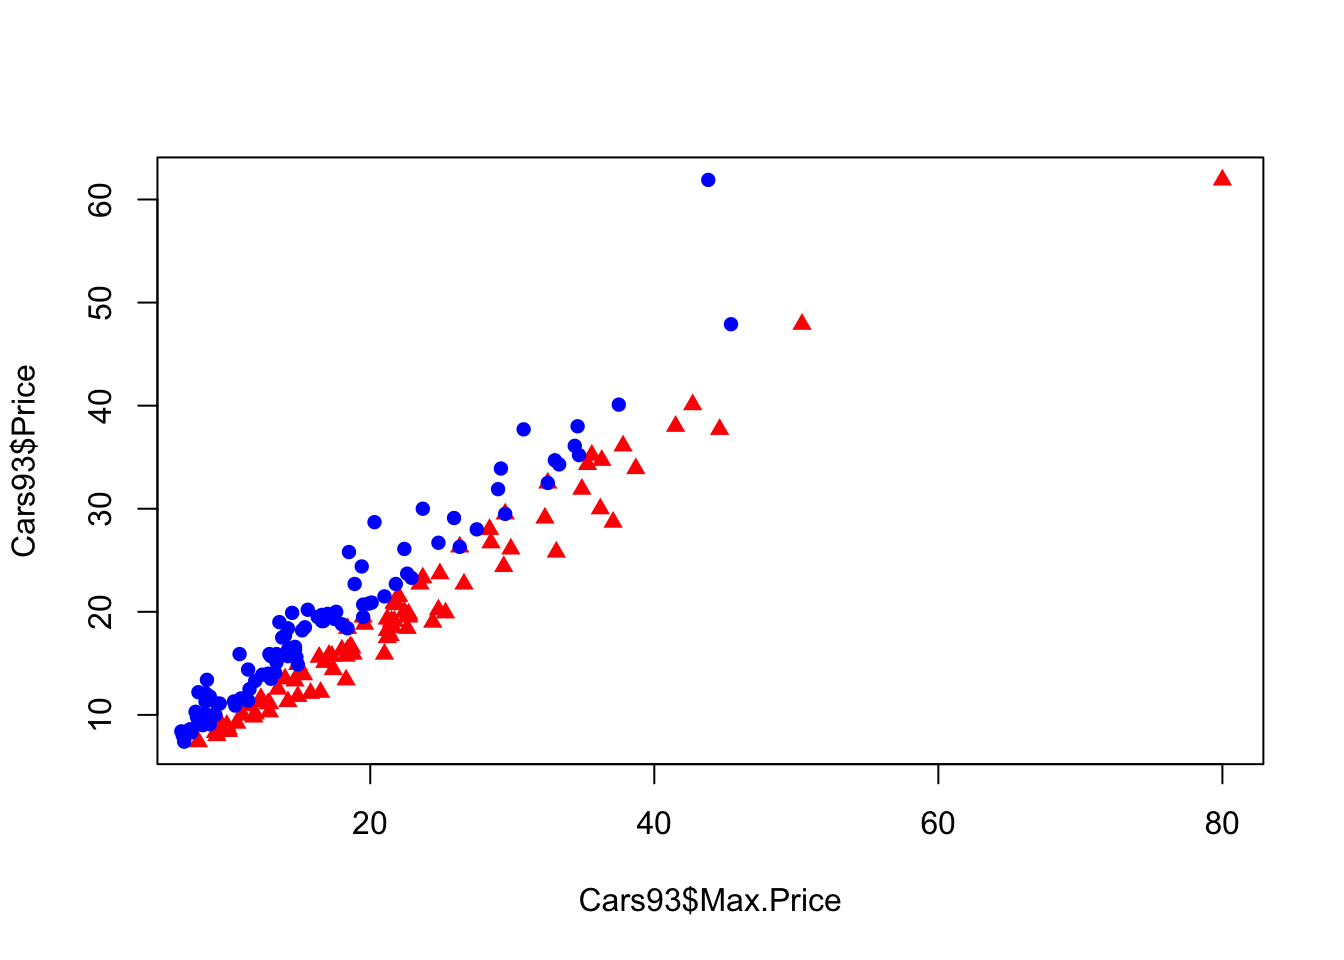
\includegraphics{bookdown-demo_files/figure-latex/unnamed-chunk-72-1.pdf}

添加一条参考线,0为截距,1为斜率,虚线

\begin{Shaded}
\begin{Highlighting}[]
\KeywordTok{plot}\NormalTok{(Cars93}\OperatorTok{$}\NormalTok{Max.Price, Cars93}\OperatorTok{$}\NormalTok{Price,}\DataTypeTok{col=}\StringTok{"red"}\NormalTok{,}\DataTypeTok{pch=}\DecValTok{17}\NormalTok{)}
\KeywordTok{points}\NormalTok{(Cars93}\OperatorTok{$}\NormalTok{Min.Price,Cars93}\OperatorTok{$}\NormalTok{Price,}\DataTypeTok{col=}\StringTok{"blue"}\NormalTok{,}\DataTypeTok{pch=}\DecValTok{16}\NormalTok{)}
\KeywordTok{abline}\NormalTok{(}\DataTypeTok{a =} \DecValTok{0}\NormalTok{, }\DataTypeTok{b =} \DecValTok{1}\NormalTok{, }\DataTypeTok{lty =} \DecValTok{2}\NormalTok{)}
\end{Highlighting}
\end{Shaded}

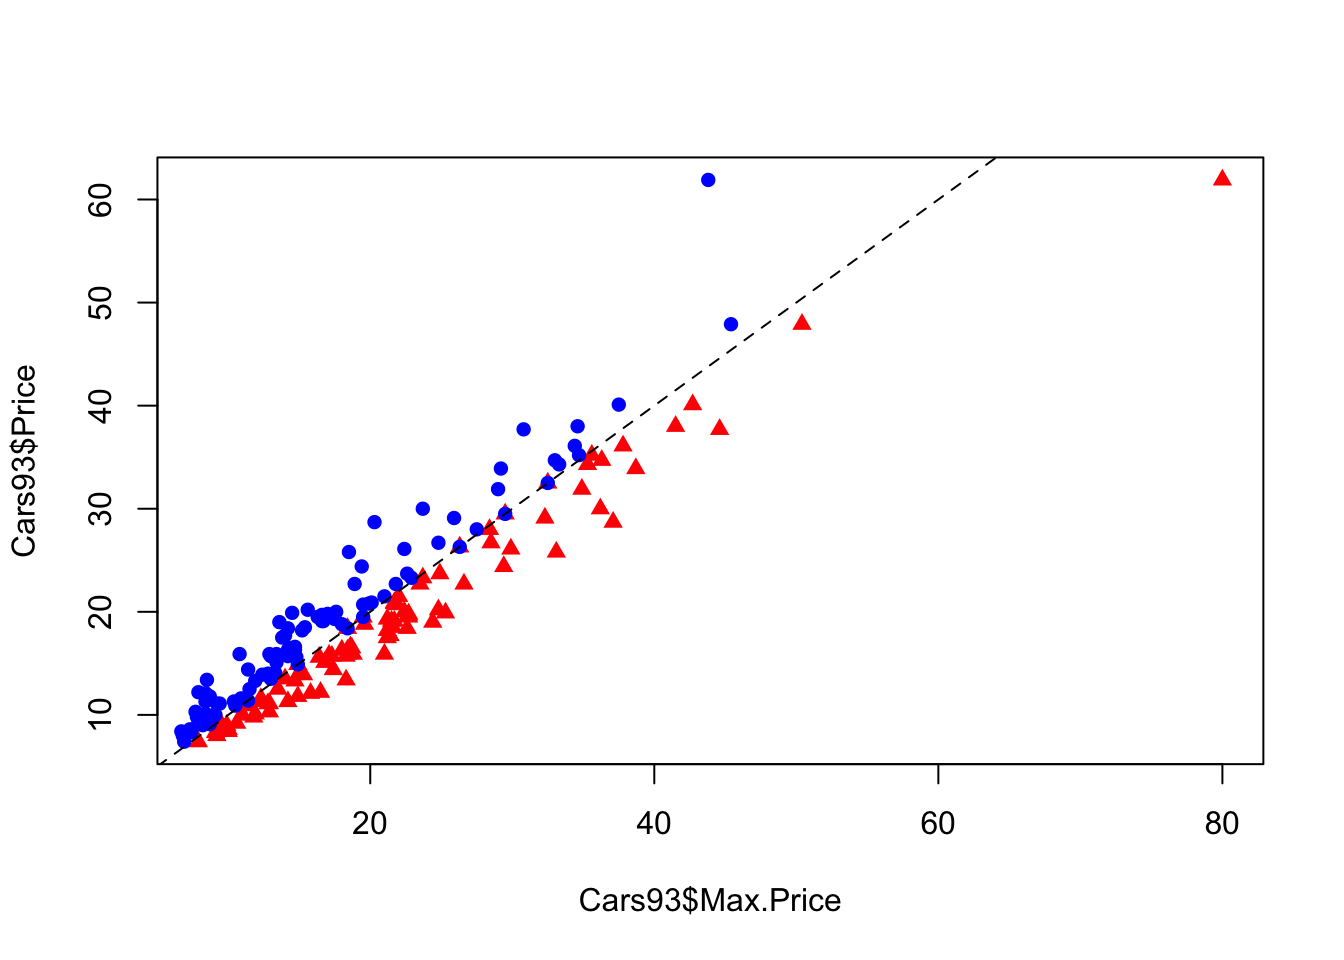
\includegraphics{bookdown-demo_files/figure-latex/unnamed-chunk-73-1.pdf}

直方图(频率图与频数图) truehist()频率直方图的函数,来自MASS这个包:

\begin{Shaded}
\begin{Highlighting}[]
\CommentTok{# Set up a side-by-side plot array}
\KeywordTok{par}\NormalTok{(}\DataTypeTok{mfrow=}\KeywordTok{c}\NormalTok{(}\DecValTok{1}\NormalTok{,}\DecValTok{2}\NormalTok{))}

\CommentTok{# Create a histogram of counts with hist()}
\KeywordTok{hist}\NormalTok{(Cars93}\OperatorTok{$}\NormalTok{Horsepower,}\DataTypeTok{main=}\StringTok{"hist() plot"}\NormalTok{)}

\CommentTok{# Create a normalized histogram with truehist()}
\KeywordTok{truehist}\NormalTok{(Cars93}\OperatorTok{$}\NormalTok{Horsepower,}\DataTypeTok{main=}\StringTok{"hist() plot"}\NormalTok{)}
\end{Highlighting}
\end{Shaded}

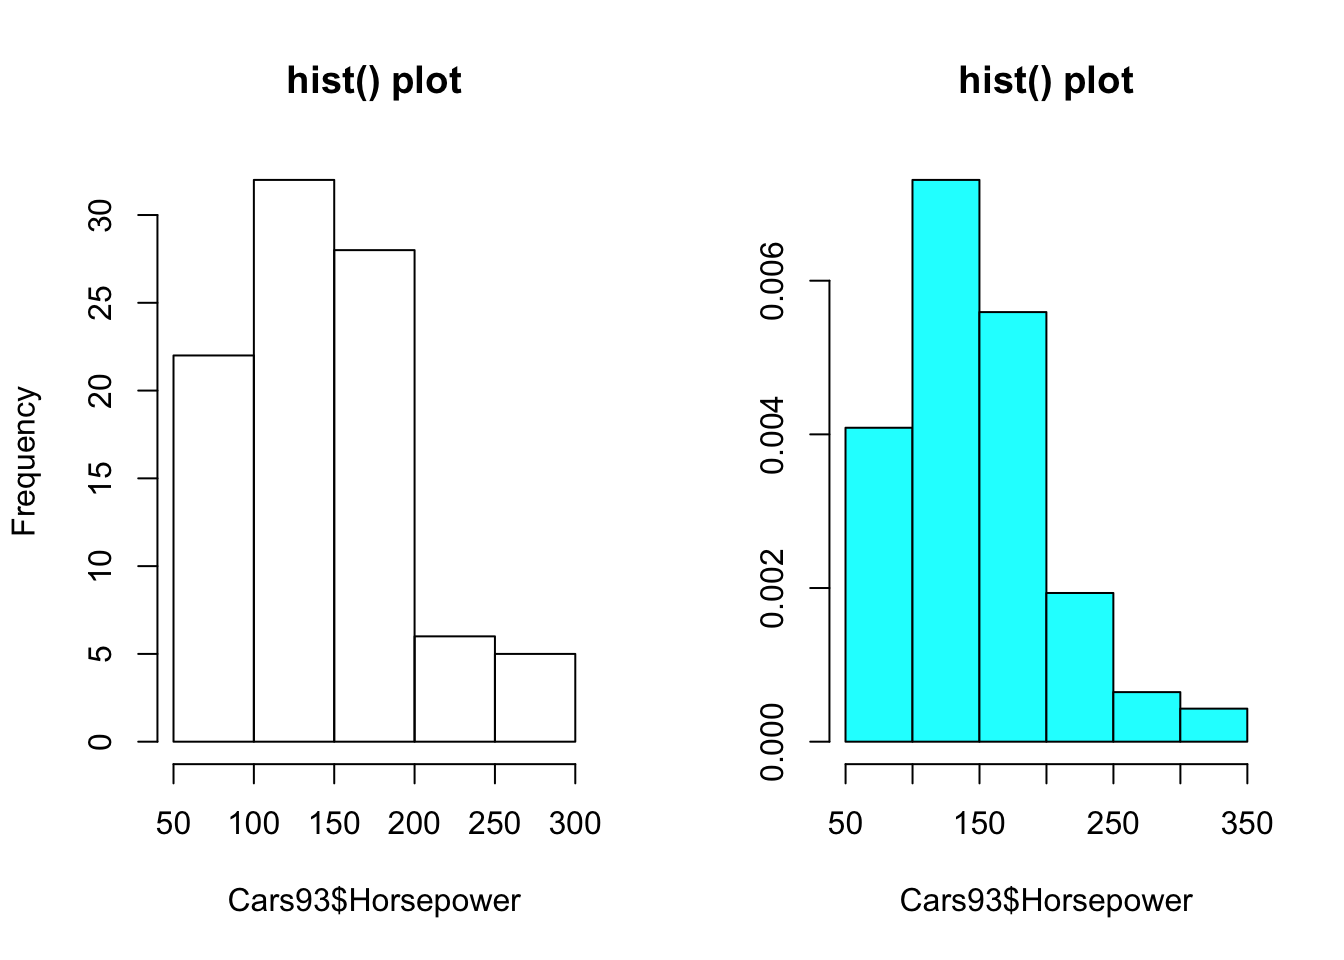
\includegraphics{bookdown-demo_files/figure-latex/unnamed-chunk-74-1.pdf}

还记得前面的鸡吗?我们来做个直方图,频率的,加一条密度曲线。

\begin{Shaded}
\begin{Highlighting}[]
\CommentTok{# Create index16, pointing to 16-week chicks}
\NormalTok{index16 <-}\StringTok{ }\KeywordTok{which}\NormalTok{(ChickWeight}\OperatorTok{$}\NormalTok{Time }\OperatorTok{==}\StringTok{ }\DecValTok{16}\NormalTok{)}

\CommentTok{# Get the 16-week chick weights}
\NormalTok{weights <-}\StringTok{ }\NormalTok{ChickWeight}\OperatorTok{$}\NormalTok{weight[index16]}

\CommentTok{# Plot the normalized histogram}
\KeywordTok{truehist}\NormalTok{(weights)}

\CommentTok{# Add the density curve to the histogram}
\KeywordTok{lines}\NormalTok{(}\KeywordTok{density}\NormalTok{(weights))}
\end{Highlighting}
\end{Shaded}

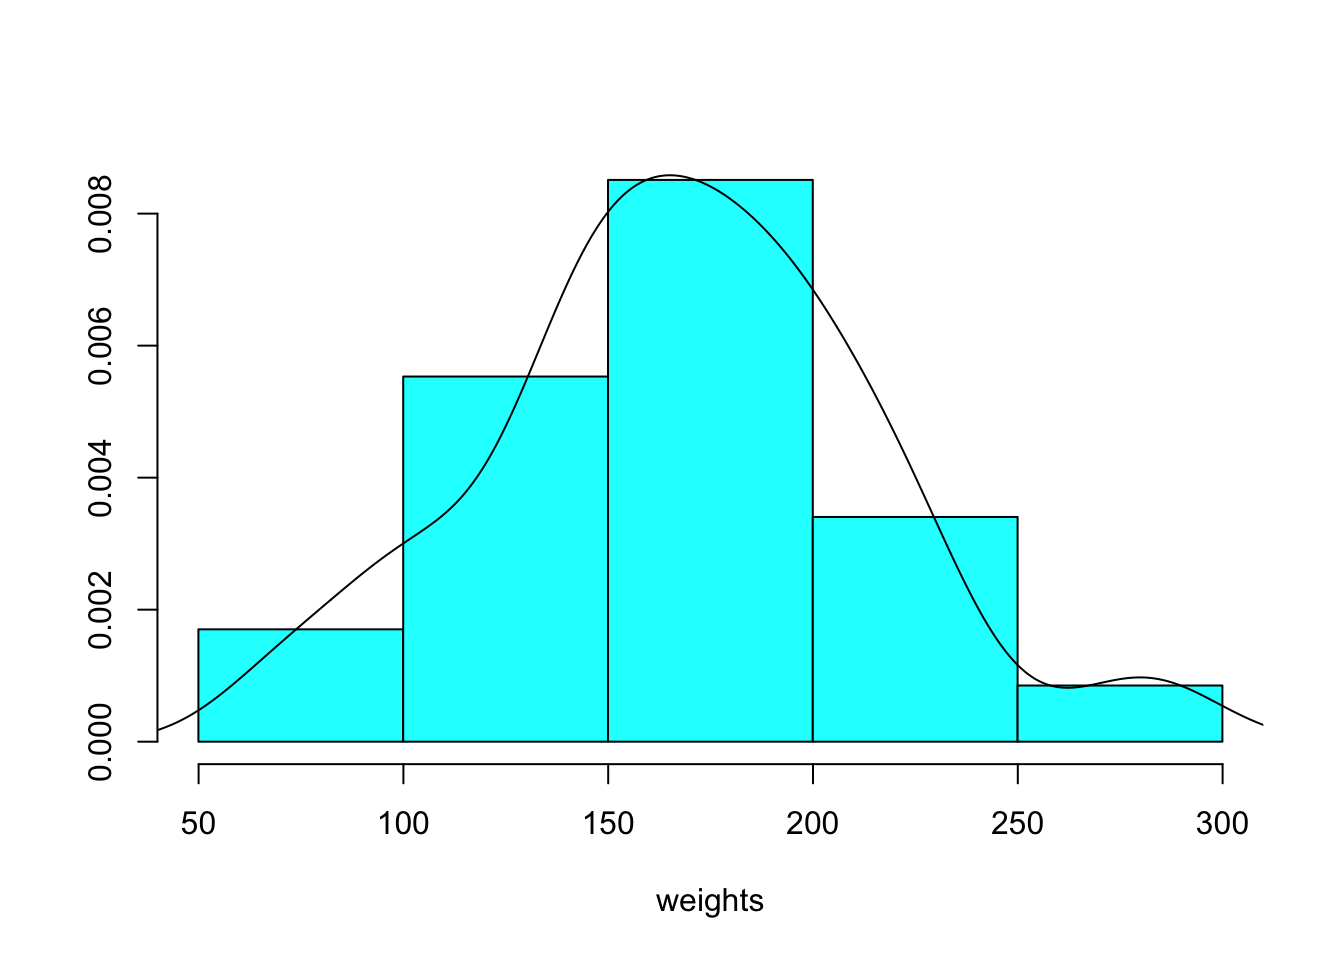
\includegraphics{bookdown-demo_files/figure-latex/unnamed-chunk-75-1.pdf}

使用\texttt{par()}在一个面板上画出多幅图并可修改细节:

\begin{Shaded}
\begin{Highlighting}[]
\KeywordTok{par}\NormalTok{(}\StringTok{"bg"}\NormalTok{) }\CommentTok{#背景颜色,默认白色}
\end{Highlighting}
\end{Shaded}

\begin{verbatim}
## [1] "transparent"
\end{verbatim}

\begin{Shaded}
\begin{Highlighting}[]
\KeywordTok{par}\NormalTok{(}\StringTok{"col"}\NormalTok{) }\CommentTok{# 作图颜色,默认黑色}
\end{Highlighting}
\end{Shaded}

\begin{verbatim}
## [1] "black"
\end{verbatim}

\begin{Shaded}
\begin{Highlighting}[]
\KeywordTok{par}\NormalTok{(}\StringTok{"mar"}\NormalTok{) }\CommentTok{#(bottom, left, top, right) 图片边距}
\end{Highlighting}
\end{Shaded}

\begin{verbatim}
## [1] 5.1 4.1 4.1 2.1
\end{verbatim}

\begin{Shaded}
\begin{Highlighting}[]
\KeywordTok{par}\NormalTok{(}\StringTok{"mfrow"}\NormalTok{) }\CommentTok{#默认一行一列}
\end{Highlighting}
\end{Shaded}

\begin{verbatim}
## [1] 1 1
\end{verbatim}

\begin{Shaded}
\begin{Highlighting}[]
\NormalTok{?par}
\end{Highlighting}
\end{Shaded}

\begin{Shaded}
\begin{Highlighting}[]
\CommentTok{#通过改变全局参数,使面板中呈现多幅图片}
\KeywordTok{par}\NormalTok{(}\DataTypeTok{mfrow =} \KeywordTok{c}\NormalTok{(}\DecValTok{2}\NormalTok{,}\DecValTok{2}\NormalTok{)) }\CommentTok{#设置成2行两列}
\KeywordTok{hist}\NormalTok{(airquality}\OperatorTok{$}\NormalTok{Temp)}
\KeywordTok{hist}\NormalTok{(airquality}\OperatorTok{$}\NormalTok{Temp, }\DataTypeTok{freq =} \OtherTok{FALSE}\NormalTok{)}
\KeywordTok{hist}\NormalTok{(airquality}\OperatorTok{$}\NormalTok{Temp, }\DataTypeTok{freq =} \OtherTok{FALSE}\NormalTok{, }\DataTypeTok{col=}\StringTok{"blue"}\NormalTok{)}

\KeywordTok{hist}\NormalTok{(airquality}\OperatorTok{$}\NormalTok{Temp, }\DataTypeTok{freq =} \OtherTok{FALSE}\NormalTok{, }\DataTypeTok{col=}\StringTok{"blue"}\NormalTok{)}
\KeywordTok{lines}\NormalTok{(}\KeywordTok{density}\NormalTok{(airquality}\OperatorTok{$}\NormalTok{Temp))}
\end{Highlighting}
\end{Shaded}

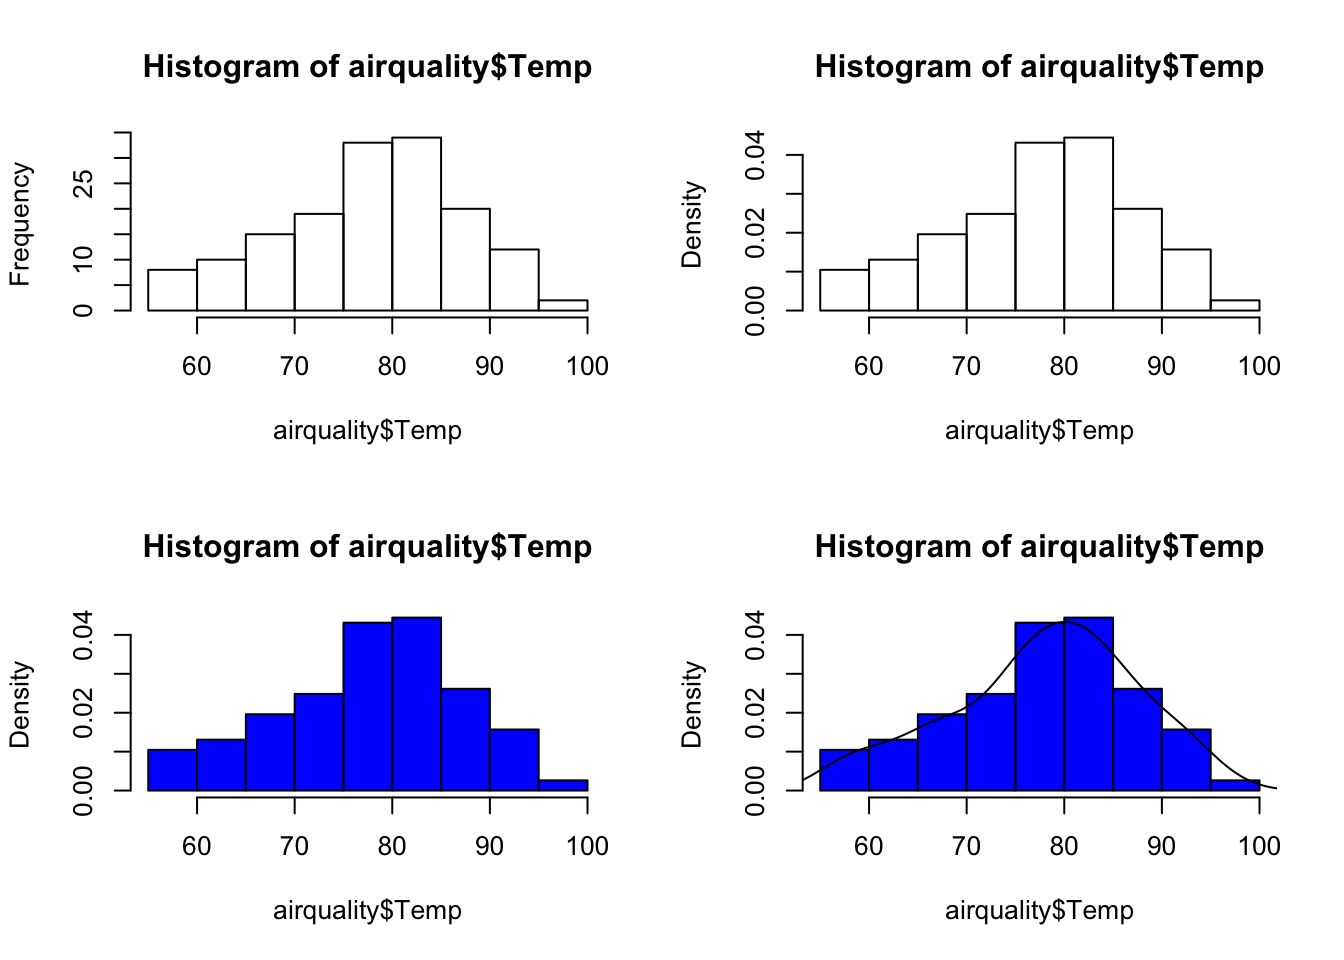
\includegraphics{bookdown-demo_files/figure-latex/unnamed-chunk-77-1.pdf}

\begin{Shaded}
\begin{Highlighting}[]
\KeywordTok{par}\NormalTok{(}\DataTypeTok{mfrow =} \KeywordTok{c}\NormalTok{(}\DecValTok{1}\NormalTok{,}\DecValTok{1}\NormalTok{))}
\KeywordTok{truehist}\NormalTok{(airquality}\OperatorTok{$}\NormalTok{Temp)}
\KeywordTok{lines}\NormalTok{(}\KeywordTok{density}\NormalTok{(airquality}\OperatorTok{$}\NormalTok{Temp))}
\end{Highlighting}
\end{Shaded}

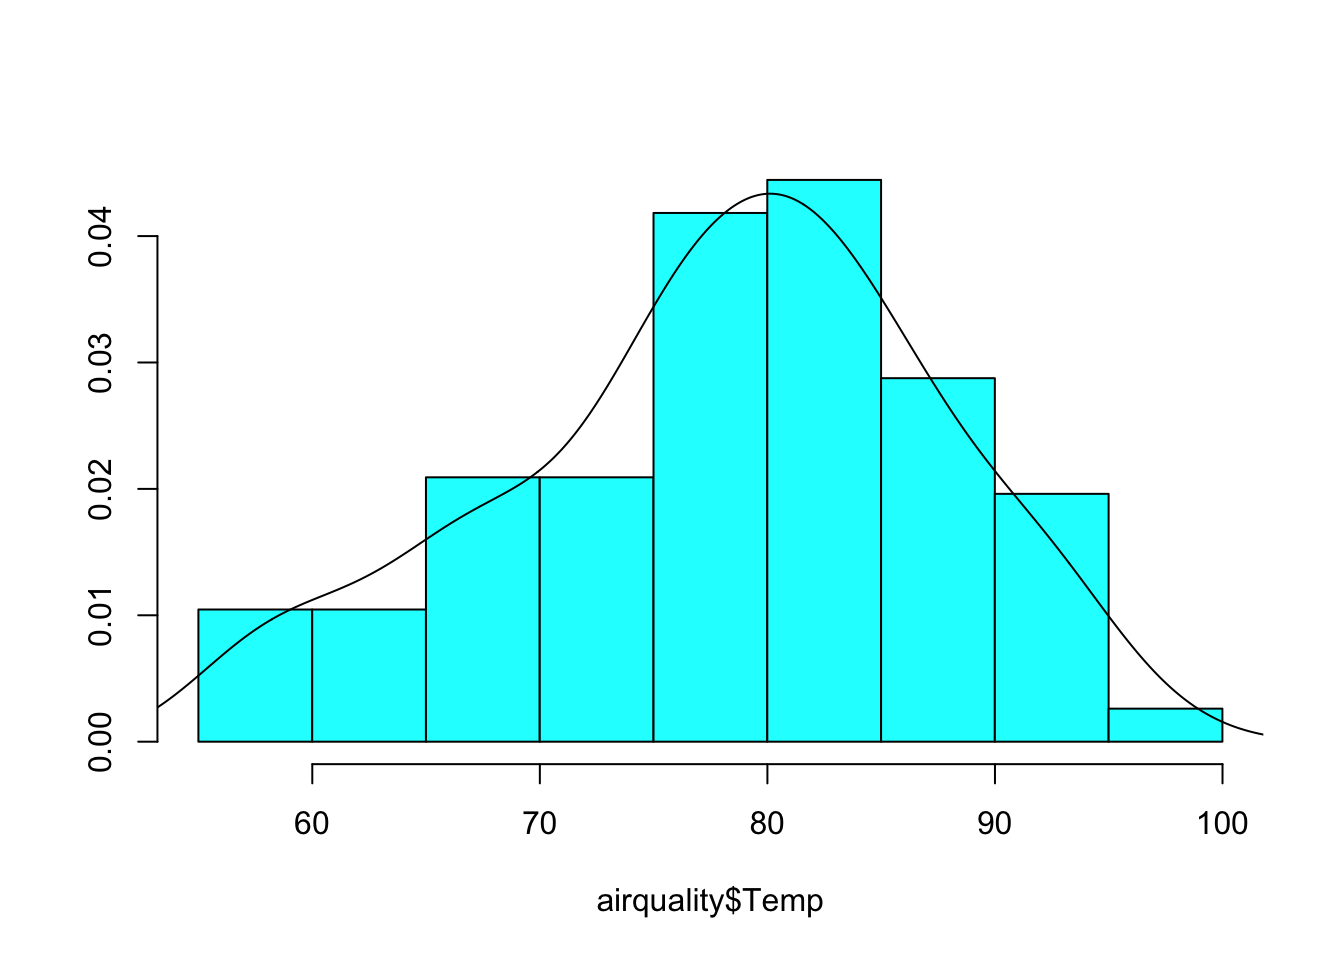
\includegraphics{bookdown-demo_files/figure-latex/unnamed-chunk-77-2.pdf}

散点图中的菊花图,让你更懂数据

\begin{Shaded}
\begin{Highlighting}[]
\CommentTok{# Set up a side-by-side plot array}
\KeywordTok{par}\NormalTok{(}\DataTypeTok{mfrow=}\KeywordTok{c}\NormalTok{(}\DecValTok{1}\NormalTok{,}\DecValTok{2}\NormalTok{))}

\CommentTok{# Create the standard scatterplot}
\KeywordTok{plot}\NormalTok{(rad}\OperatorTok{~}\NormalTok{zn,}\DataTypeTok{data=}\NormalTok{Boston)}

\CommentTok{# Add the title}
\KeywordTok{title}\NormalTok{(}\StringTok{"Standard scatterplot"}\NormalTok{)}

\CommentTok{# Create the sunflowerplot}
\KeywordTok{sunflowerplot}\NormalTok{(rad}\OperatorTok{~}\NormalTok{zn,}\DataTypeTok{data=}\NormalTok{Boston)}

\CommentTok{# Add the title}
\KeywordTok{title}\NormalTok{(}\StringTok{"Sunflower plot"}\NormalTok{)}
\end{Highlighting}
\end{Shaded}

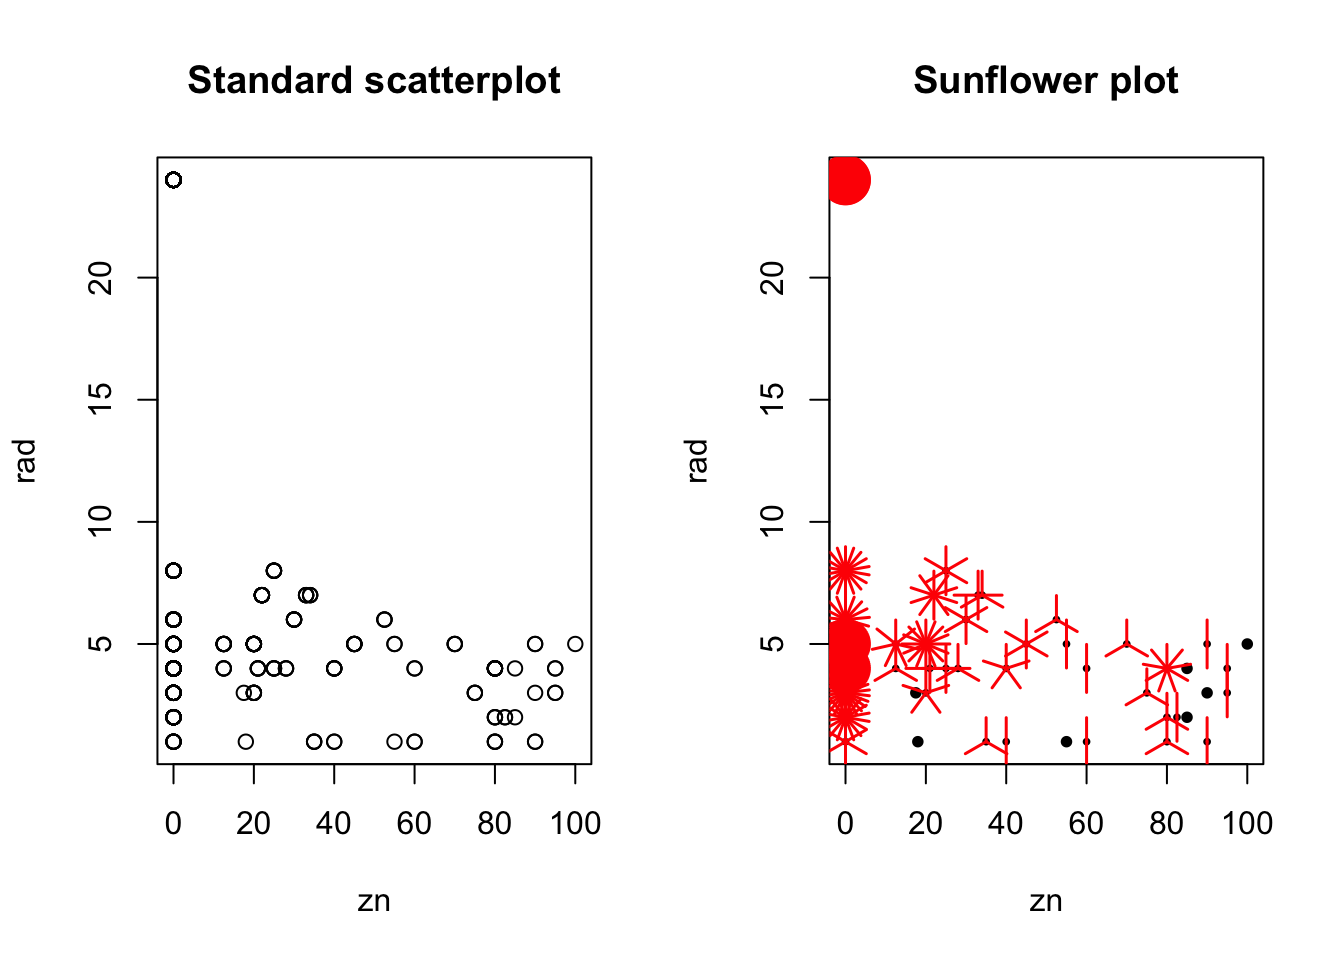
\includegraphics{bookdown-demo_files/figure-latex/unnamed-chunk-78-1.pdf}

\begin{Shaded}
\begin{Highlighting}[]
\CommentTok{#按月份,给每一个月的温度绘箱图}
\CommentTok{#month是分类变量}
\KeywordTok{boxplot}\NormalTok{(Temp}\OperatorTok{~}\NormalTok{Month,airquality,}\DataTypeTok{xlab=}\StringTok{"month"}\NormalTok{, }
        \DataTypeTok{ylab=}\StringTok{"Temperature (F)"}\NormalTok{)}
\end{Highlighting}
\end{Shaded}

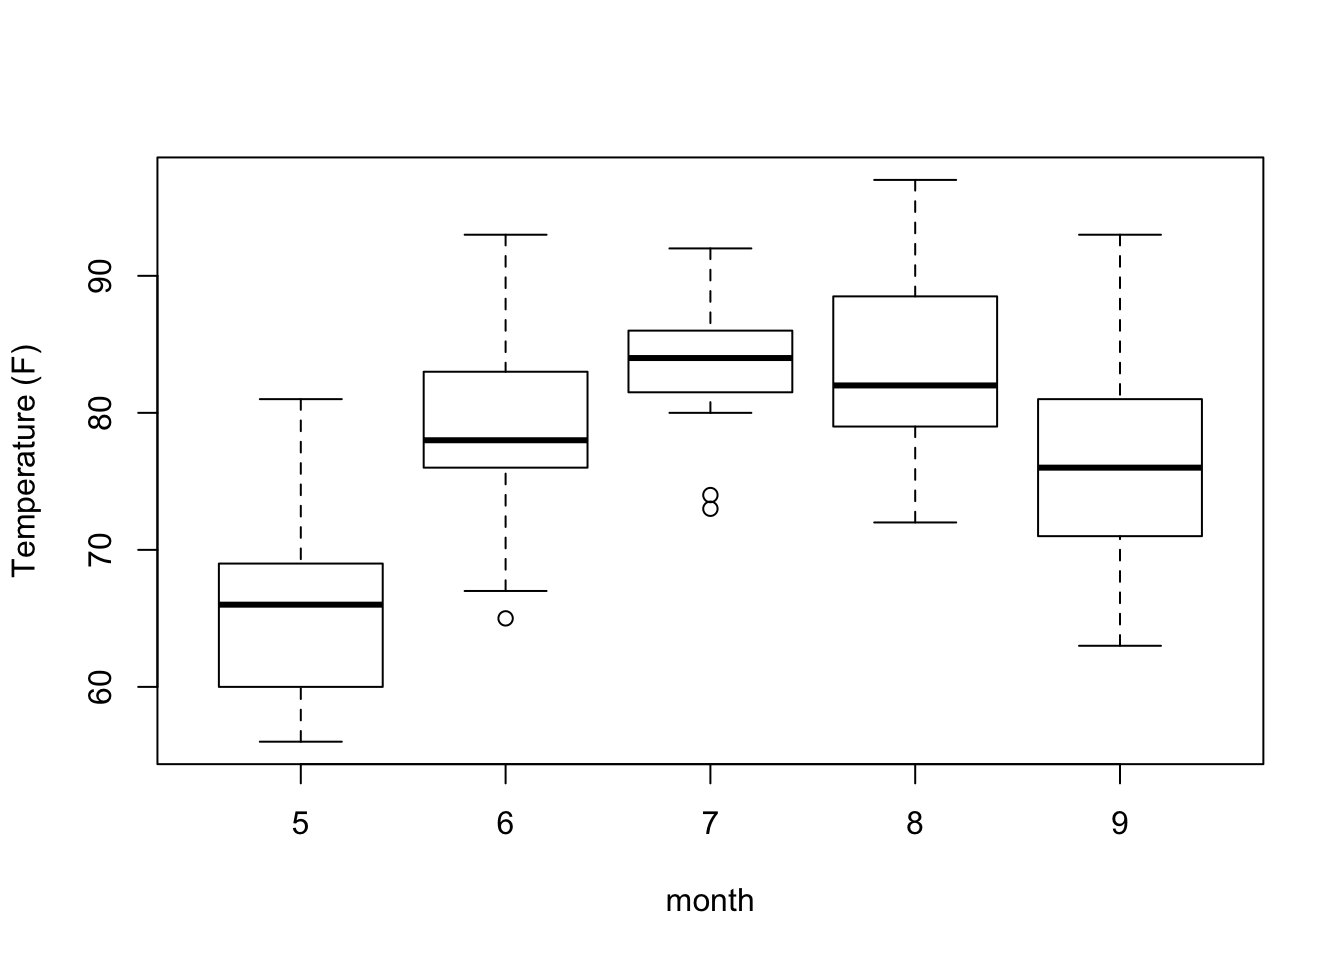
\includegraphics{bookdown-demo_files/figure-latex/unnamed-chunk-79-1.pdf}

\begin{Shaded}
\begin{Highlighting}[]
\CommentTok{#with() 更简便的绘图函数,}
\CommentTok{# 再不用每个变量都引用数据集}
\KeywordTok{with}\NormalTok{(airquality, }\KeywordTok{plot}\NormalTok{(Wind}\OperatorTok{~}\NormalTok{Temp))}
\KeywordTok{title}\NormalTok{(}\DataTypeTok{main=}\StringTok{"wind and temp in NYC"}\NormalTok{) }\CommentTok{#使用title进行修饰}
\end{Highlighting}
\end{Shaded}

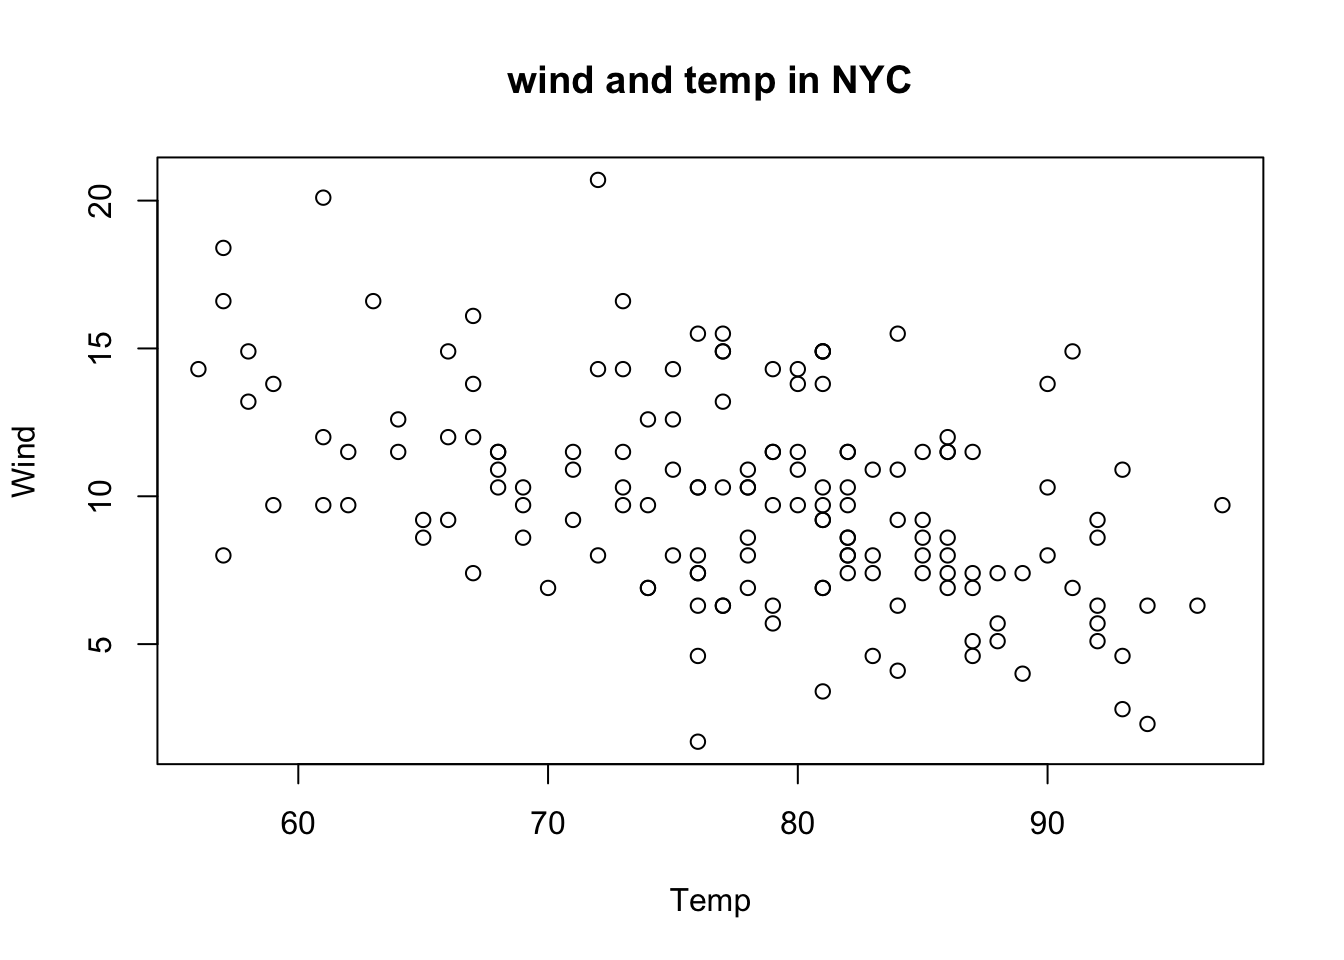
\includegraphics{bookdown-demo_files/figure-latex/unnamed-chunk-80-1.pdf}

\begin{Shaded}
\begin{Highlighting}[]
\CommentTok{#另外一种方式添加标题,一样的结果}
\KeywordTok{with}\NormalTok{(airquality, }\KeywordTok{plot}\NormalTok{(Wind, Temp,}
     \DataTypeTok{main=}\StringTok{"wind and temp in NYC"}\NormalTok{)) }
\end{Highlighting}
\end{Shaded}

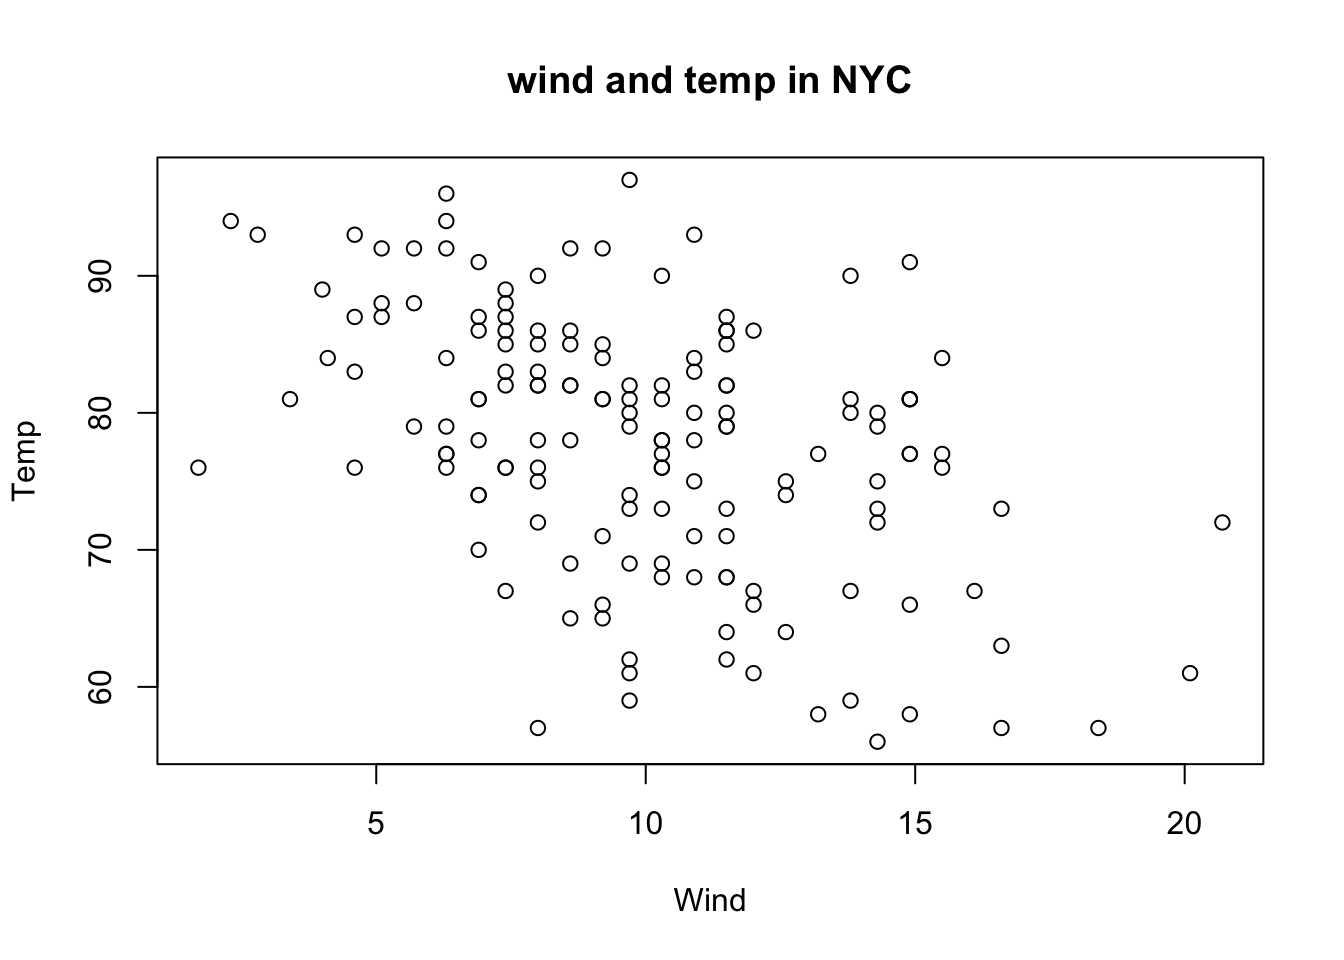
\includegraphics{bookdown-demo_files/figure-latex/unnamed-chunk-81-1.pdf}

\begin{Shaded}
\begin{Highlighting}[]
\CommentTok{#有用的 type="n"}
\KeywordTok{with}\NormalTok{(airquality, }\KeywordTok{plot}\NormalTok{(Wind, Temp,}
                      \DataTypeTok{main=}\StringTok{"Wind and Temp in NYC"}\NormalTok{,}
                      \DataTypeTok{type=}\StringTok{"n"}\NormalTok{))}
\end{Highlighting}
\end{Shaded}

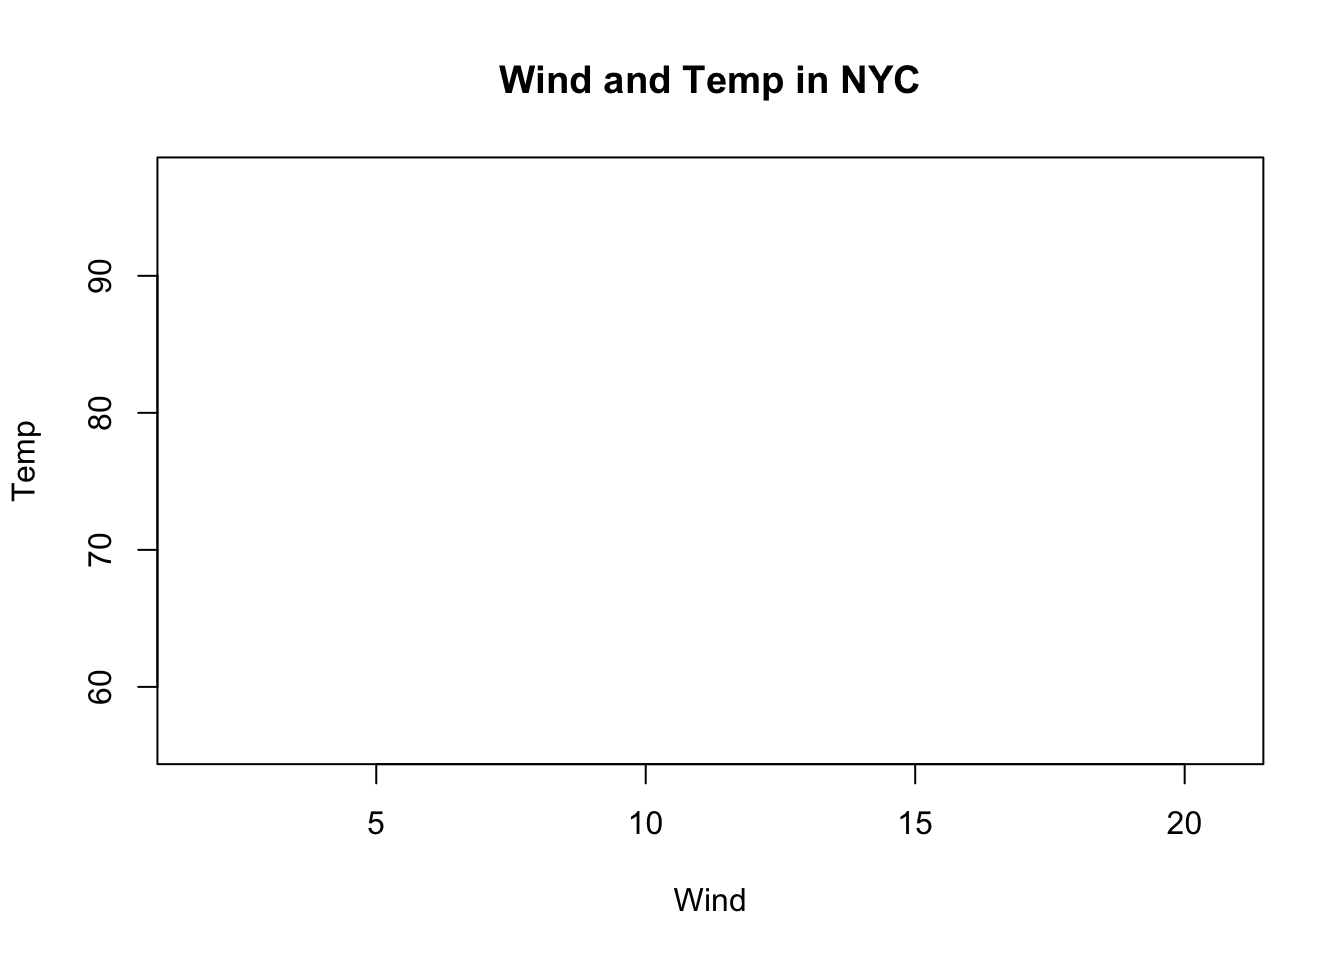
\includegraphics{bookdown-demo_files/figure-latex/unnamed-chunk-82-1.pdf}

\begin{Shaded}
\begin{Highlighting}[]
\KeywordTok{with}\NormalTok{(airquality, }\KeywordTok{plot}\NormalTok{(Wind, Temp,}
                      \DataTypeTok{main=}\StringTok{"Wind and Temp in NYC"}\NormalTok{,}
                      \DataTypeTok{type=}\StringTok{"n"}\NormalTok{))}
\KeywordTok{with}\NormalTok{(}\KeywordTok{subset}\NormalTok{(airquality, Month}\OperatorTok{==}\DecValTok{9}\NormalTok{), }
     \KeywordTok{points}\NormalTok{(Wind, Temp, }\DataTypeTok{col=}\StringTok{"red"}\NormalTok{))}
\end{Highlighting}
\end{Shaded}

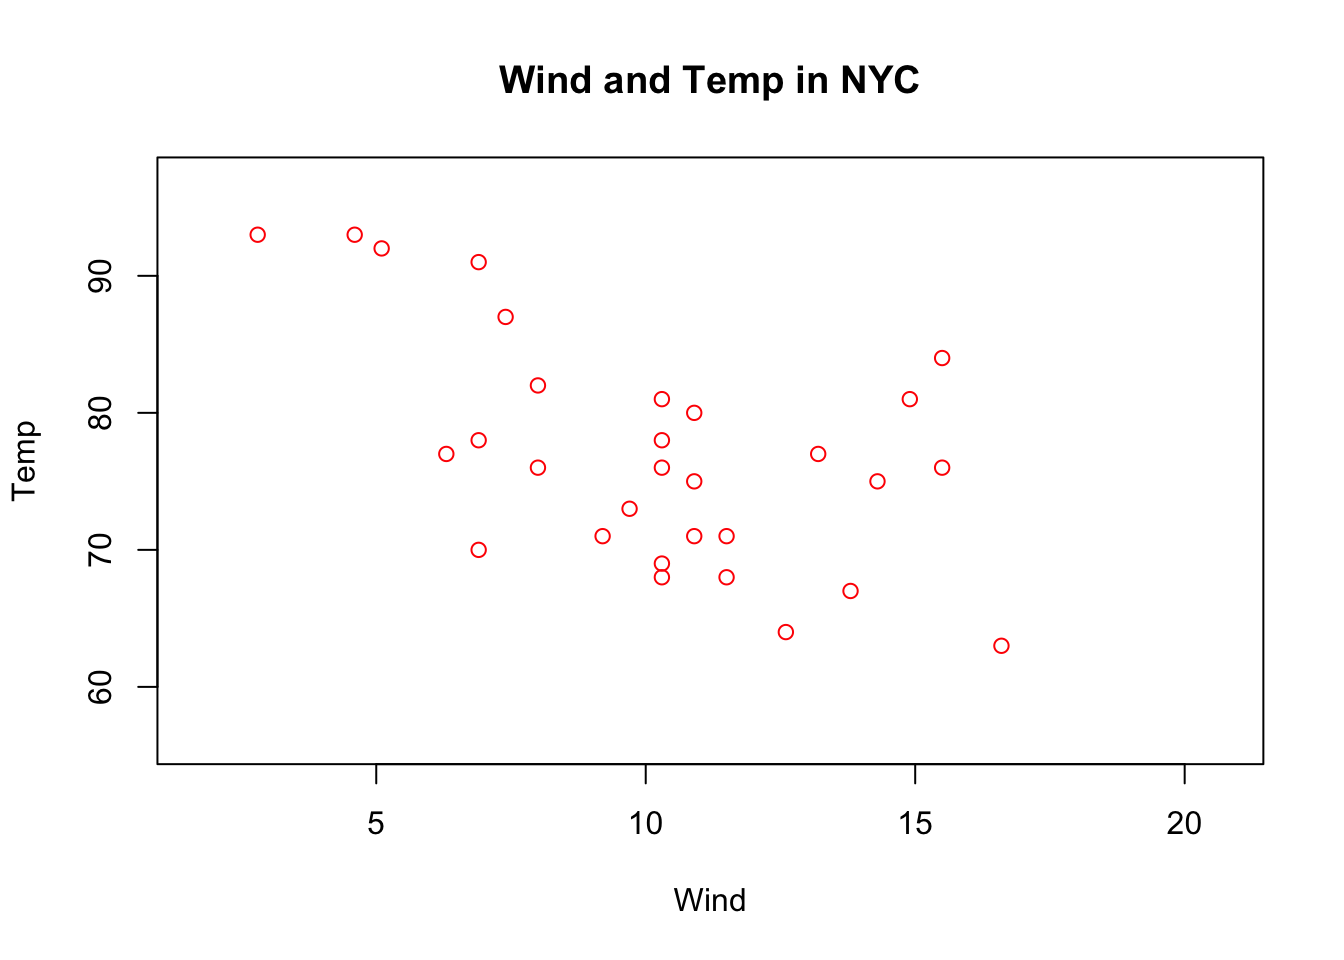
\includegraphics{bookdown-demo_files/figure-latex/unnamed-chunk-83-1.pdf}

\begin{Shaded}
\begin{Highlighting}[]
\KeywordTok{with}\NormalTok{(airquality, }\KeywordTok{plot}\NormalTok{(Wind, Temp,}
                      \DataTypeTok{main=}\StringTok{"Wind and Temp in NYC"}\NormalTok{,}
                      \DataTypeTok{type=}\StringTok{"n"}\NormalTok{))}
\KeywordTok{with}\NormalTok{(}\KeywordTok{subset}\NormalTok{(airquality, Month}\OperatorTok{==}\DecValTok{9}\NormalTok{), }
     \KeywordTok{points}\NormalTok{(Wind, Temp, }\DataTypeTok{col=}\StringTok{"red"}\NormalTok{))}
\KeywordTok{with}\NormalTok{(}\KeywordTok{subset}\NormalTok{(airquality, Month}\OperatorTok{==}\DecValTok{8}\NormalTok{), }
     \KeywordTok{points}\NormalTok{(Wind, Temp, }\DataTypeTok{col=}\StringTok{"blue"}\NormalTok{))}
\end{Highlighting}
\end{Shaded}

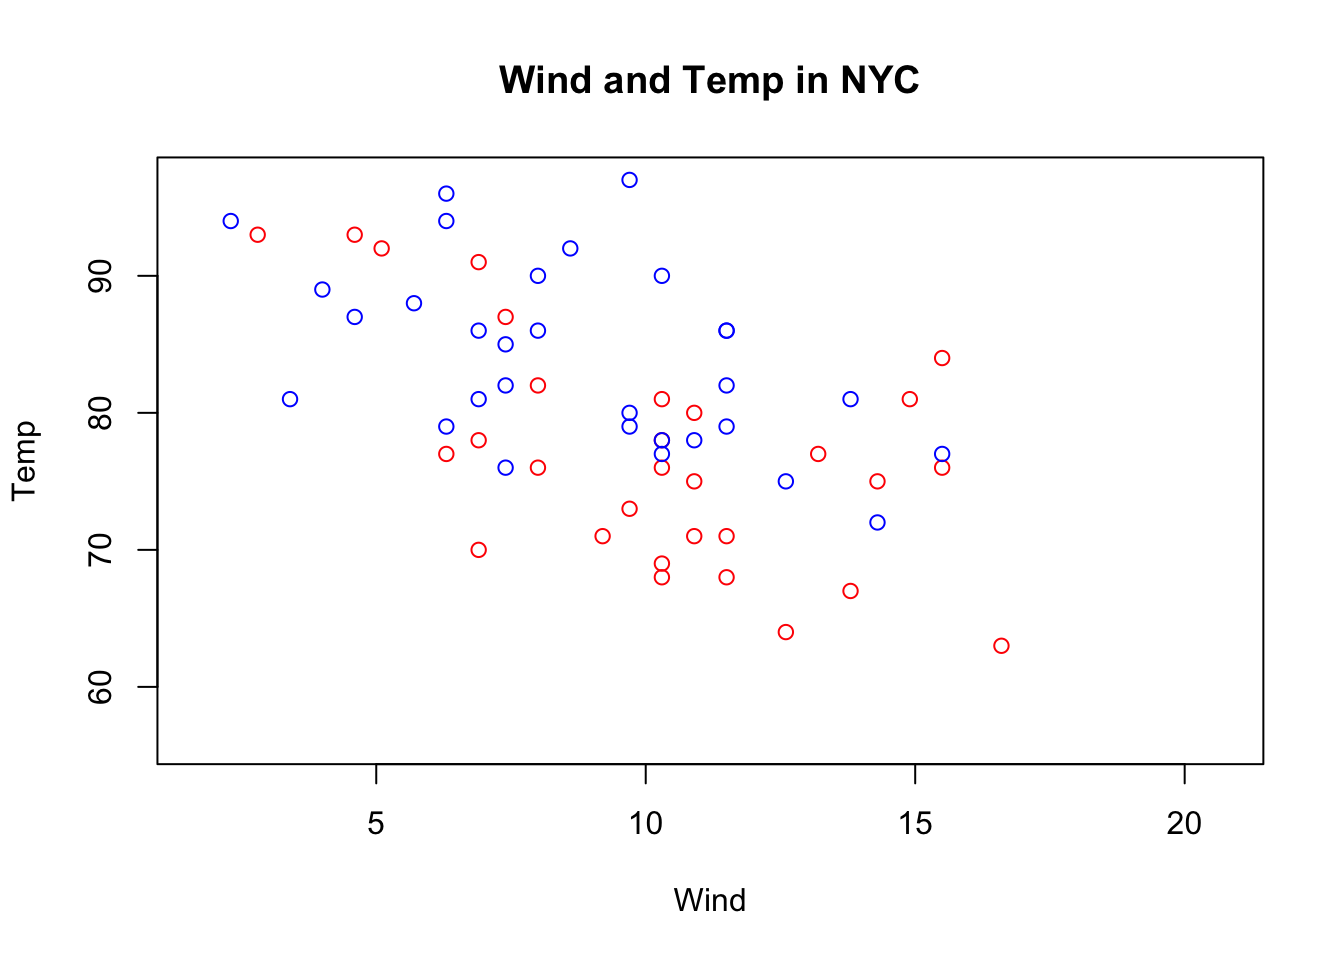
\includegraphics{bookdown-demo_files/figure-latex/unnamed-chunk-84-1.pdf}

\begin{Shaded}
\begin{Highlighting}[]
\KeywordTok{with}\NormalTok{(airquality, }\KeywordTok{plot}\NormalTok{(Wind, Temp,}
                      \DataTypeTok{main=}\StringTok{"Wind and Temp in NYC"}\NormalTok{,}
                      \DataTypeTok{type=}\StringTok{"n"}\NormalTok{))}
\KeywordTok{with}\NormalTok{(}\KeywordTok{subset}\NormalTok{(airquality, Month}\OperatorTok{==}\DecValTok{9}\NormalTok{), }
     \KeywordTok{points}\NormalTok{(Wind, Temp, }\DataTypeTok{col=}\StringTok{"red"}\NormalTok{))}

\KeywordTok{with}\NormalTok{(}\KeywordTok{subset}\NormalTok{(airquality, Month}\OperatorTok{==}\DecValTok{8}\NormalTok{), }
     \KeywordTok{points}\NormalTok{(Wind, Temp, }\DataTypeTok{col=}\StringTok{"blue"}\NormalTok{))}

\KeywordTok{with}\NormalTok{(}\KeywordTok{subset}\NormalTok{(airquality, Month}\OperatorTok{==}\DecValTok{7}\NormalTok{), }
     \KeywordTok{points}\NormalTok{(Wind, Temp, }\DataTypeTok{col=}\StringTok{"green"}\NormalTok{))}
\end{Highlighting}
\end{Shaded}

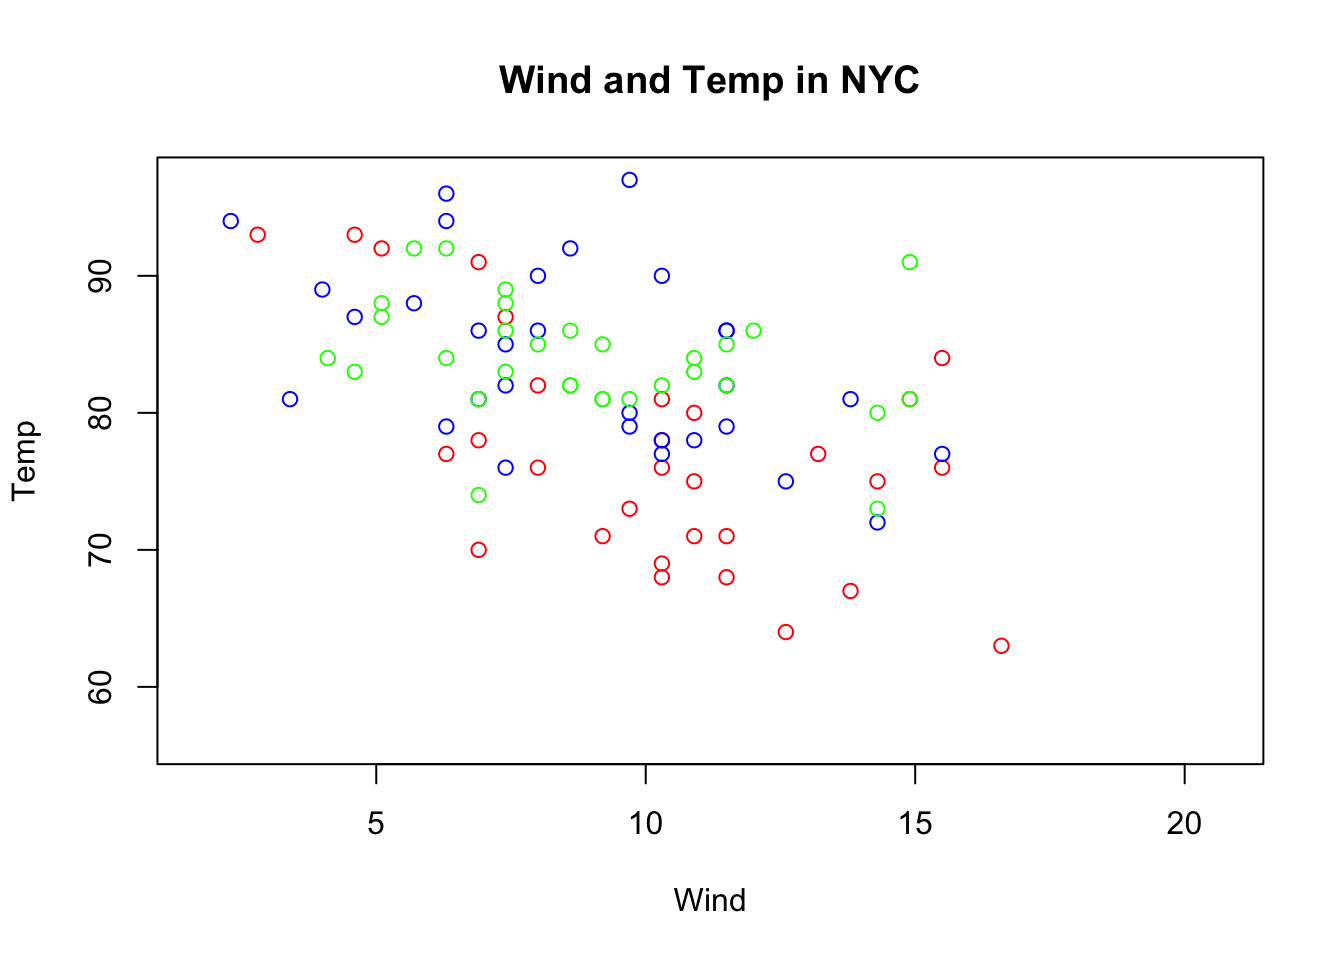
\includegraphics{bookdown-demo_files/figure-latex/unnamed-chunk-85-1.pdf}

\begin{Shaded}
\begin{Highlighting}[]
\CommentTok{#完成了用不同的颜色表示不同的月份的点}
\end{Highlighting}
\end{Shaded}

\begin{Shaded}
\begin{Highlighting}[]
\KeywordTok{with}\NormalTok{(airquality, }\KeywordTok{plot}\NormalTok{(Wind, Temp,}
                      \DataTypeTok{main=}\StringTok{"Wind and Temp in NYC"}\NormalTok{,}
                      \DataTypeTok{type=}\StringTok{"n"}\NormalTok{))}
\KeywordTok{with}\NormalTok{(}\KeywordTok{subset}\NormalTok{(airquality, Month}\OperatorTok{==}\DecValTok{9}\NormalTok{), }
     \KeywordTok{points}\NormalTok{(Wind, Temp, }\DataTypeTok{col=}\StringTok{"red"}\NormalTok{))}

\KeywordTok{with}\NormalTok{(}\KeywordTok{subset}\NormalTok{(airquality, Month}\OperatorTok{==}\DecValTok{8}\NormalTok{), }
     \KeywordTok{points}\NormalTok{(Wind, Temp, }\DataTypeTok{col=}\StringTok{"blue"}\NormalTok{))}

\KeywordTok{with}\NormalTok{(}\KeywordTok{subset}\NormalTok{(airquality, Month}\OperatorTok{==}\DecValTok{7}\NormalTok{), }
     \KeywordTok{points}\NormalTok{(Wind, Temp, }\DataTypeTok{col=}\StringTok{"green"}\NormalTok{))}

\KeywordTok{with}\NormalTok{(}\KeywordTok{subset}\NormalTok{(airquality, Month }\OperatorTok\StringTok{ }\KeywordTok{c}\NormalTok{(}\DecValTok{5}\NormalTok{,}\DecValTok{6}\NormalTok{)), }
     \KeywordTok{points}\NormalTok{(Wind, Temp, }\DataTypeTok{col=}\StringTok{"black"}\NormalTok{))}
\end{Highlighting}
\end{Shaded}

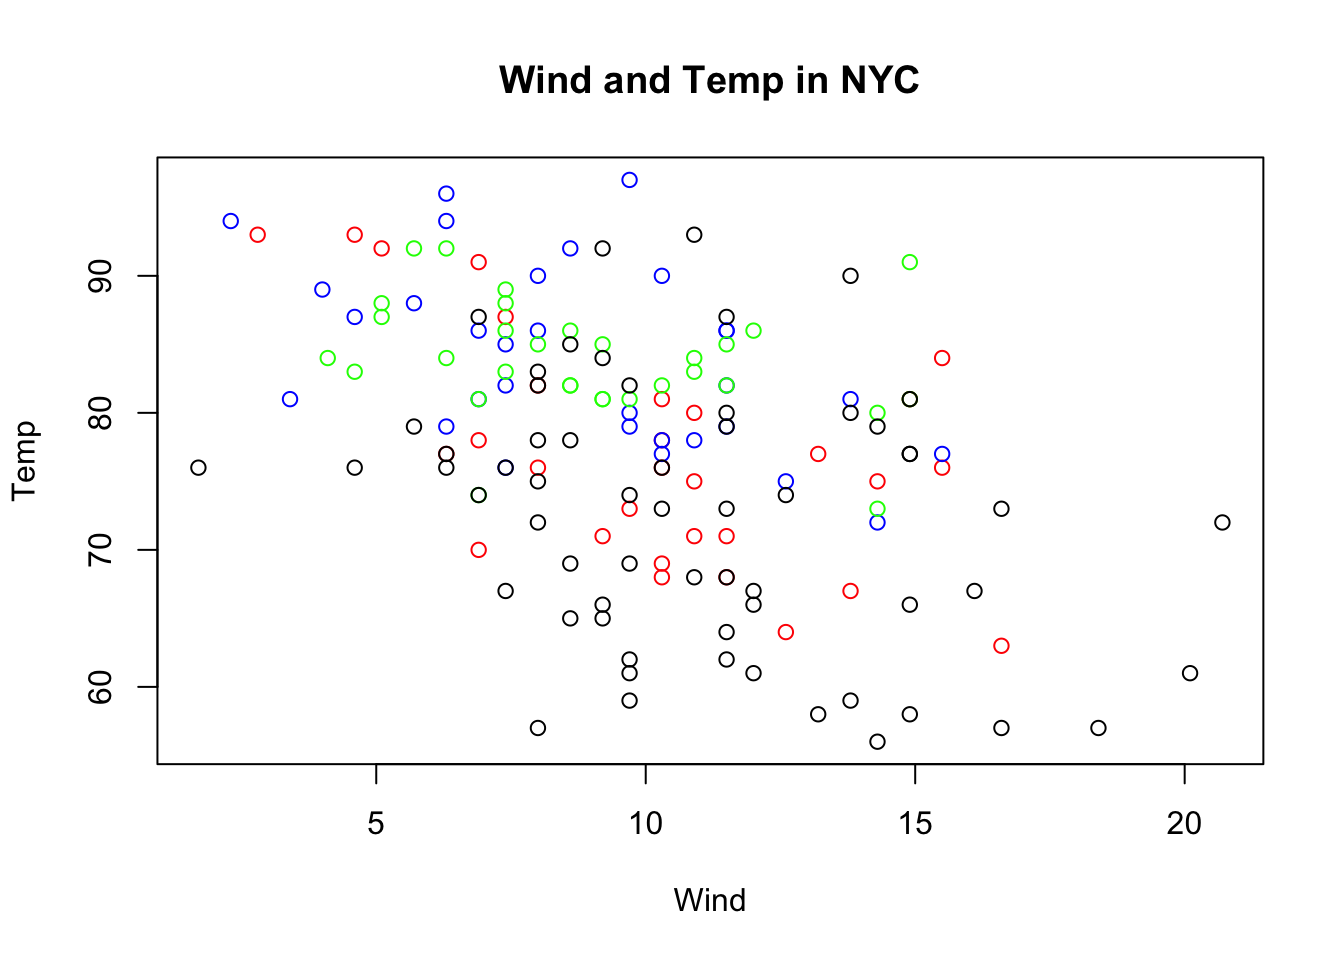
\includegraphics{bookdown-demo_files/figure-latex/unnamed-chunk-86-1.pdf}

\begin{Shaded}
\begin{Highlighting}[]
\KeywordTok{with}\NormalTok{(airquality, }\KeywordTok{plot}\NormalTok{(Wind, Temp,}
                      \DataTypeTok{main=}\StringTok{"Wind and Temp in NYC"}\NormalTok{,}
                      \DataTypeTok{type=}\StringTok{"n"}\NormalTok{))}
\KeywordTok{with}\NormalTok{(}\KeywordTok{subset}\NormalTok{(airquality, Month}\OperatorTok{==}\DecValTok{9}\NormalTok{), }
     \KeywordTok{points}\NormalTok{(Wind, Temp, }\DataTypeTok{col=}\StringTok{"red"}\NormalTok{))}

\KeywordTok{with}\NormalTok{(}\KeywordTok{subset}\NormalTok{(airquality, Month}\OperatorTok{==}\DecValTok{8}\NormalTok{), }
     \KeywordTok{points}\NormalTok{(Wind, Temp, }\DataTypeTok{col=}\StringTok{"blue"}\NormalTok{))}

\KeywordTok{with}\NormalTok{(}\KeywordTok{subset}\NormalTok{(airquality, Month}\OperatorTok{==}\DecValTok{7}\NormalTok{), }
     \KeywordTok{points}\NormalTok{(Wind, Temp, }\DataTypeTok{col=}\StringTok{"green"}\NormalTok{))}

\KeywordTok{with}\NormalTok{(}\KeywordTok{subset}\NormalTok{(airquality, Month }\OperatorTok\StringTok{ }\KeywordTok{c}\NormalTok{(}\DecValTok{5}\NormalTok{,}\DecValTok{6}\NormalTok{)), }
     \KeywordTok{points}\NormalTok{(Wind, Temp, }\DataTypeTok{col=}\StringTok{"black"}\NormalTok{))}

\NormalTok{fit<-}\KeywordTok{lm}\NormalTok{(Temp}\OperatorTok{~}\NormalTok{Wind, airquality) }\CommentTok{#拟合一个回归模型}
\KeywordTok{abline}\NormalTok{(fit,}\DataTypeTok{lwd=}\DecValTok{2}\NormalTok{) }\CommentTok{#把回归线加进去}

\CommentTok{#加入图例,说明颜色含义}
\KeywordTok{legend}\NormalTok{(}\StringTok{"topright"}\NormalTok{, }\DataTypeTok{pch=}\DecValTok{1}\NormalTok{, }\CommentTok{#右上角,空心圆点}
       \DataTypeTok{col=}\KeywordTok{c}\NormalTok{(}\StringTok{"red"}\NormalTok{,}\StringTok{"blue"}\NormalTok{,}\StringTok{"green"}\NormalTok{,}\StringTok{"black"}\NormalTok{),}
       \DataTypeTok{legend=}\KeywordTok{c}\NormalTok{(}\StringTok{"Sep"}\NormalTok{,}\StringTok{"August"}\NormalTok{,}\StringTok{"July"}\NormalTok{,}\StringTok{"Other"}\NormalTok{))}
\end{Highlighting}
\end{Shaded}

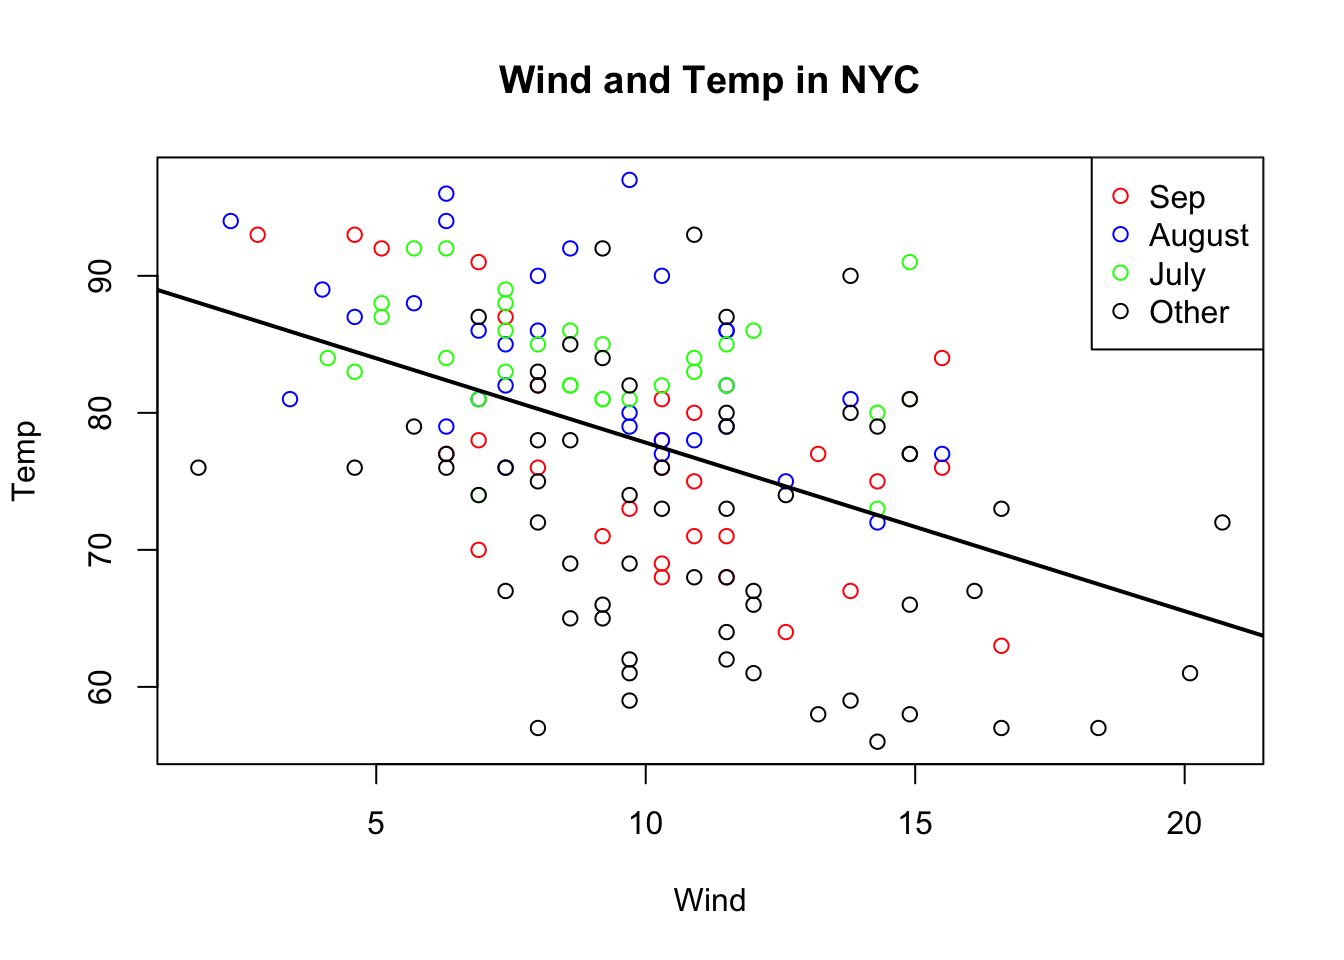
\includegraphics{bookdown-demo_files/figure-latex/unnamed-chunk-87-1.pdf}

\begin{Shaded}
\begin{Highlighting}[]
\CommentTok{#使用基本函数绘图,需要事先计划,运行很多函数,}
\CommentTok{#可以直观的反映我们绘图的逻辑}
\CommentTok{#图例要仔细一一对应}
\end{Highlighting}
\end{Shaded}

lattice 绘图实践

\begin{Shaded}
\begin{Highlighting}[]
\KeywordTok{library}\NormalTok{(lattice) }\CommentTok{#需要先安装install.packages("lattice")}
\KeywordTok{xyplot}\NormalTok{(Temp}\OperatorTok{~}\NormalTok{Ozone, }\DataTypeTok{data=}\NormalTok{airquality) }\CommentTok{#散点图,还没有考察交互关系}
\end{Highlighting}
\end{Shaded}

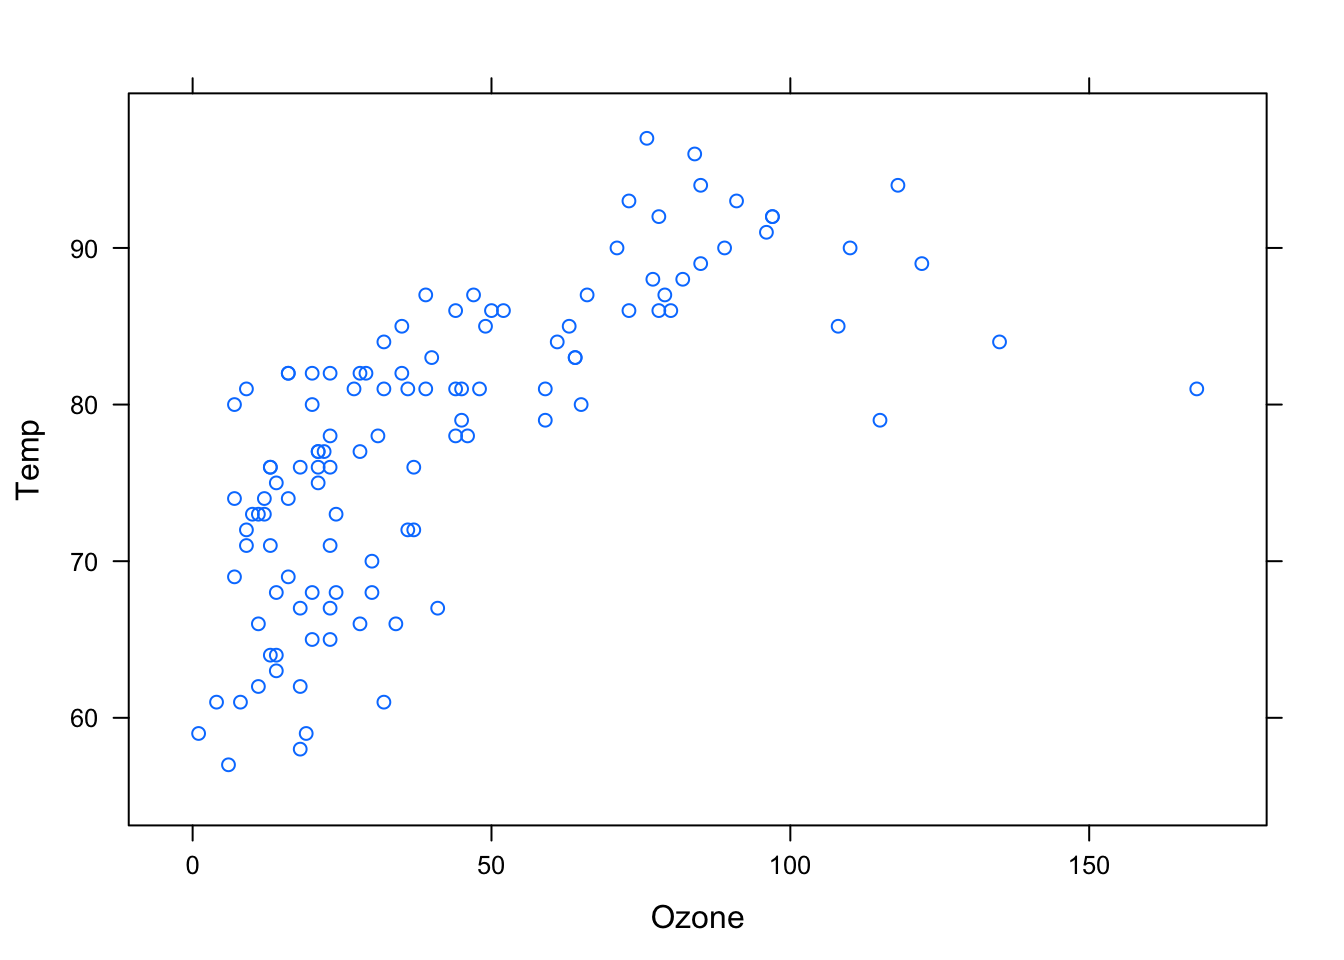
\includegraphics{bookdown-demo_files/figure-latex/unnamed-chunk-88-1.pdf}

\begin{Shaded}
\begin{Highlighting}[]
\NormalTok{airquality}\OperatorTok{$}\NormalTok{Month<-}\KeywordTok{factor}\NormalTok{(airquality}\OperatorTok{$}\NormalTok{Month)}
\end{Highlighting}
\end{Shaded}

使用

\begin{Shaded}
\begin{Highlighting}[]
\CommentTok{#查看不同月份下,前面两个变量的关系}
\KeywordTok{xyplot}\NormalTok{(Temp}\OperatorTok{~}\NormalTok{Ozone}\OperatorTok{|}\NormalTok{Month, }\DataTypeTok{data=}\NormalTok{airquality,}
       \DataTypeTok{layout=}\KeywordTok{c}\NormalTok{(}\DecValTok{5}\NormalTok{,}\DecValTok{1}\NormalTok{)) }\CommentTok{#画1行5列}
\end{Highlighting}
\end{Shaded}

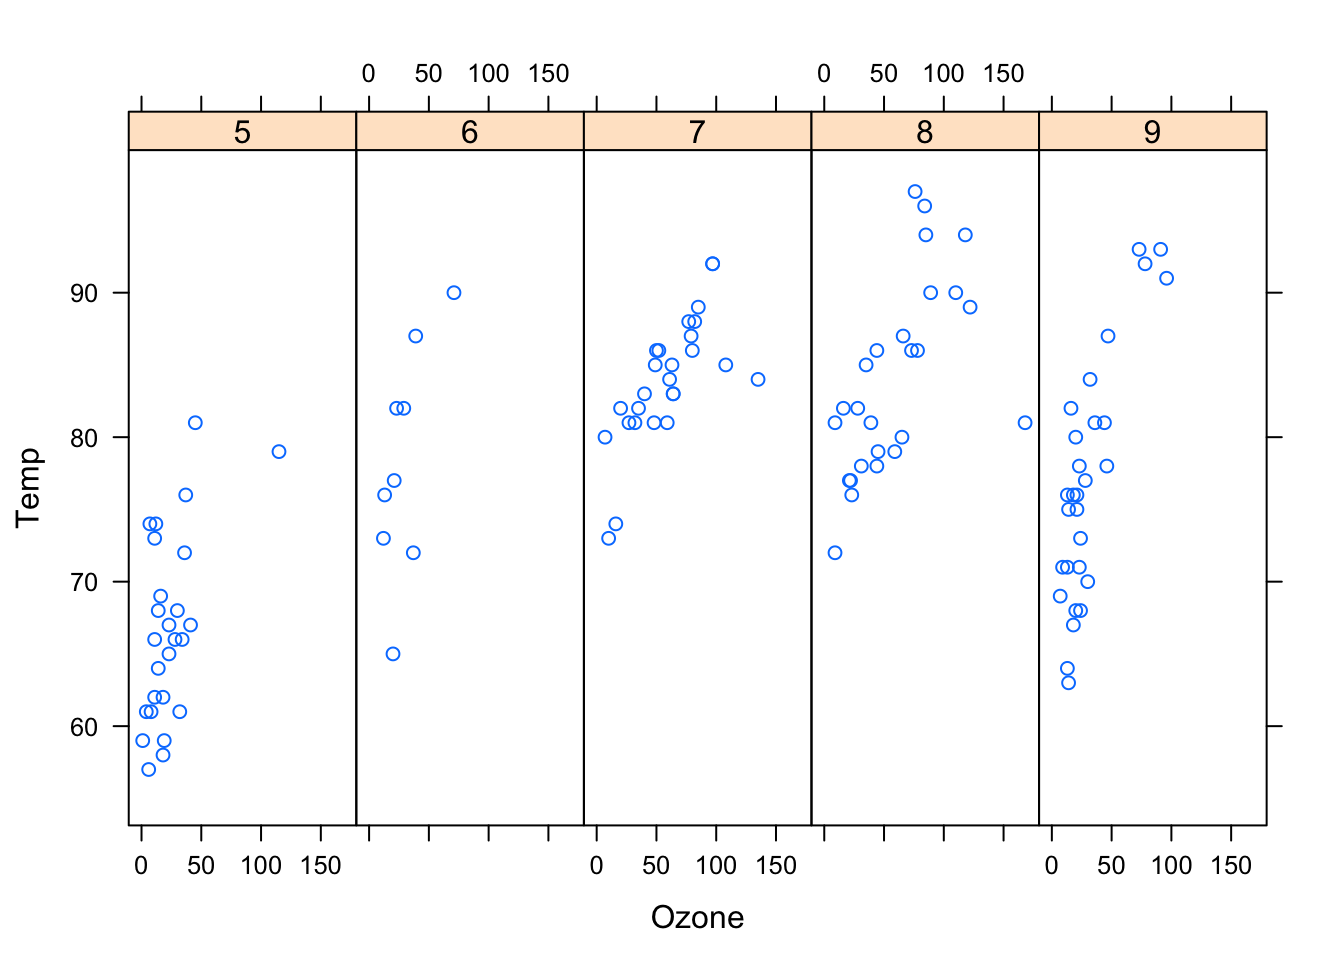
\includegraphics{bookdown-demo_files/figure-latex/unnamed-chunk-89-1.pdf}

绘制表示相关性的椭圆图

越椭圆相关性越高,高到变成一条线。越接近圆相关性越低,直到标准圆。颜色越深相关性越大,最大是1,最小的是0(绝对值),蓝色为正相关,红色为负相关。

\begin{Shaded}
\begin{Highlighting}[]
\CommentTok{# Load the corrplot library for the corrplot() function}
\KeywordTok{library}\NormalTok{(corrplot)}

\CommentTok{# Extract the numerical variables from UScereal}
\NormalTok{numericalVars <-}\StringTok{ }\NormalTok{UScereal[, }\DecValTok{2}\OperatorTok{:}\DecValTok{10}\NormalTok{]}

\CommentTok{# Compute the correlation matrix for these variables}
\NormalTok{corrMat <-}\StringTok{ }\KeywordTok{cor}\NormalTok{(numericalVars)}

\CommentTok{# Generate the correlation ellipse plot}
\KeywordTok{corrplot}\NormalTok{(corrMat, }\DataTypeTok{method =} \StringTok{"ellipse"}\NormalTok{)}
\end{Highlighting}
\end{Shaded}

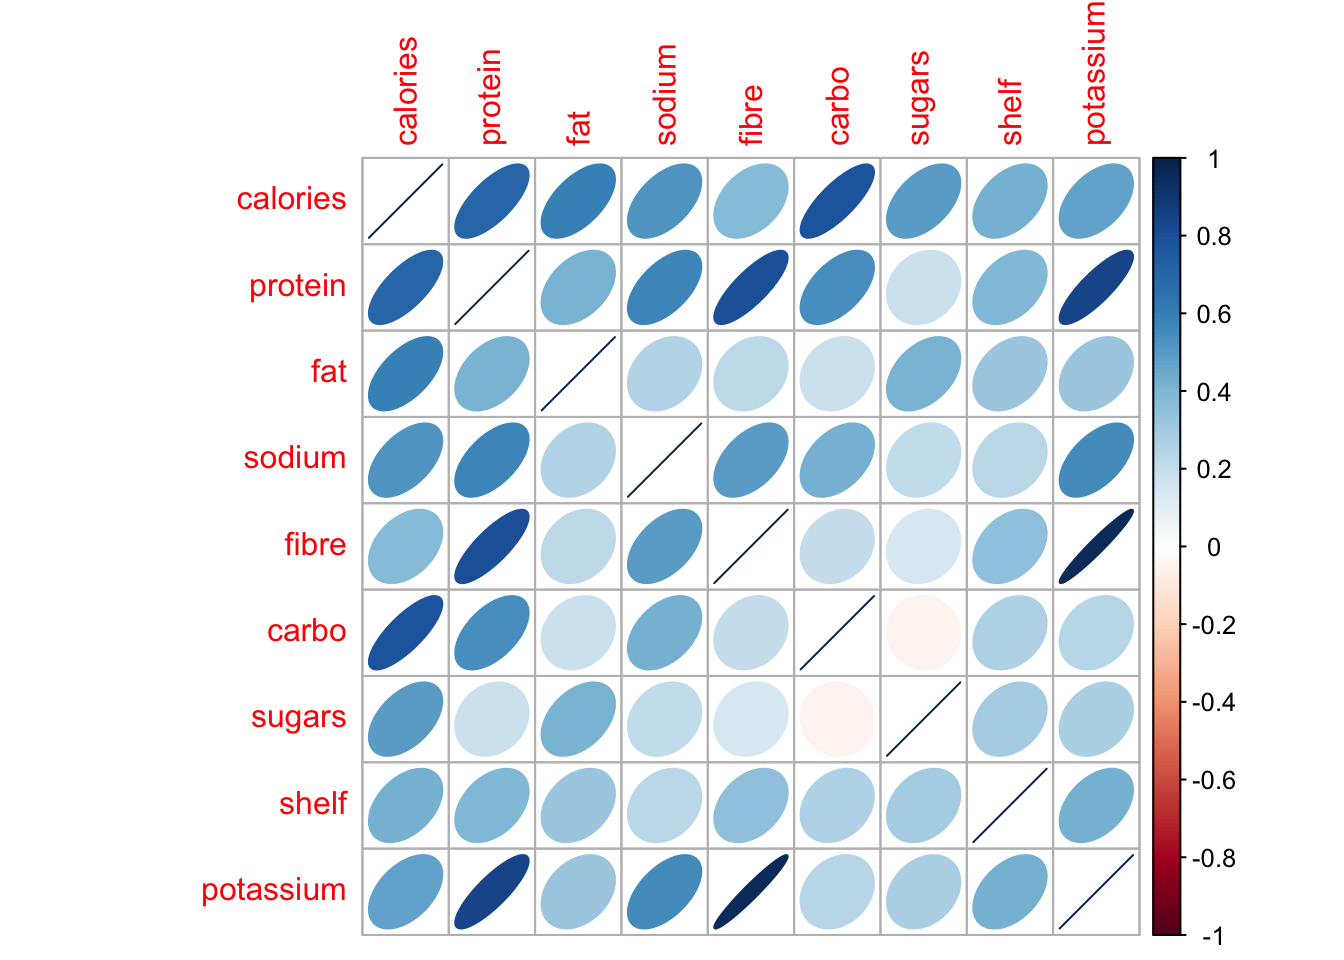
\includegraphics{bookdown-demo_files/figure-latex/unnamed-chunk-90-1.pdf}

主要来自data visulization in
datacamp的第一章第二章(共四章)以及慕课网的数据可视化课程。还可以继续补充。

\chapter{数据可视化第二课:}

\hypertarget{ggplot2-}{%
\section{ggplot2 绘图包介绍}\label{ggplot2-}}

\section{用几何函数指定图形类型}

\section{分组}

\section{刻面}

\section{添加光滑曲线}

\section{保存图}

\chapter{数据可视化第三课:案例}

\section{泰坦尼克号生还者分析}

\chapter{线性回归第一课}

\section{相关性}

\subsection{散点图}

\subsection{相关系数}

\subsection{线性关系}

\section{回归模型}

\subsection{模型理解}

\subsection{模型推导}

\subsection{系数含义}

\chapter{回归分析第二课}

\hypertarget{r}{%
\section{如何用R做线性回归}\label{r}}

\subsection{数据导入}

\subsection{前期清理}

\subsection{基本观察}

\subsection{建立模型}

\section{线性回归结果的理解}

\subsection{系数}

\hypertarget{r-}{%
\subsection{R 方}\label{r-}}

\subsection{显著度}

\subsection{模型评估}

\chapter{回归分析第三课}

案例

\section{大学教授收入分析}

\section{广告投入与销售额分析}

\hypertarget{dplyr}{%
\chapter{dplyr包}\label{dplyr}}

\bibliography{book.bib,packages.bib}


\end{document}
